%-----------------------------------------------------------------------
% This is the main tex file for the thesis that combines the 
% individual chapters & other elements
%
% Author: Daniel Finstad
%
% Revision: $Id$
%
%-----------------------------------------------------------------------

% document class and packages
\documentclass[12pt,notitlepage]{report}
%\usepackage{natbib}
\usepackage{bibunits}
\usepackage{suthesis}
\usepackage{graphicx}
\usepackage{color}
\usepackage{bm}
\usepackage{amsmath}
\usepackage[nolist]{acronym}
\usepackage{multirow}
\usepackage{mathtools}
\usepackage{amssymb}
\usepackage{amsfonts}
\usepackage{rotating}
\usepackage[bookmarksnumbered, bookmarksopen, breaklinks, colorlinks, linkcolor=blue, citecolor=magenta]{hyperref}
\usepackage{subfig}
\usepackage{tabularx}
\usepackage{adjustbox}
\usepackage{booktabs}
\usepackage{changepage}
\usepackage{lscape, rotating}
\usepackage[final]{pdfpages}
\usepackage[dvipsnames]{xcolor}
\usepackage{afterpage}

\pdfoutput=1
\DeclareGraphicsExtensions{.pdf,.png}
\DeclareUnicodeCharacter{2009}{\,} 

\hbadness=10000

% new command definitions
%\newcommand{\half}{\frac{1}{2}}
%\newcommand{\ospsd}{\ensuremath{S_n\left(\left|f_{k}\right|\right)}}
\newcommand{\amber}[1]{{\color{ProcessBlue} [#1]}}
\newcommand{\checkme}[1]{{\color{BrickRed} #1}}
\newcommand{\ecc}{\ensuremath{e}}
\newcommand{\eccthirty}{\ensuremath{e_{30}}}
\newcommand{\chieff}{\ensuremath{\chi_{\mathrm{eff}}}}
\newcommand{\rankingstat}{\ensuremath{\tilde{\rho}_c}}
\newcommand{\tdr}{\ensuremath{\mathrm{TDR}}}
\newcommand{\far}{\ensuremath{\mathcal{F}}}
\newcommand{\tar}{\ensuremath{\mathcal{T}}}
\newcommand{\msun}{\ensuremath{\mathrm{M}_{\odot}}}
\newcommand{\mchirp}{\ensuremath{\mathcal{M}}}
\newcommand{\pastro}{\ensuremath{P_{\mathrm{astro}}}}

% journal definitions
\newcommand{\aj}{{\it Astronomical Journal}}
\newcommand{\apj}{{\it Astrophysical J.}}
\newcommand{\apjl}{{\it Astrophysical J.}}
\newcommand{\aap}{{\it Astron. and Astrophys.}}
\newcommand{\aaps}{{\it Astronomy and Astrophysics, Supplement}}
\newcommand{\aapr}{{\it The Astronomy and Astrophysics Review}}
\newcommand{\actaa}{{\it Acta Astronomica}}
\newcommand{\apjs}{{\it Astrophysical Journal, Supplement}}
\newcommand{\araa}{{\it Annual Review of Astronomy and Astrophysics}}
\newcommand{\aplett}{{\it Astrophysics Letters}}
\newcommand{\cmp}{{\it Commun. Math. Phys.}}
\newcommand{\grg}{{\it Gen. Rel. Grav.}}
\newcommand{\cqg}{{\it Class. Quant. Grav.}}
\newcommand{\lr}{{\it Living Reviews in Relativity}}
\newcommand{\mnras}{{\it Mon. Not. Roy. Astr. Soc.}}
\newcommand{\nar}{{\it New Astronomy Review}}
\newcommand{\pasa}{{\it Publications of the Astron. Soc. of Australia}}
\newcommand{\pasp}{{\it Publ. Astron. Soc. Pac.}}
\newcommand{\pr}{{\it Phys. Rev.}}
\newcommand{\prl}{{\it Phys. Rev. Lett.}}
\newcommand{\prd}{{\it Phys. Rev. D}}
\newcommand{\pra}{{\it Phys. Rev. A}}
\newcommand{\prsl}{{\it Proc. R. Soc. Lond. A}}
\newcommand{\ptrsl}{{\it Phil. Trans. Roy. Soc. London}}
\newcommand{\rmp}{{\it Rev. Mod. Phys.}}

%\newcommand{\tcr}{\textcolor{red}}
%\newcommand{\tcb}{\textcolor{blue}}
%\newcommand{\tcm}{\textcolor{magenta}}
%\newcommand{\tcg}{\textcolor{green}}
%\newcommand{\tcp}{\textcolor{purple}}

\usepackage{color}
\definecolor{cyan}{rgb}{0,0.9,0.9}
\definecolor{orange}{rgb}{0.9,0.5,0}
\definecolor{magenta}{rgb}{1,0,1}
\definecolor{purple}{rgb}{0.5,0.0,0.5}
\definecolor{teal}{rgb}{0.0,0.5,0.5}
\definecolor{gray}{rgb}{0.8242,0.8242,0.8242}
%%
\begin{document}

\Abstract{
Since making the first direct detection of gravitational waves in 2015, the Advanced Laser Interferometer Gravitational-Wave Observatory (LIGO) together with the Virgo observatory has detected an additional 51 confirmed signals from binary mergers. Two of these signals, GW170817 and GW190425, were identified as binary neutron star mergers. As detector sensitivity improves we expect to see many more binary neutron star merger events, both from future observing runs of the LIGO-Virgo network and from planned third-generation detectors. These new detections will provide an exquisite look at the nature of these systems and of neutron stars themselves. This thesis describes how gravitational-wave observations of neutron star mergers can be used to measure the properties of the binary systems and the fundamental physics of neutron stars. We use multimessenger observations of GW170817 to measure its viewing angle, which is important to understand the engine driving the electromagnetic counterpart to the gravitational-wave signal. We describe a new implementation of a fast likelihood model for gravitational-wave parameter estimation. We demonstrate that this likelihood allows analysis of binary neutron star signals to be performed quickly enough to inform strategies for electromagnetic follow-up observations. We measure the tidal deformabilities and radii of the neutron stars in GW170817, imposing a physical constraint to require that both neutron stars obey a common nuclear equation of state. We assess the future prospects for measuring the nuclear equation of state with the LIGO-Virgo network and with the planned third-generation detector, Cosmic Explorer.
}

\title{Binary Neutron Star Mergers: Gravitational-Wave Measurements of their Parameters and the Nuclear Equation of State}
\author{Daniel Finstad}
\majorprof{Duncan A. Brown}
\previousdegree{}{B.A., University of California, 2015}
\submitdate{August 2021}
\degree{Doctor of Philosophy}
\program{Physics}
\copyrightyear{2021}
\majordept{Physics}
%\atitlep
\clearpage

\havededicationtrue
\dedication{To Mom, Dad, \& Lynn}
\haveminorfalse
\copyrightyear{2021}
\copyrighttrue
\doctoratetrue
\figurespagetrue
\tablespagetrue
\electronicsubmittrue
\Acknowledgments{
Acknowledgements stuff goes here}
\beforepreface
\prefacesection{Preface}
Chapter~\ref{ch:inc-angle} is based on material from: \\
\textit{Daniel Finstad}, Soumi De, Duncan A. Brown, Edo Berger, Christopher M. Biwer, ``Measuring the Viewing Angle of GW170817 with Electromagnetic and Gravitational Waves," \textbf{The Astrophysical Journal Letters, Volume 860, Number 1 (2018)} \\
\url{https://iopscience.iop.org/article/10.3847/2041-8213/aac6c1}.
\\ \\
Chapter~\ref{ch:rel-bin-pe} is based on material from:  \\ 
\textit{Daniel Finstad}, Duncan A. Brown, ``Fast Parameter Estimation of Binary Mergers for Multimessenger Followup," \textbf{The Astrophysical Journal Letters, Volume 905, Number 1 (2020)} \\ \url{https://iopscience.iop.org/article/10.3847/2041-8213/abca9e}.
\\ \\
Chapter~\ref{ch:common-radius} is based on material from:  \\ 
Soumi De, \textit{Daniel Finstad}, James M. Lattimer, Duncan A. Brown, Edo Berger, Christopher M. Biwer, ``Tidal Deformabilities and Radii of Neutron Stars from the Observation of GW170817," \textbf{Physical Review Letters, Volume 121, Issue 9 (2018)} \\ \url{https://journals.aps.org/prl/abstract/10.1103/PhysRevLett.121.091102}.
\\ \\


%\\
\afterpreface

\Chapter{Introduction}
\label{ch:intro}
The Advanced LIGO~\cite{TheLIGOScientific:2014jea} and
Virgo~\cite{TheVirgo:2014hva} observatories have completed three observing runs to date, searching for gravitational waves emitted during the inspirals of compact object
binaries, composed of stellar-mass black holes (BHs) or neutron stars (NSs). During the first observing run, the LIGO observatories reported the first direct observations of gravitational waves from a binary black hole merger, GW150914~\cite{Abbott:2016blz}. This observation was followed by two more binary black hole detections in the same observing run~\cite{TheLIGOScientific:2016pea}. During the second observing run, the Virgo observatory joined the LIGO observatories, and reported for the first time, direct detection of gravitational waves from a binary neutron star inspiral~\cite{TheLIGOScientific:2017qsa}. Along with gravitational waves, the same source, referred to as GW170817, was observed across the full electromagnetic spectrum~\cite{GBM:2017lvd}, providing opportunities to answer a whole host of long-standing open questions in physics. In addition to the binary neutron star detection, the second observing run also reported observations of seven binary black hole mergers~\cite{TheLIGOScientific:2014jea,Abbott:2017vtc,Abbott:2017gyy,LIGOScientific:2018mvr,LIGOScientific:2018mvr,LIGOScientific:2018mvr,Abbott:2017oio,LIGOScientific:2018mvr}. From the third observing run, the community has been alerted of 33 merger candidates to date~\url{https://gracedb.ligo.org/superevents/public/O3/}, with one confirmed neutron star merger~\cite{Abbott:2020uma}, one confirmed binary black hole merger~\cite{LIGOScientific:2020stg}, and one black hole - compact object merger, where the compact object could be the highest mass neutron star or the lowest mass black hole discovered for the first time~\cite{Abbott:2020khf}. With the observatories starting to make routine detections, we now have incredible opportunities to probe the properties of neutron stars and black holes, and understand the physics of binary mergers. The plethora of exciting questions relating to compact object mergers can be divided into three broad categories: (i) What are the characteristics of neutron stars and stellar-mass black holes in our universe and how to accurately extract this information from the gravitational waves they emit? (ii) how do these close compact object binaries form? (iii) what are the outcomes of the mergers---what are the astrophysical processes that occur and the remnant objects that form after mergers? In this thesis we study some of the questions under these broad categories. Below we summarize the background of the topics we study and the directions we undertake to pursue these problems.

\section{Information extraction from gravitational-wave signals}
Gravitational waves detected by the LIGO and Virgo observatories carry imprints of properties of the compact objects in their astrophysical source systems. The systems that LIGO-Virgo is searching for comprise black hole - black hole binaries, neutron star - neutron star binaries, and neutron star - black hole binaries. Data streams from the observatories that contain gravitational-wave signals can be analyzed to extract measurable properties of the source binaries---pointing to the characteristics of stellar-mass black holes and neutron stars in our universe. In practice, accurate measurements of signal properties are performed using Bayesian inference~\cite{Bayes:1763,Jaynes:2003jaq}. Bayesian inference allows us to select the signal model that is best supported by observations, and to obtain probability distributions for a model's parameters---serving as measurements of the parameter values. The main source parameters of interest are masses and spins of the component objects, distance to the source, viewing angle of the binary (angle between the binary's angular momentum and line of sight) and sky location of the binary. If the detected source is composed of at least one neutron star, there can be additional parameters, such as tidal deformabilities---we discuss this parameter in detail later in this thesis. 

In Chapter \ref{ch:o2_bbh_pe}, we present Bayesian inference analyses of the seven binary black hole mergers from LIGO-Virgo's second observing run, using the \texttt{PyCBC Inference}~\cite{Biwer:2018osg} software. We describe the methodology used in such analyses to extract information about the parameters of interest from compact object binaries, and present measurements of source properties of the binary black hole mergers.

In Chapter \ref{ch:common_eos}, we use Bayesian parameter estimation to measure parameters of interest from the first observations of gravitational waves from a binary neutron star inspiral, from LIGO-Virgo's second observing run, GW170817. This study was focused on extracting the tidal deformability and radius parameters of the component objects, and the physics questions that the measurements addressed. 

Neutron stars are laboratories for studying matter at the highest densities in the observable universe. The behavior of such incredibly dense matter is described by the nuclear equation of state. Gravitational waves from neutron star mergers can be used to measure the nuclear equation of state. In a neutron star binary system, as the two companions come in close vicinity to each other at the end of their inspiral phase, the gravitational field of each object induces a deformation in the structure of its companion. This deformation is measurable as a parameter, referred to as tidal deformability. The tidal deformability parameter enters into the phase of the gravitational-wave signal emitted from the binary. In addition to the tidal deformability parameter, it is also possible to measure the radius of the component neutron stars using gravitational waves. Both the tidal deformabilities and radii tell us how compact the neutron stars are, and their measurements are critical to determining the nuclear equation of state, as well as for interpreting multimessenger observations of neutron star mergers---observations of the same source with different types of signals or ``messengers''.

We implement a physical constraint on the nuclear equation of state, and information from the electromagnetic observations of GW170817, directly into our Bayesian parameter estimation analysis of the gravitational-wave data, to constrain the tidal deformabilities of the neutron stars of the binary. The constraint we use includes the undeniable correlations relating tidal deformabilities and masses of neutron stars. It is computed using parameterized hadronic equations of state, simulated using a fixed neutron star crust coupled with three polytropic segments. The relation also takes into account causality and the observed minimum value of the neutron star maximum mass. We use the tidal deformability constraints and mass estimates of the binary extracted from the gravitational-wave data to measure the radii of the neutron stars in the detected binary. It is also possible to directly measure the radii from the gravitational-wave data, and this approach is adopted in Ref.~\cite{capano_stringent_2020}.

\section{Formation of compact object binary sources---the common envelope phase}
The compact object binaries observed by LIGO-Virgo are end products of the evolution of binary systems comprised of massive stars. However, the existing problem in this scenario is that these progenitor binary stars are characterized by an orbital separation comparable to an astronomical unit. As gravitational-wave luminosity is inversely proportional to the fifth power of the binary separation~\cite{PhysRev.136.B1224}, widely separated binaries lose energy incredibly slowly and spiral-in negligibly over billions of years. On the other hand, the colliding compact object binary sources observed by LIGO-Virgo imply thet these binaries have initial orbital separations several orders of magnitude smaller than those in the massive star binaries; the stars would need to have an orbital separation comparable to a solar radius, for them to be driven to merger through gravitational-wave emission, within the age of the universe. Therefore, for massive star binaries to produce LIGO-Virgo sources, there needs to be a transformation in the orbit of the parent binary, such that the components are brought in much closer to each together. The standard framework by which this transformation is believed to take place involves the parent binary evolving into a short phase, called ``common envelope'' during its lifetime. This is a critical stage in the binary star system's evolution, when it is tightened by a factor of two or more orders of magnitude through dynamically unstable mass transfer.

The evolution of binary stars through the common envelope phase can be outlined as follows (See \cite{Postnov:2014tza,2013A&ARv..21...59I,Mandel:2018hfr} for details). The parent binary is comprised of a pair of massive stars widely separated by a few astronomical units. The more massive star (primary) leaves the main sequence phase, and expands rapidly. When its radius crosses the Roche lobe radius~\cite{1983ApJ...268..368E}, it starts transferring mass on to the less massive star (secondary), which is still in the main sequence phase. Mass transfer at this step may be non-conservative but is stable. The transfer takes place on the thermal timescale of the primary, with the secondary being unable to assimilate the incoming mass at a thermal equilibrium state, as it is less evolved, and has a longer thermal timescale. At the end of the mass transfer, the primary loses its hydrogen envelope and turns into a helium burning core, which can be identified as a Wolf-Rayet star~\cite{1967AcA....17..355P}, and eventually undergoes a core-collapse supernova explosion, to form a compact object (such as black hole or neutron star). %The secondary star can be spun up by the angular momentum endowed by the transferred matter onto it. 
The secondary eventually grows out of its main sequence phase and the two companions switch roles. The secondary now grows and impinges upon the orbit of the primary (now a compact object). Note that the primary at this point is typically much smaller in size and mass than the secondary, as a result of the processes it has passed through in the course of evolution into a compact object. The mass transfer in this step is non-conservative as well as unstable, resulting in the formation of an shared envelope inside which the two stars evolve. %The compact object gets dragged into the envelope of the more massive star. 
The compact object spirals in towards denser stellar atmospheres, encountering drag forces--that cause a rapid decay in its orbit and results in the tightening of the orbit of the binary. Additionally, the compact object may get modified by accretion of mass onto it from the envelope. At the end of the dynamical inspiral phase, there can be two typical outcomes. The orbital energy deposited into the envelope ejects the envelope, resulting in the formation of a Wolf Rayet star - compact object binary. The Wolf-Rayet star then undergoes a supernova explosion and collapses into a black hole. If the system survives the explosion, a close compact object binary is formed, which emits gravitational radiation, becomes a LIGO-Virgo source, and merges on a timescale less than a Hubble time. Alternatively, if the envelope is retained, the compact object and the core of the companion may merge into a single compact object. One possible outcome in this case, based on the kind of compact object involved in the system, is formation of a Thorne-Zytkow object~\cite{1977ApJ...212..832T,2014MNRAS.443L..94L}.

In Chapter \ref{ch:common_envelope}, we explore the dynamical inspiral phase of common envelope episodes, during which the crucial orbital transformation of the binary takes place. The major challenge in modeling this scenario is that there are huge ranges of spatial and temporal scales involved, that should be simultaneously tackled. Time scales may range between order of seconds to order of a thousand years. Spatial scales may vary between order of a few kilometers to order of a few thousand solar radius~\cite{2013A&ARv..21...59I}. %Time scales may range between the dynamical time scales of a neutron star, for example---order of seconds, to thermal time scales of the envelope---order of a thousand years. This gives $\approx 10^{10}$ order of magnitude difference. Spatial scales may vary between the size of the compact object---order of a few kilometers to size of the envelope---order of a few thousand solar radius~\cite{2013A&ARv..21...59I}. 
Due to these reasons, modeling the full common envelope evolution in a single simulation is a challenging task. Hereby, we approach this problem by breaking down the complex physics of common envelope interactions, and look at individual aspects of the problem with simplified calculations. We isolate the flow around the embedded object from the rest of the envelope, and study its behavior in response to changing surrounding conditions. We repeat these calculations varying the surrounding conditions, to model flow morphologies in various regions along the envelope's radial extent, as well as across the range of typical common envelope encounters. A synthesis of the suite of simulations collectively provides a modeling of the full common envelope dynamical inspiral phase. We use our simulation results to study the evolution of component objects and the orbit of the binary during these episodes. %understand the effect of this phase on the observable properties---such as mass and spin---of the LIGO-Virgo stellar-mass black hole populations.

\section{Outcomes of neutron star mergers}
Unlike black hole mergers, which are purely gravitational events, the merging of a binary that involves a neutron star, such as a neutron star - neutron star or a neutron star - black hole merger, involves matter, which plays a significant role during and after the collision of the two objects. The work of astrophysicists in the past few decades predicted that the energetic processes taking place during the merger and interactions of matter released by the collision with the surrounding medium, give rise to a series a non-thermal and thermal emissions across the electromagnetic spectrum (for example, \cite{Bloom:2008ua,Metzger:2011bv,Piran:2012wd,Rosswog:2015nja,Fernandez:2015use,1986ApJ...308L..43P,Eichler:1989ve,Narayan:1992iy,Nakar:2011,Hotokezaka:2015eja,Li:1998bw,2010MNRAS.406.2650M,2011ApJ...736L..21R}). Furthermore, the work of Ref.~\cite{1974ApJ...192L.145L} predicted that neutron star - black hole mergers would eject significant amounts of neutron rich material into the interstellar medium, which would be promising sources of a phenomenon called rapid neutron capture, or $r$-process nucleosynthesis. Later, Refs.~\cite{1982ApL....22..143S, Eichler:1989ve} suggested that such a process would also take place in case of neutron star - neutron star mergers.  During the $r$-process, heavy seed nuclei in locations of high density neutron rich material undergo a rapid capture of free neutrons, at a high rate, with no time for radioactive decay between captures. These processes are responsible for forming approximately half of the elements in the periodic table that are heavier than iron.

The first observations of a binary neutron star merger by the LIGO-Virgo detectors, GW170817, gave us the opportunity to examine the theoretical predictions of electromagnetic emissions and nucleosynthetic yields associated with the merger. The gravitational-wave signal was followed up exhaustively by a global array of telescopes in search of electromagnetic counterparts~\cite{GBM:2017lvd}. Less than $\sim$ 2 seconds after the merger time extracted from the gravitational-wave signal, a short gamma-ray burst (GRB 170817A) was produced at the same source location. This was followed by an optical transient SS17a/AT2017gfo. The source was eventually observed in X-ray, ultraviolet, infrared, and radio bands over hours, days, and weeks. The optical and infrared transients from this events could be explained to have been triggered by $r$-process events associated with the merger. In the $r$-process nucleosynthesis, after all the free neutrons in the reservoir are consumed by seed nuclei, heavy unstable elements are formed. The unstable elements then emit radioactive energy and decay to form final stable nuclei. Therefore, GW170817 provided evidence of neutron star mergers being the origin of short gamma-ray bursts and kilonovae, and being astrophysical sites for production of heavy elements in the universe.  

There are several ways by which $r$-process material can be ejected in a neutron star merger. One of the mechanisms is via tidal tail ejecta. Close to the time of merger, as two neutron stars or a neutron star and a black hole in the binary come in close vicinity to each other, material can be tidally shredded off each neutron star component by its companion~\cite{Davies:1993zn,Ruffert:1996by,Rosswog:1998hy}. The material typically expands outwards from the merger location in the equatorial plane of the binary. Another mechanism of mass ejection would be via shock heated ejecta. As the two components come into contact with each other, shock heating can give rise to ejecta, that is released out of the polar regions~\cite{Oechslin:2006,PhysRevD.87.024001,Bauswein:2013jpa}. A third type of ejecta can be from postmerger accretion disk outflows. Merger of the binary components leads to the formation of a compact object (black hole or neutron star). Matter released in this process from the neutron star components in the binary, can have sufficient angular momentum to circularize around the remnant compact object in the form of an accretion disk. Eventually, these accretion disks can give rise to strong outflows, that are sites for $r$-process nucleosynthesis~\cite{Metzger:2008av,Dessart:2008zd}. Neutron star mergers involve strong gravitational and magnetic fields, due to which it is appropriate to model them using general-relativistic magnetohydrodynamic simulations. In Chapter \ref{ch:kilonova}, we use such simulations with weak interactions to model postmerger accretion disks, outflows, and nucleosynthetic yields applicable to a variety of neutron star - neutron star and neutron star - black hole merger scenarios. The physics associated with such disks, their $r$-process outcomes, and the kilonova transients they trigger are expected to vary across mergers. These outcomes depend on the initial conditions, which comprise of a complex combination of the masses and spins of the components, the type of components (neutron star - neutron star and neutron star - black hole pairs), as well as the nuclear equation of state. We explore the properties of distinct states of accretion disks and their outcomes across the binary parameter space. We provide theoretical models and predictions that could be tested against a variety of future neutron star merger observations.

\Chapter{Parameter Estimation Techniques}
\label{ch:pe-technique}
\newcommand{\pset}{\vartheta}
\newcommand{\likelihood}{\ensuremath{p(\vec{d}(t)|\vec{\pset},H)}}
\newcommand{\prior}{\ensuremath{p(\vec{\pset}|H)}}
\newcommand{\evidence}{\ensuremath{p(\vec{d}(t)|H)}}
\newcommand{\posterior}{\ensuremath{p(\vec{\pset}|\vec{d}(t),H)}}

We give an overview of the techniques of gravitational-wave parameter estimation, which are employed widely throughout this thesis. We outline the basic principles behind Bayesian inference for gravitational-wave astronomy and the sampling methods we use to produce posterior estimates in our analyses. We also comment on some practical considerations we found useful in the completion of this work, though we emphasize the items we discuss are by no means an exhaustive list.

\section{Bayesian inference}\label{sec:bayesian_inference}
In gravitational-wave astronomy we use Bayesian methods as a convenient way to infer the astrophysical source parameters from a detected signal~\cite{FinnChernoff:1993,Cutler:1994ys,Nicholson:1997qh,Christensen:2001cr}. For a stretch of gravitational-wave detector data $\vec{d}(t)$ identified as containing a gravitational-wave signal, Bayes' theorem~\cite{Bayes:1793,Jaynes:2003} states that for a hypothesis $H$, the posterior probability density is
% joint posterior probability definition
\begin{equation}
\label{eqn:bayes} \posterior =
\frac{\likelihood \prior}{\evidence} .
\end{equation}
Here $p(A|B)$ denotes the conditional probability of $A$ given $B$. In the context of gravitational-wave inference, the hypothesis $H$ is the model of the gravitational waveform, and 
$\vec{\pset}$ is the set of parameters defining this model. Thus the posterior probability density \posterior\ is the conditional probability that the gravitational-wave signal is defined by parameters $\vec{\pset}$, given data $\vec{d}(t)$ and waveform model $H$. The prior probability density \prior\ represents our prior knowledge of the parameters $\vec{\pset}$ before considering the observed data $\vec{d}(t)$. The posterior probability density is proportional to the prior probability density, as the Bayesian framework considers any new observations in the broader context of prior knowledge. The denominator of Eqn.~\ref{eqn:bayes}, \evidence\ is known as the ``evidence" or ``marginal likelihood," and it serves as a normalizing constant to ensure the integral of \posterior\ over the parameter space is equal to unity.

In practice, we are very often interested in posterior estimates of only one or a few parameters. In this case we can obtain marginalized posterior probability density functions by integrating \posterior\ over all unwanted parameters. For instance, given a set of parameters $\vec{\pset}=\left\{ \theta_1,\theta_2,\ldots,\theta_n \right\}$, the marginalized posterior probability density for source parameter $\theta_1$ is
\begin{equation}\label{eqn:margpost}
p(\theta_1|\vec{d}(t),H) = \int \posterior\mathrm{d}\theta_2\mathrm{d}\theta_3\ldots\mathrm{d}\theta_n .
\end{equation}

In a parameter estimation analysis of gravitational-wave data, an implicit assumption is made that the gravitational-wave detector noise is stationary, Gaussian, and uncorrelated between detectors in the network. The data stream from the $i$-th detector in a network is then $d_{i}(t)=n_{i}(t)+s_{i}(t)$, where $s_{i}(t)$ is the gravitational waveform and $n_{i}(t)$ is the Gaussian detector noise. Under these assumptions, the likelihood in Eqn.~\ref{eqn:bayes} has the form~\cite{wainstein:1962}
% likelihood
\begin{eqnarray}\label{eqn:log_likelihood}
\likelihood = \exp \left[ -\frac{1}{2} \sum_{i = 1}^{N} \left<\tilde{n}_{i}(f) | \tilde{n}_{i}(f)\right> \right] \nonumber\\ 
= \exp \left[ -\frac{1}{2} \sum_{i = 1}^{N} \left<\tilde{d}_{i}(f) - \tilde{s}_{i}(f, \vec{\pset})| \tilde{d}_{i}(f) - \tilde{s}_{i}(f, \vec{\pset})\right> \right] ,
\end{eqnarray}
where $N$ is the number of detectors in the network.
The inner product $\langle\tilde{a} | \tilde{b}\rangle$ is
\begin{equation}
\left<\tilde{a}_i(f) | \tilde{b}_i(f)\right> = 4\Re \int_{0}^{\infty} \frac{\tilde{a}_i(f) \tilde{b}_i(f)}{S^{(i)}_n(f)} \mathrm{d}f \,,
\end{equation}
where $S^{(i)}_n(f)$ is the power spectral density of the $i$-th
detector's noise.  Here, $\tilde{d}_{i}(f)$ and $\tilde{n}_{i}(f)$ are the
frequency-domain representations of the data and noise, obtained by a Fourier
transformation of $d_{i}(t)$ and $n_{i}(t)$, respectively.  The model waveform
$\tilde{s}_{i}(f, \vec{\pset})$ may be computed directly in the frequency
domain, or in the time domain and then Fourier transformed to the frequency
domain.

\section{Sampling}
In order to explore the parameter space and produce marginalized posterior distributions for astrophysical parameters of interest we use a variety of stochastic sampling techniques. For all sampling methods though the general principle is the same.

\subsection{Markov Chain Monte Carlo}
% basic markov chain and ensemble sampling
A common sampling technique is Markov Chain Monte Carlo (MCMC) where the sampler will assemble a chain of samples drawn from the parameter space according to several rules. The first sample in the chain is drawn randomly from the prior probability density function, then at each iteration a new sample is proposed. Each proposed sample is accepted or rejected according to a tunable acceptance probability, which depends on a comparison of the likelihoods of the previous and proposed samples. If the proposed sample is accepted it is appended to the chain, otherwise the previous sample is repeated instead. The cycle then repeats and sampling proceeds until the desired stopping criteria are satisfied. Ensemble MCMC sampling, where multiple Markov chains are initialized and advanced independently, is also commonly used as a more efficient means to explore a large parameter space.

% autocorrelation length and independent samples
Neighboring samples in a Markov chain are not independent of one another, since the nature of the sampling technique has each sample in the chain rely on the previous sample~\cite{Christensen:2004jm}. In order to identify samples in the chain that are independent, we calculate the autocorrelation length $\tau_K$, which is the characteristic length over which samples can be considered independent~\cite{Madras:1988ei}. For a Markov chain $X_l$ of length $l$, the autocorrelation length is
\begin{equation}\label{eqn:acl}
\tau_K = 1 + 2\sum_{i=1}^{K}\hat{R}_{i} ,
\end{equation}
where $K$ is the index of the first sample in the Markov chain satisfying $5\tau_K \leq K$. The autocorrelation function $\hat{R}_{i}$ is defined as
\begin{equation}\label{eqn:acf}
\hat{R}_{i} = \frac{1}{l \sigma^{2}} \sum_{t=1}^{l-i} \left( X_{t} - \mu \right) \left( X_{t+i} - \mu \right),
\end{equation}
where $X_t$ are the samples of $X_{l}$ between the 0-th and the $t$-th sample, $X_{t+i}$ are the samples of $X_{l}$ between the 0-th and the $(t+1)$-th sample, and $\mu$ and $\sigma^2$ are the mean and variance of $X_t$ respectively. We can then extract samples from a Markov chain that are representative of the posterior probability density function by drawing samples from the chain spaced by an interval of the autocorrelation length~\cite{Christensen:2004jm}.

% parallel-tempered sampling
An additional modification to typical MCMC sampling is to create parallel copies of each Markov chain at different ``temperatures," and advance chains of each temperature independently. Chains at a temperature $T$ will explore a modified likelihood so that the posterior probability density function becomes
\begin{equation}
p_{T}(\vec{\pset}|\vec{d}(t),H) = \frac{ \likelihood^{\frac{1}{T}} \prior }{p(\vec{d}(t)|H)} .
\end{equation}
This modification causes the Markov chains with a higher temperature to explore an effectively flatter likelihood landscape, increasing the probability that proposed steps are accepted and thus making these chains more likely to fully explore the parameter space and potentially find largely separated modes of high likelihood. As $T \to \infty$, the posterior probability density becomes just the (normalized) prior probability density. At each iteration the position of Markov chains are swapped between temperatures using an acceptance criteria described in Ref.~\cite{vousden:2016}, allowing information of the likelihood across the entire parameter space to propagate among all the chains. Upon completion of the analysis, posterior samples are taken only from chains where $T=1$, with independent samples extracted from the chains as described above.

\subsection{Nested sampling}
An alternative to MCMC sampling is ``nested" sampling~\cite{Skilling:2006,Feroz:2007kg,Speagle_2020}, which was initially designed as a means of efficiently computing the evidence but will also produce marginal posteriors as a useful byproduct.
Nested sampling does not rely on chains of samples, but rather a constantly updating set of ``live points." To initialize the sampling, $N_{\mathrm{live}}$ samples are drawn from the prior volume and the likelihood $\mathcal{L}$ for each is calculated. Then at each iteration $i$ the live point with the lowest likelihood $\mathcal{L}_i$ is dropped from the set, and a new sample is drawn with the condition $\mathcal{L} > \mathcal{L}_i$. In this way, a nested sampler will progress through nested ``shells" of increasing likelihood, contracting onto any regions of high likelihood in the parameter space. The remaining prior volume $X_i$, defined as the fraction of the prior volume contained within an iso-likelihood contour with $\mathcal{L}=\mathcal{L}_i$, is then a monotonically decreasing sequence with
\begin{equation}
    1=X_0>X_1>\cdots>X_M>0
\end{equation}
after $M$ iterations. The evidence $\mathcal{Z}$ can then be numerically approximated by calculating the weighted sum over the discarded samples
\begin{equation}\label{eqn:quadsumev}
    \mathcal{Z} = \sum_{i=1}^{M} \mathcal{L}_{i}w_{i} ,
\end{equation}
where the weights $w_i$ are determined by the quadrature method used, and adding the contribution from the set of live points
\begin{equation}
    \mathcal{Z}_{\mathrm{live}} = \frac{X_M}{N_{\mathrm{live}}} \sum_{j=1}^{N_{\mathrm{live}}} \mathcal{L}_j .
\end{equation}
Upon completion of the run, every sample in the collection of discarded and live points is assigned the posterior weight~\cite{Feroz:2008xx}
\begin{equation}\label{eqn:nestpostweight}
    p_{j} = \frac{\mathcal{L}_{j}w_{j}}{\mathcal{Z}} ,
\end{equation}
where $j$ goes from $1$ to $M+N_{\mathrm{live}}$, and $w_{j>M}=X_M/N_{\mathrm{live}}$.
These posterior weights can then be used to draw posterior samples from the full sequence of sampled points in the analysis~\cite{Feroz:2008xx}.

Nested sampling is preferable to an MCMC sampler when calculating evidence, as the nested sampling algorithm more efficiently explores the full parameter space. However, the nested samplers available in \textit{PyCBC Inference} are more restrictive in the prior distributions that can be used; they draw samples from a unit interval for each source parameter in the analysis and require a transformation from this space to the desired prior probability distribution. We have also observed nested samplers will sometimes fail to produce reasonable posterior estimates for loud signals, which we discuss in more detail in the next section. In the case where the necessary prior transformation is unavailable, or when analyzing loud signals, an MCMC sampler will perform better than the nested samplers.


\section{Practical considerations}
In this section we describe specific details on the implementation of the principles of Bayesian parameter estimation for gravitational-wave astronomy. In particular, we outline the parameterized waveform models describing the binary inspiral signals that we seek to measure, and additional considerations about specific likelihood models and samplers that are used in this thesis.

\subsection{Waveform model}
The intrinsic parameters describing the gravitational wave radiated by a binary merger in its source frame include the component masses $m_{1,2}$, the three-dimensional spin vectors $\vec{s}_{1,2}$ of the compact objects~\cite{Hawking:1987en}, and the eccentricity $e$ of the binary~\cite{Peters:1964zz}. The ``coalescence phase'' $\phi$ describes the phase of the binary at a fiducial reference time, which is often taken to be the phase at the time of merger. For binaries containing neutron stars, additional parameters $\Lambda_{1,2}$ describe the tidal deformabilities~\cite{Flanagan:2007ix,Hinderer:2007mb} of the stars which depend on the equation of state and the masses. The signal observed by a gravitational-wave detector network on Earth depends on six additional parameters: the geocentric time of arrival $t_c$, the luminosity distance to the binary $d_L$, and four Euler angles that describe the transformation of the binary's source frame to the local frame of the detector network. These four angles are defined by the binary's right ascension $\alpha$, declination $\delta$, polarization angle $\Psi$, and inclination angle $\iota$ (the angle between the line of sight and the angular momentum axis of the binary).

The binary's gravitational-wave phasing depends at leading order
on its chirp mass $\mathcal{M} = (m_1 m_2)^{3/5} (m_1 + m_2)^{-1/5}$, where
$m_{1}$ and $m_{2}$ are the binary's component masses~\cite{Peters:1963ux}; 
this quantity will be most accurately measured 
in a gravitational-wave detection. The mass ratio $\eta = m_1 m_2 / (m_1 +
m_2)^2$ enters through higher-order corrections and is less accurately
measured. 
In this thesis, we restrict to binaries where the angular momenta $\chi_{1,2} = J_{1,2} /
m_{1,2}^2$ of each compact object (often refereed to as the compact object's spins) are aligned with the orbital angular momentum vector of the binary, reducing the number of spin parameters in the waveform from six to two. We also only consider binaries in quasi-circular orbits, so $e=0$.

The static neutron star tidal effects first enter at fifth post-Newtonian order
and depend on the tidal deformability of each star $\Lambda_i$~\cite{Flanagan:2007ix,Hinderer:2009ca}.
The parameter $\Lambda_i$ measures how much each neutron star deforms in the presence
of a tidal field, and depends on the neutron star mass and equation of state implicitly through its
dimensionless Love number $k_{2,i}$ and radius $R_i$:
$\lambda_i=(2/3)k_{2,i}R_i^5$. At leading order, the tidal effects are imprinted in
the gravitational-wave signal through the effective tidal deformability parameter
\begin{equation}
\tilde{\Lambda}
= \frac{16}{13}\frac{(12q+1)\Lambda_1+(12+q)q^4\Lambda_2}{(1+q)^5}, \label{eq:pe_tech_lambda_t0}
\end{equation}
where $q = m_2/m_1 \leq 1$ is the binary's mass ratio. We ignore the dynamic tides in this thesis, as they do not significantly affect the waveform for the systems considered.


Given a full set of parameters $\vec{\pset}$ one can generate a model of a gravitational-waveform from a binary merger using a variety of methods. These methods include: full numerical solutions of the Einstein equations (see Ref.~\cite{Cardoso:2014uka} and references therein), perturbation theory~\cite{Teukolsky:1972my,Berti:2009kk}, analytic models calibrated against numerical simulations~\cite{Buonanno:1998gg,Buonanno:2000ef,Damour:2000we,Damour:2001tu,Ajith:2007qp,Ajith:2009bn,Santamaria:2010yb}, and post-Newtonian (pN) theory (see e.g. Ref.~\cite{Blanchet2006} and references therein). 

Gravitational-wave signals  consist of a superposition of harmonic
modes. However, sub-dominant harmonics are too weak to be measured, and so in many cases it is sufficient to model only the dominant mode. In this case, the gravitational-wave signal has the same simple dependence on the fiducial phase $\phi$ in all detectors,
\begin{equation}
\tilde{s}_i(f, \vec{\pset}, \phi) = \tilde{s}_i^0(f, \vec{\pset}, 0) e^{i\phi}.
\end{equation}
The posterior probability $\posterior$ can be analytically marginalized over $\phi$
for models that use this simplification~\cite{wainstein:1962}. If we assume a uniform prior on
$\phi \in [0,2\pi)$, then using the notation of Section~\ref{sec:bayesian_inference} the logarithm of the marginalized posterior is
\begin{eqnarray}
\label{eqn:marginalized_phase}
\log \posterior &\propto \log \prior +
        I_0\left(\left|\sum_i O(\tilde{s}^0_i, \tilde{d}_i)\right|\right) \nonumber \\
        & \qquad - \frac{1}{2}\sum_i\left[ \left<\tilde{s}^0_i, \tilde{s}^0_i\right> -
                                \left<\tilde{d}_i, \tilde{d}_i\right> \right],
\end{eqnarray}
where
\begin{equation*}
\tilde{s}_i^0 \equiv \tilde{s}_i(f, \vec{\pset}, \phi=0),
\end{equation*}
\begin{equation*}
O(\tilde{s}^0_i, \tilde{d}_i) \equiv 4 \int_0^\infty
        \frac{\tilde{s}_i^*(f; \pset,0)\tilde{d}_i(f)}{S^{(i)}_n(f)}\mathrm{d}f,
\end{equation*}
and $I_0$ is the modified Bessel function of the first kind.

In this thesis we use the TaylorF2~\cite{Sathyaprakash:1991mt,Buonanno:2009zt,Arun:2008kb,Mikoczi:2005dn,Bohe:2013cla,Vines:2011ud}, IMRPhenomD~\cite{Husa:2015iqa,Khan:2015jqa}, and IMRPhenomD\_NRTidal~\cite{Husa:2015iqa,Khan:2015jqa,Dietrich:2017aum} waveform models. TaylorF2 is a post-Newtonian waveform model, accurate to 3.5 pN order in orbital phase, 2.0 pN order in spin--spin, quadrupole--monopole and self-spin interactions, and 3.5 pN order in spin--orbit interactions. IMRPhenomD is a phenomenological model tuned to numerical relativity data, and includes representations of each of the inspiral, merger, and ringdown portions of a signal. IMRPhenomD\_NRTidal builds on the IMRPhenomD model by adding corrections to the gravitational-wave phase due to the tidal deformabilities of neutron stars. All waveforms are generated using their respective LIGO Algorithm Library~\cite{lal} implementation.

\subsection{emcee\_pt}
Several of the analyses in this thesis use the parallel-tempered MCMC sampler \\ \texttt{emcee\_pt}~\cite{Foreman_Mackey_2013,Vousden_2015}. In these analyses we found frequently that the sampler would fail to converge in a reasonable time, with the number of independent samples staying constant at around 3000 which results in a poorly sampled posterior distribution. \textit{PyCBC Inference} allows for specifying initial distributions for the MCMC chains, as opposed to having their positions drawn randomly from the prior. We found that drawing the initial positions from Gaussian distributions for each parameter, centered near the peak of the likelihood, would result in full convergence in a reasonably short amount of time. In practice, the location of the likelihood peak can be determined by a trial run where the chains are initialized from the full prior distribution, or is known \textit{a priori} as is the case when analyzing a simulated signal.

Another consideration for the \texttt{emcee\_pt} sampler is the number of temperatures to be used in the analysis. In \textit{PyCBC Inference} this is a tunable setting which can be specified by supplying either an integer, in which case the sampler will automatically pick the temperature spacing, or as an array of inverse-temperatures, with each inverse-temperature specified by $\beta_i=1/T_i$. Generally, a sufficient number of temperatures, and appropriate placement of them, is an important consideration when performing analyses meant to calculate evidence, as this calculation is done via thermodynamic integration and can easily produce inaccurate results for poor choices of temperatures. However in the analyses we perform we are only concerned with measuring posterior probability distributions for various parameters of interest, and as such we found that using $3$ temperatures with the sampler's automatic spacing was sufficient.

\subsection{dynesty}
In Ch.~\ref{ch:rel-bin-pe} we use the \texttt{dynesty} nested sampler~\cite{Speagle_2020} for our analysis. We found that when sampling in component masses $m_{1,2}$, this sampler would sometimes struggle to explore the parameter space fully. As a result the sampler would miss regions of high likelihood, and would prematurely claim to have reached its stopping criteria. The posterior distributions in these cases would appear ``patchy," with many small, disjoint regions. We found that in many cases this problem could be avoided by sampling in the natural mass coordinates of a gravitational-wave signal according to post-Newtonian theory, namely the chirp mass $\mathcal{M}$ and mass ratio $q=m_1/m_2$ or symmetric mass ratio $\eta=m_{1}m_{2}/(m_{1}+m_{2})^2$. However for very loud signals, with signal-to-noise ratio $\rho \gtrsim 75$, we sometimes saw the same issue even when sampling in the natural mass coordinates. We did not find any satisfactory solution to this problem in the case of loud signals, so for these signals we recommend the use of a different sampler.

\subsection{Long duration signals}
Gravitational-wave detectors that use an L-shaped interferometer design, such as the two LIGO detectors and the Virgo detector, have the greatest sensitivity in the direction normal to the plane of the detector arms. This direction is a time-dependent quantity though, as the Earth rotates and moves along its orbit around the sun. Typical parameter estimation analyses will neglect any time-dependence in the detector sensitivity, as the duration of a signal in the sensitive frequency band of current generation detectors is only a few minutes, over which time the antenna pattern can be reasonably approximated as constant. However, third-generation detectors such as Cosmic Explorer will have good sensitivity down to much lower frequencies, which can translate into a low-mass binary inspiral signal staying in the sensitive band for an hour or longer. At this point the time-dependence of the detector antenna pattern becomes non-negligible and it is important that the template waveform used in a likelihood calculation accounts for the variation in sensitivity over its duration. Currently, the relative likelihood model in \textit{PyCBC Inference} has an option which will apply a time-dependent detector antenna response to the template waveforms, and we use this functionality for analyses in this work that use a third-generation detector.

\subsection{Relative likelihood}
In Ch.~\ref{ch:rel-bin-pe} and Ch.~\ref{ch:eos-meas} we use the relative likelihood model available in \textit{PyCBC Inference} which uses an approximation to the likelihood near its peak in order to reduce run time~\cite{Cornish:2010kf,Zackay:2018qdy,Finstad:2020sok}. In practice, the use of this likelihood model requires some care as the approximation it uses is not valid far from the peak of the likelihood. A specific failure mode we encountered would happen when attempting to explore a large prior volume, which allowed sampling parameter space far from the likelihood peak. In this failure mode we would see the analysis would ``run away" to erroneously large likelihoods, generally for parameter values near the boundaries of the prior volume. To prevent this failure we found that placing a mild restriction on the prior volume was broadly effective. Specifically we found that restricting the chirp mass $\mathcal{M}$ to within $\sim 20\%$ of the expected signal would ensure proper convergence. Alternatively (or in addition) the relative likelihood model can be tuned to use more frequency bins in the likelihood calculation which we found would sometimes also prevent this failure.

\Chapter{Measuring the Viewing Angle of GW170817 with Electromagnetic and Gravitational Waves}
\label{ch:inc-angle}
The joint detection of gravitational waves (GWs) and electromagnetic (EM) radiation from the binary neutron star merger GW170817 ushered in a new era of multi-messenger astronomy. Joint GW--EM observations can be used to measure the parameters of the binary with better precision than either observation alone. Here, we use joint GW--EM observations to measure the viewing angle of GW170817, the angle between the binary's angular momentum and the line of sight. We combine a direct measurement of the distance to the host galaxy of GW170817 (NGC\,4993) of $40.7\pm 2.36$ Mpc with the Laser Interferometer Gravitational-wave Observatory (LIGO)/Virgo GW data and find that the viewing angle is $32^{+10}_{-13}\,\pm 1.7$ degrees (90\% confidence, statistical, and systematic errors). We place a conservative lower limit on the viewing angle of $\ge 13^\circ$, which is robust to the choice of prior. This measurement provides a constraint on models of the prompt $\gamma$-ray and radio/X-ray afterglow emission associated with the merger; for example, it is consistent with the off-axis viewing angle inferred for a structured jet model. We provide for the first time the full posterior samples from Bayesian parameter estimation of LIGO/Virgo data to enable further analysis by the community.

\section{Introduction}
On 2017 August 17, the Advanced Laser Interferometer Gravitational-wave Observatory (LIGO) and Virgo observed the gravitational waves (GWs) from a binary neutron star merger, dubbed GW170817 \cite{TheLIGOScientific:2017qsa}. This signal was followed $1.7$ s later by a short gamma-ray burst (GRB), GRB170817A, detected by the {\it Fermi} and {\it INTEGRAL} satellites \cite{Goldstein:2017mmi,Savchenko:2017ffs}. Rapid follow-up of the LIGO/Virgo sky localization region led to the identification of an optical counterpart in the galaxy NGC\,4993 \cite{Coulter:2017wya,Soares-Santos:2017lru,Valenti:2017ngx}, which in turn enabled multi-wavelength observations spanning from radio to X-rays. 

Ultraviolet, optical, and near-infrared observations covering the first month post-merger led to the inference of a complex ejecta structure in terms of mass, velocity, and opacity (e.g., \cite{Chornock:2017sdf,Cowperthwaite:2017dyu,Kasliwal:2017ngb,Nicholl:2017ahq,Pian:2017gtc,Smartt:2017fuw,Villar:2017wcc}), potentially indicative of non-spherical angular structure.  Radio and X-ray observations revealed brightening emission for the first $\approx 5$ months, which has been interpreted as resulting from an off-axis structured relativistic jet (e.g., \cite{Alexander:2017aly,Alexander2018,Lazzati:2017zsj,Margutti:2017cjl,Margutti:2018xqd}), or alternatively a spherical ``cocoon'' of mildly relativistic ejecta (e.g., \cite{Mooley:2017enz}).

Measuring the angle between the binary's angular momentum axis and the line of sight is important for an understanding of the engine powering the multi-wavelength electromagnetic (EM) emission from GW170817.  Following \cite{TheLIGOScientific:2017qsa}, we define the viewing angle  $\Theta=\min(\theta_{JN},180^\circ - \theta_{JN})$, where $\theta_{JN}$ is the angle between the binary's total angular momentum and the line of sight \cite{TheLIGOScientific:2017qsa}. For systems where the angular momentum of each compact object (the spin) is small, and precession of the binary's orbital plane is not significant (as is the case for GW170817), $\theta_{JN} \approx \iota$, where $\iota$ is the angle between the binary's orbital angular momentum and the line of sight (the inclination angle). There is a degeneracy between the binary's inclination, $\iota$, and the luminosity distance, $d_L$, when only LIGO/Virgo observations are used to measure the inclination angle \cite{Wahlquist:1987rx}. Breaking this degeneracy with an independent distance measurement immediately allows one to place tighter constraints on the inclination angle \cite{Fan:2014kka}.

Using GW observations alone, LIGO and Virgo constrained the viewing angle to $\Theta \le 55^\circ$ at 90\% confidence with a low-spin prior \cite{TheLIGOScientific:2017qsa}. To provide an independent distance measurement, Abbott {\it et al.} used the estimated Hubble flow velocity for NGC\,4993 of $3017\pm 166$ km s$^{-1}$ and a flat cosmology with $H_0=67.90\pm 0.55$ km s$^{-1}$ Mpc$^{-1}$ to constrain $\Theta\le 28^\circ$\cite{TheLIGOScientific:2017qsa}. \cite{Mandel:2017fwk} used the combined $H_0$-inclination posterior from \cite{Abbott:2017xzu} in conjunction with the Dark Energy Survey measurement of $H_0=67.2^{+1.2}_{-1.0}$ km s$^{-1}$ Mpc$^{-1}$ \cite{Abbott:2017smn} to infer $\Theta\le 28^\circ$ at 90\% confidence \cite{Mandel:2017fwk}. These circuitous approaches to breaking the distance-inclination degeneracy were motivated partly by the absence of a precise distance measurement to NGC\,4993, as well as by the lack of a published distance-inclination posterior probability distribution. Furthermore, \cite{Mandel:2017fwk} was not able to place a strong constraint on the lower bound of $\Theta$, as his analysis used the GW posteriors \cite{Mandel:2017fwk} and was constrained by LIGO/Virgo's choice of prior in their GW analysis \cite{Abbott:2017xzu}. 

Here, we directly use the most precise distance measurement available for NGC\,4993 of $d_L=40.7\pm 2.36$ Mpc \cite{Cantiello:2018ffy} and the LIGO/Virgo GW data \cite{TheLIGOScientific:2017qsa} to infer $\Theta$ directly from joint GW--EM observations using Bayesian parameter estimation \cite{emcee,pycbc-inference,pycbc-software}. To allow our results to be used by the community for further analysis we provide the full posterior samples from our analysis as supplemental materials.

\section{Methods} \label{sec:methods}

We use Bayesian inference to measure the parameters of GW170817 \cite{Christensen:2001cr}. We calculate the posterior probability density function, $p(\bm{\theta}|\bm{d}(t),H)$, for the set of parameters $\bm{\theta}$ for the GW model, $H$, given the LIGO Hanford, Livingston, and Virgo GW data $\bm{d}(t)$:
\begin{equation}
p(\bm{\theta}|\bm{d}(t),H) = \frac{p(\bm{\theta}|H) p(\bm{d}(t)|\bm{\theta},H)}{p(\bm{d}(t)|H)}, 
\label{eq:rel_bin_postpdf}
\end{equation}
where $\bm{\theta}$ is the vector of the gravitational waveform parameters. The prior, $p(\bm{\theta}|H)$, is the set of assumed prior probability distributions for the waveform parameters. The likelihood $p(\bm{d}(t)|\bm{\theta},H)$ assumes a Gaussian model of detector noise and depends upon the noise-weighted inner product between the gravitational waveform and the GW detector data $\bm{d}(t)$~\cite{Finn:2000hj,Rover:2006bb}. Marginalization of the likelihood to obtain the posterior probabilities is performed using Markov Chain Monte Carlo (MCMC) techniques. Our implementation used the \textit{PyCBC Inference} software package \cite{pycbc-inference,pycbc-software} and the parallel-tempered \textit{emcee} sampler \cite{emcee}. 

The MCMC is performed over the detector-frame chirp mass of the binary $\mathcal{M}^\mathrm{det}$, the mass ratio $q = m_1/m_2, m_1 \ge m_2$, the component spins $\chi_{1,2}$, the time of coalescence $t_c$, the phase of coalescence $\phi_c$, the GW polarization angle $\psi$, the inclination angle of the binary $\iota$, R.A. and decl. of the binary, and the luminosity distance $d_L$. 

We assume a uniform prior distribution on the binary component masses, $m_{1,2}\in [1.0, 2.0]~M_{\odot}$, transformed to $\mathcal{M}^\mathrm{det}$ and $q$ with a cut on the detector-frame chirp mass $1.1876 \le \mathcal{M}^\mathrm{det} \le 1.2076$. We assume a uniform prior on the dimensionless angular momentum of each neutron star, $\chi_{1,2}\in [-0.05, 0.05]$ \cite{Brown:2012qf}. The prior on $t_c$ is uniform in the GPS time interval $[1187008882.3434,1187008882.5434]$. We assume a uniform prior between $0$ and $2\pi$ for $\phi_c$ and $\psi$. We incorporate EM information through fixing the R.A. and decl. of GW170817 and through the prior probability distribution on the luminosity distance $p(d_L|H)$. We run the MCMC with two prior distributions on the inclination angle $\iota$: a prior uniform in $\cos \iota$, and a prior uniform in $\iota$ to explore the posterior distribution for small viewing angles.

We use GW strain data from the Advanced LIGO and Virgo detectors for the GW170817 event, made available through the LIGO Open Science Center (LOSC) \cite{Vallisneri:2014vxa}. The \texttt{LOSC\_CLN\_16\_V1} data that we use here include a post-processing noise subtraction performed by the LIGO/Virgo Collaboration \cite{gw170817-losc,gw170817-noise}. The LOSC documentation states that these data have been truncated to remove tapering effects due to the cleaning process, however the LOSC data shows evidence of tapering after GPS time $1187008900$ in the LIGO Hanford detector. To avoid any contamination of our results we do not use any data after GPS time $1187008891$.  

We high-pass the GW data using an eighth-order Butterworth filter that has an attenuation of $0.1$ at 15~Hz. The filter is applied forward and backward to preserve the phase of the data. A low-pass (anti-aliasing) finite impulse response filter is applied prior to resampling the data. The data is decimated to a sample rate of 4096~Hz for the analysis. To estimate the detector's noise power spectral density (PSD) for computing the GW likelihood, we use Welch's method with 16-second Hann-windowed segments (overlapped by 8~s) taken from GPS time $1187007048$ to $1187008680$. The PSD estimate is truncated to 8~s length in the time domain using the method described in \cite{Allen:2005fk}. The GW data $\vec{d}(t)$ used in the likelihood is taken from the interval $1187008763$ to $1187008891$. The GW likelihood is evaluated from a low-frequency cutoff of 25~Hz to the Nyquist frequency of 2048~Hz. 

The waveform model $H$ is the restricted TaylorF2 post-Newtonian (pN) aligned-spin waveform model. We use the LIGO Algorithm Library implementation \cite{lal} accurate to 3.5 pN order in orbital phase \cite{Buonanno:2009zt}, 2.0 pN order in spin--spin, quadrupole--monopole and self-spin interactions \cite{Mikoczi:2005dn,Arun:2008kb}, and 3.5 pN order in spin--orbit interactions \cite{Bohe:2013cla}. The waveforms are terminated at twice the orbital frequency of a test particle at the innermost stable circular orbit of a Schwarzschild black hole of mass $M = m_1 + m_2$. We neglect matter effects in the waveforms as we find that their effect is significantly smaller than the statistical errors on our measurement of $d_L$ and $\iota$. 

To measure the systematic effect of calibration uncertainties we use the 68\% occurrence, 1$\sigma$ calibration uncertainty bounds for LIGO/Virgo's second observing run as detailed in \cite{Cahillane:2017vkb}. We adjusted the GW strain to the extreme cases of calibration error in amplitude and phase to determine the systematic effects on parameter measurement. The strain adjustment was done according to 
\begin{equation}
\tilde{d'}(f) = \left(1+\frac{\delta R(f)}{R(f)}\right) \ \tilde{d}(f)
\end{equation}
where $\tilde{d}(f)$ is the frequency-domain GW strain data, $\delta R/R$ is the relative response function error (in amplitude and phase), and $\tilde{d'}(f)$ is the resulting adjusted strain data \cite{Viets:2017yvy}.

\section{Results} \label{sec:inc_angle_results}

As a check on our analysis, we first estimate the parameters of GW170817 using priors that do not assume any information about the source from EM observations.  We allow the R.A. and decl. to vary uniformly over the entire sky, and the distance to vary in a wide uniform-in-volume distribution of $[5, 80]$ Mpc. Our analysis localized the source to a region of $\approx 23$~deg$^{2}$ at 90\% confidence, shown in Figure~\ref{fig:skyloc}. Our sky localization encloses the location of NGC\,4993 (e.g., \cite{Soares-Santos:2017lru}) and agrees well with the localization region of \cite{TheLIGOScientific:2017qsa}.

\begin{figure}[ht]
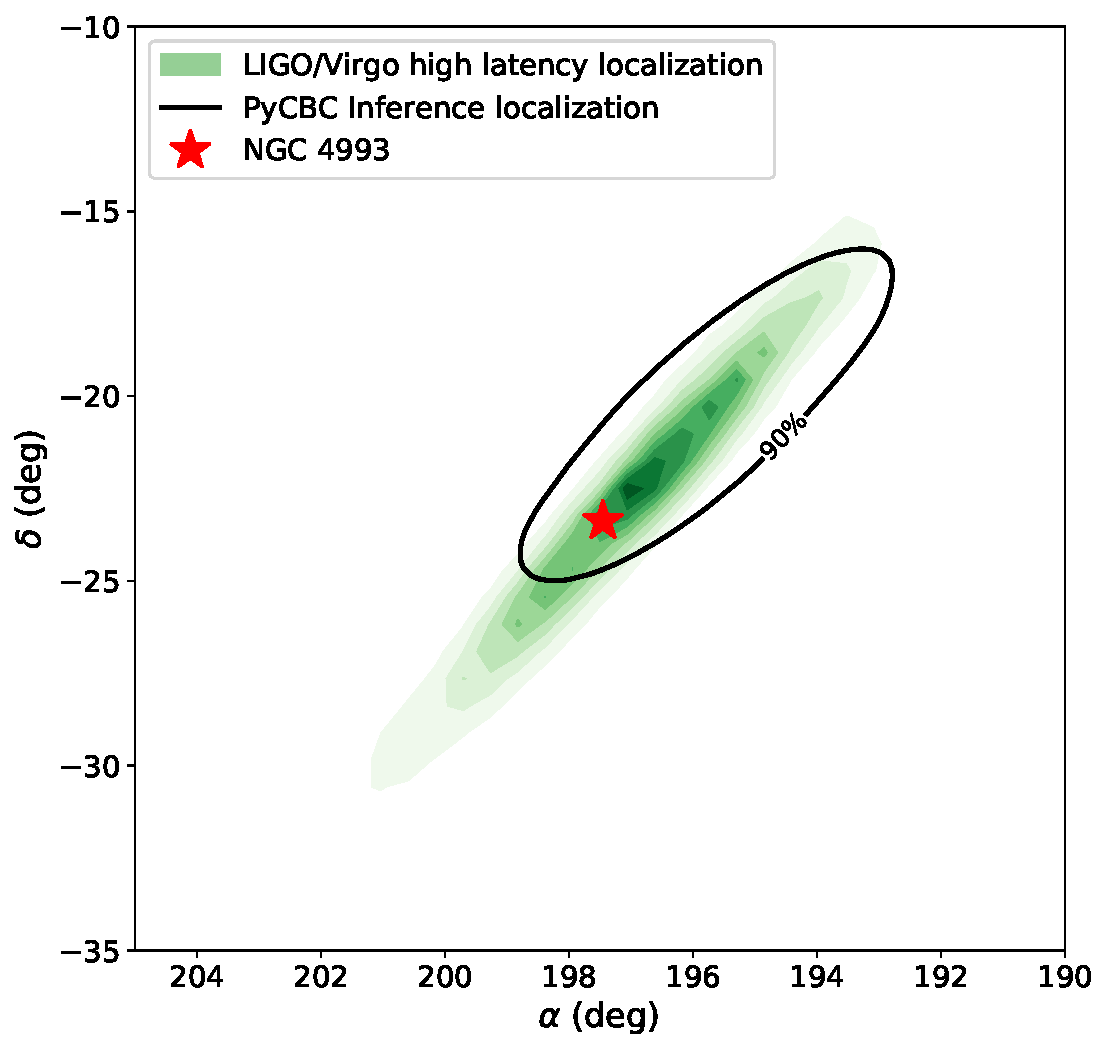
\includegraphics[width=\textwidth]{Figures/inc-angle/skyloc_comparison.pdf}
\caption{Sky localizations of GW170817 for LIGO/Virgo (green shaded region) and from our analysis using only GW source information (black contour). Both localizations are 90\% confidence regions, while the LIGO/Virgo region shows contours at each 10\% threshold. The location of NGC\,4993 is marked as a red star.}
\label{fig:skyloc}
\end{figure}

We then fix the sky location of GW170817 to R.A. = $197.450374^\circ$, decl. = $-23.381495^\circ$ \cite{Soares-Santos:2017lru} and remove these parameters from our parameter estimation.  Fixing the sky location of GW170817 has virtually no impact on the inclination measurement, in agreement with previous studies that have explored this correlation \cite{Seto:2005xb,Arun:2014ysa}. Finally, we set the prior probability distribution on the luminosity distance $p(d_L|H)$ to a Gaussian distribution centered on $40.7$ Mpc with a standard deviation of $2.36$ Mpc, corresponding to the measured distance and quadrature sum of statistical and systematic errors reported in \cite{Cantiello:2018ffy}. Here we have assumed a Gaussian distribution on this distance measurement, which we deem valid for a measurement of this precision and for the purpose of exploring upper and lower bounds.

\begin{figure}[ht]
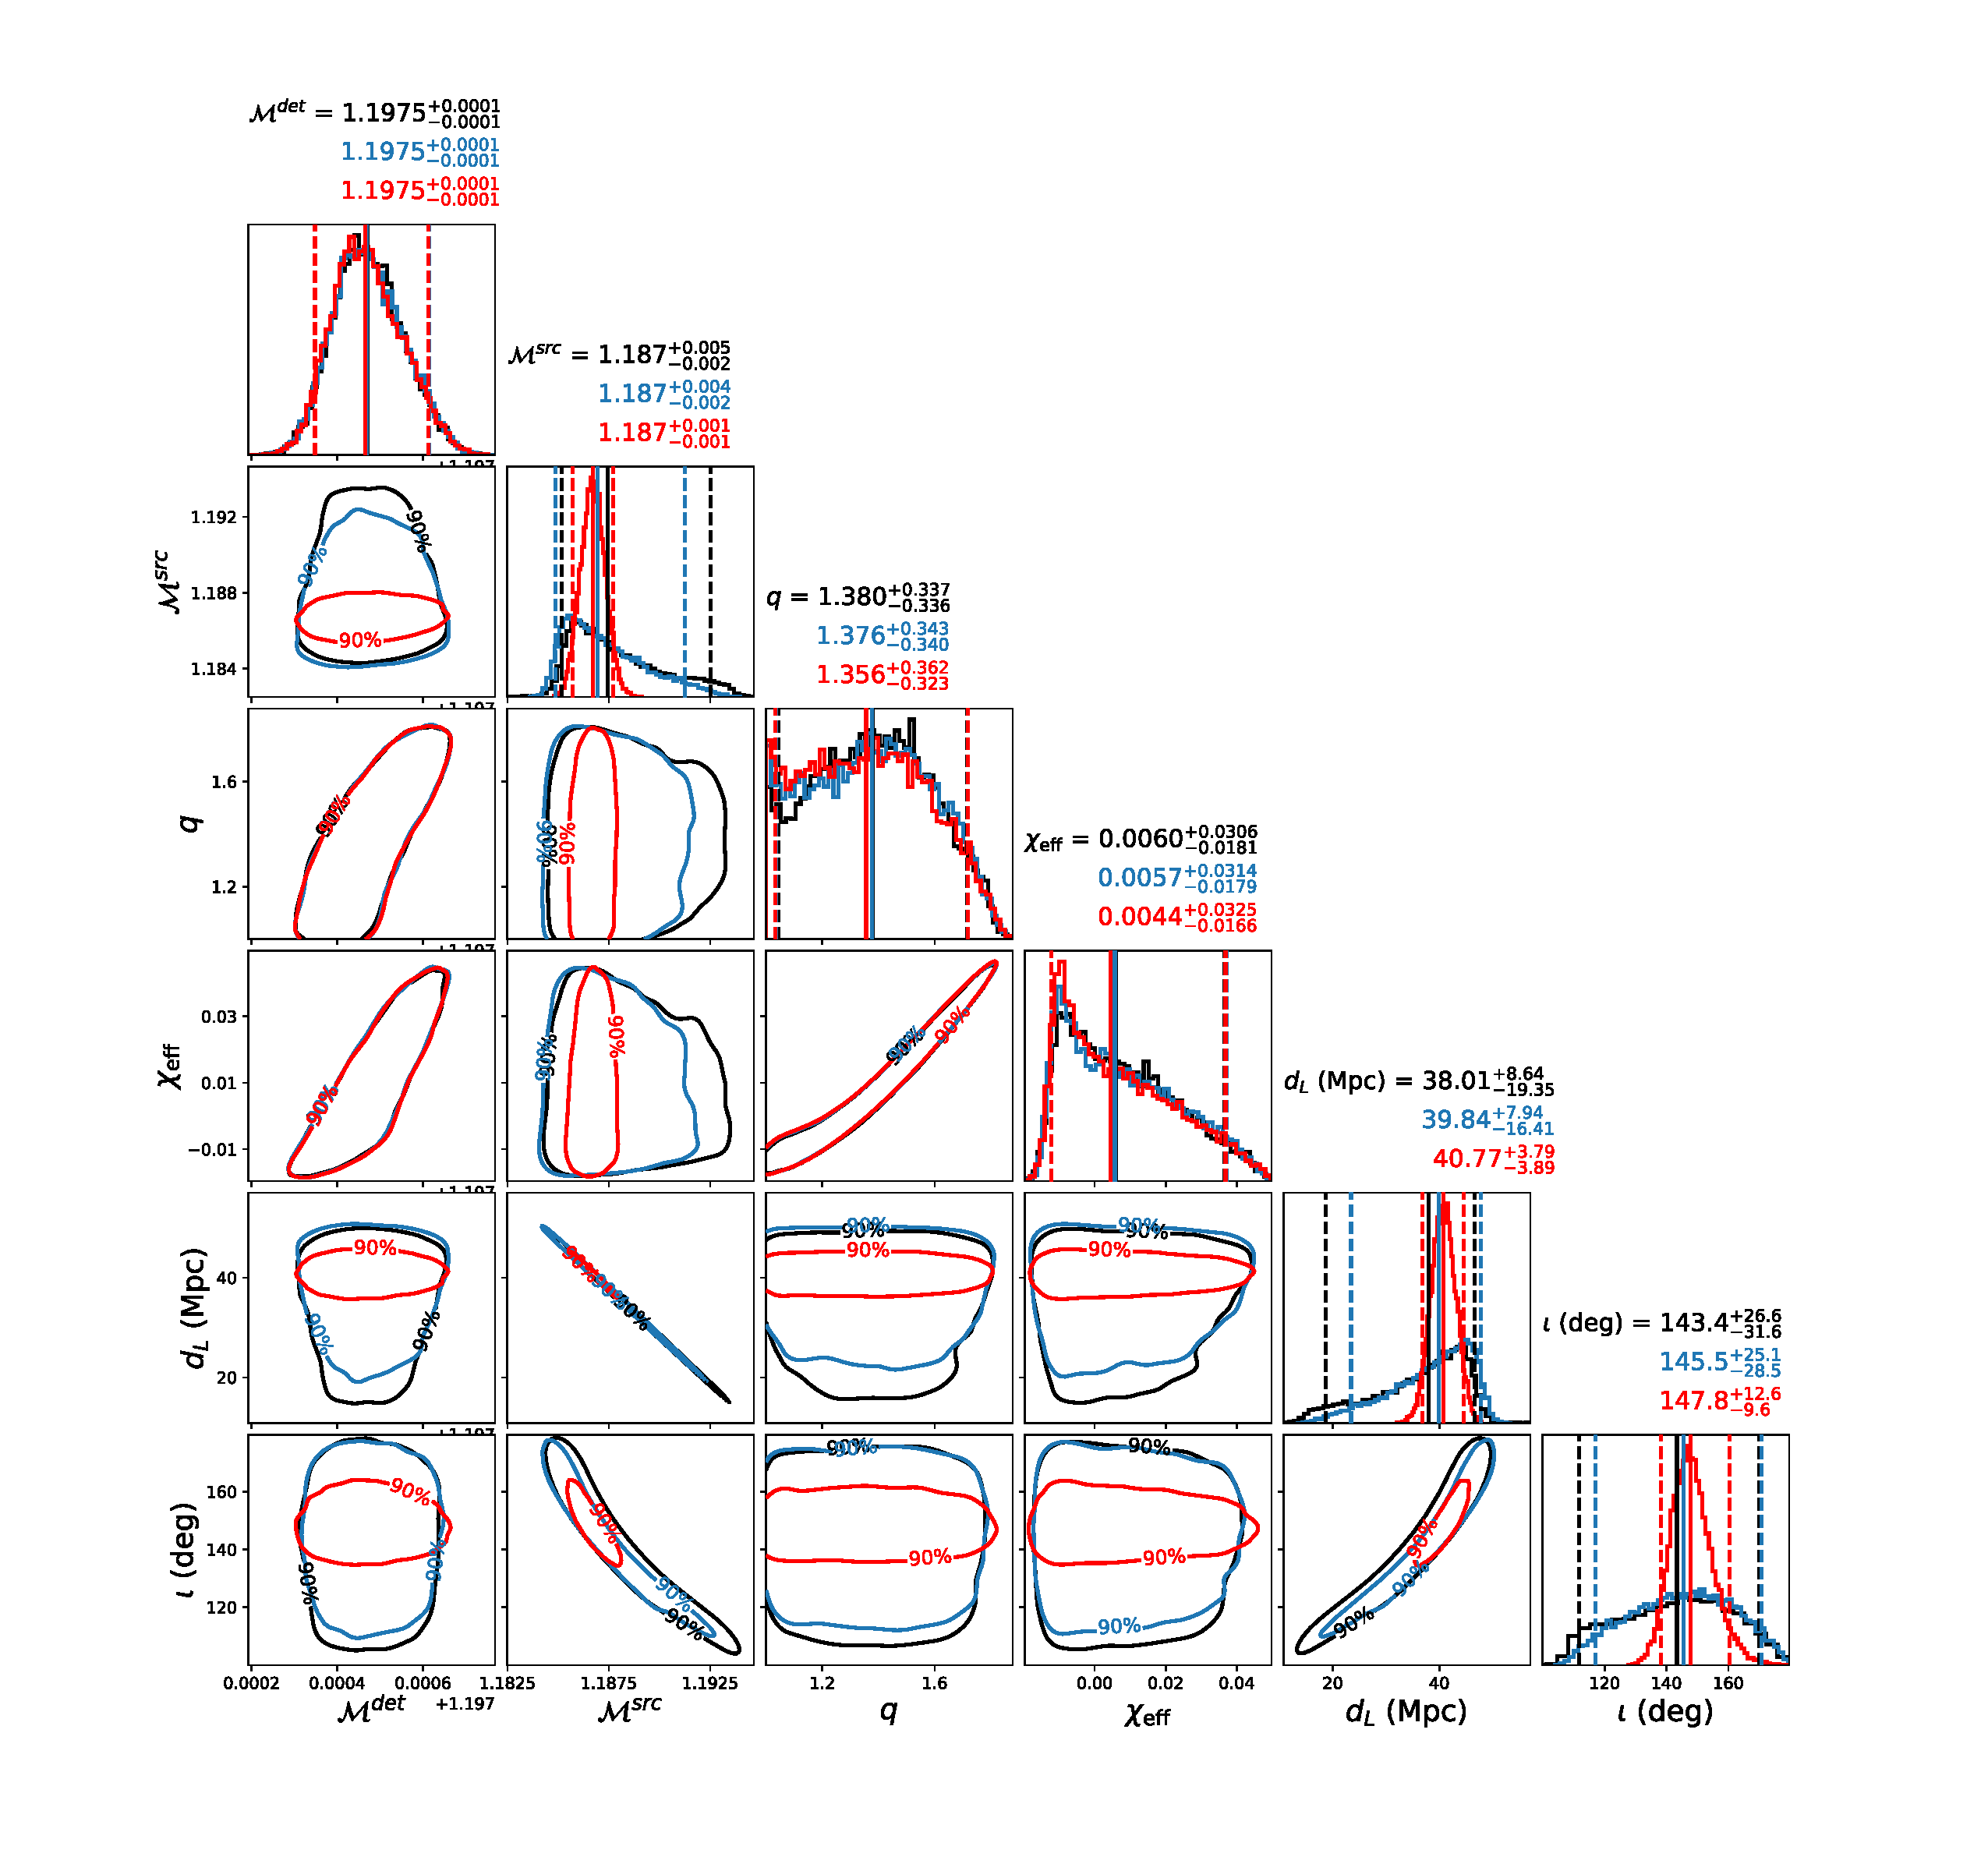
\includegraphics[width=\textwidth]{Figures/inc-angle/GW_vs_EM_pmspins_full_final.pdf}
\caption{Comparison of posterior probability distributions without and with combined EM information. The black contours show the results for using only the GW signal, the blue contours show the results for the fixed sky location of NGC\,4993, and the red contours show the results for both the fixed sky location and a Gaussian prior on distance of $40.7\pm 2.36$ Mpc from \cite{Cantiello:2018ffy}. These analyses used a prior on inclination angle that is uniform in $\cos \iota$. For each parameter, we quote the median value and the 90\% credible interval (shown with vertical solid and dashed lines, respectively, on the posterior plot of each parameter). The EM information on the distance measurement greatly improves the precision with which we measure the inclination angle (and significantly reduces the uncertainty on the source-frame chirp mass).}
\label{fig:posteriors}
\end{figure}

Using the EM observations as the prior on the luminosity distance results in significantly narrower posteriors on inclination angle and source-frame chirp mass $\mathcal{M} = (m_1 m_2)^{3/5}/(m_1 + m_2)^{1/5}$ shown in Figure~\ref{fig:posteriors}. The improved chirp mass measurement is due to the reduced error on $d_L$, as the $d_L$ posterior samples are used to convert from the measured detector-frame chirp mass $\mathcal{M}^\mathrm{det}$ to the source-frame chirp mass $\mathcal{M}^\mathrm{src}$ \cite{Schutz:1986gp,Finn:1992xs}. However, the improved precision on distance has no effect on our measurements of the component masses or spins, because at leading order the mass ratio $q = m_1/m_2$ and spin parameter $\chi_\mathrm{eff}$ \cite{Cutler:1994ys} are not correlated with distance. With the EM observations as the prior on $d_L$ and a prior on the inclination angle uniform in $\cos\iota$, we find that the viewing angle is $\Theta = 32^{+10}_{-13}$ degrees (90\% confidence).

Errors in the calibration of the GW detectors can cause errors in the measured amplitude of the GW signal and hence in the inclination angle of the binary. We treat this as a systematic error, which we measure by shifting the amplitude calibration of the LIGO and Virgo detectors by the 1$\sigma$ uncertainty bounds for LIGO/Virgo's second observing run \cite{Cahillane:2017vkb}. We find that shifting the calibration to its most sensitive and least sensitive extremes results in a $\pm 1.7^\circ$ shift in the peak of the viewing angle when using a prior on inclination angle that is uniform in $\cos \iota$. We quote this shift as the systematic error on our measurement. Changing the phase error of the calibration within the bounds reported in \cite{Cahillane:2017vkb} produces a negligible effect on the inclination angle.

A prior uniform in $\cos\iota$ goes to zero as the viewing angle approaches face on (or face off), so we repeat our analysis using a prior uniform in $\iota$. Figure~\ref{fig:inc} shows a comparison between the prior and the posterior distributions on inclination angle for each choice of prior. The result using a prior uniform in $\iota$ excludes viewing angles $\Theta \le 14.8^\circ$ at 90\% confidence, suggesting that our likelihood is indeed informative at small viewing angles and the lack of posterior support is not due to the prior uniform in $\cos\iota$ vanishing for small angles. Including the systematic error from calibration uncertainty, we set a conservative constraint of $\Theta \ge 13^\circ$ at 90\% confidence. This is consistent with the 10-day interval between the merger and the first observation of X-ray afterglow \cite{Troja:2017nqp}, which suggests that the GRB is not beamed at the Earth \cite{Guidorzi:2017ogy}.

\begin{figure}[ht]
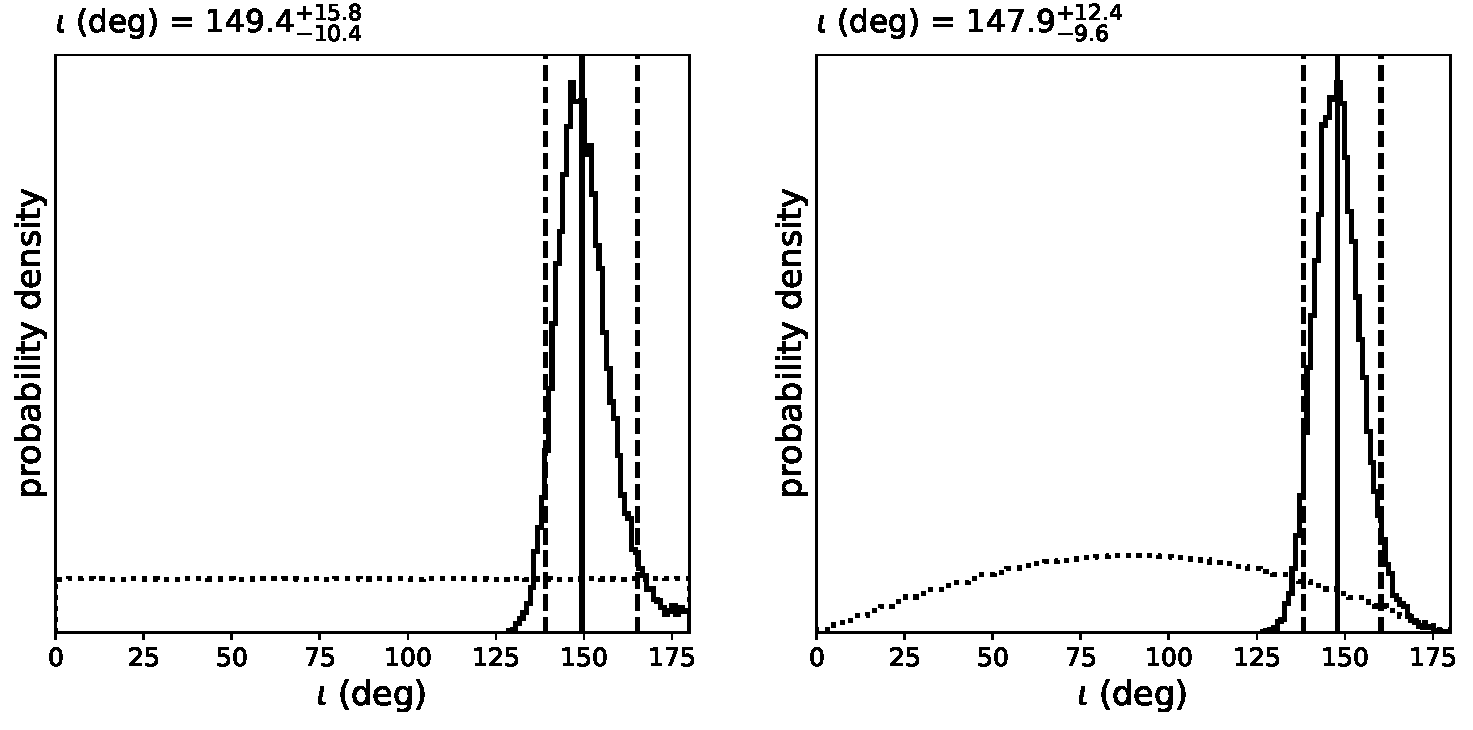
\includegraphics[width=\textwidth]{Figures/inc-angle/inc_post_vs_prior.pdf}
\caption{Inclination angle posteriors (solid lines) plotted against their prior (dotted lines) for two choices of prior: uniform in $\iota$ (left), and uniform in $\cos \iota$ (right). We quote the median value and the 90\% credible interval for $\iota$ in each posterior (shown with vertical lines). The prior uniform in $\cos \iota$ is the prior used by the LIGO/Virgo analysis. The uniform prior does not bias measurement away from angles approaching $180^\circ$, so these results suggest that our likelihood is informative close to $\iota = 180^\circ$ and that we can place a conservative lower bound on the viewing angle $\Theta \ge 13^\circ$ (90\% confidence).}
\label{fig:inc}
\end{figure}

\section{Discussion} \label{sec:disc}

Our joint GW--EM analysis of GW170817 used the GW observations along with sky location and a prior on the distance from direct measurement of these parameters from EM observations of NGC\,4993. Our 90\% confidence region on the viewing angle, $\Theta = 32^{+10}_{-13}\, \pm 1.7$ degrees (statistical and systematic errors), is significantly narrower than the inference made by GW observations alone, by about a factor of $2.6$.  It extends well above the $\Theta < 28^\circ$ bound of \cite{Mandel:2017fwk}, which was based on an assumed Hubble flow velocity for NGC\,4993. The precise distance measurement from \cite{Cantiello:2018ffy} also allows us to place a 90\% confidence lower bound on $\Theta$ that is substantially higher than the 68\% confidence lower bound, $\Theta > 10^\circ$, reported by \cite{Mandel:2017fwk}. 

Our improved constraint on $\Theta$ has implications for models of the prompt $\gamma$-ray and radio/X-ray afterglow emission from GW170817.  For example, our inferred value is in good agreement with the structured jet models of \cite{Lazzati:2017zsj}, which favor a viewing angle of $\approx 33^\circ$, and \cite{Margutti:2018xqd}, which favor a viewing angle of $\approx 20^\circ$.  While we do not yet know from a single event if the ejecta components that dominate the early UV/optical/near-infrared emission are significantly asymmetric, our constraint on $\Theta$ for GW170817 and future mergers will serve to shed light on the ejecta structure (e.g., spherical vs.~polar vs.~equatorial).




\Chapter{Fast Parameter Estimation of Binary Mergers for Multimessenger Followup}
\label{ch:rel-bin-pe}
Significant human and observational resources have been dedicated to electromagnetic followup of gravitational-wave events detected by Advanced LIGO and Virgo. As the sensitivity of LIGO and Virgo improves, the rate of sources detected will increase. \cite{Margalit:2019dpi} have suggested that it may be necessary to prioritize observations of future events. Optimal prioritization requires a rapid measurement of a gravitational-wave event's masses and spins, as these can determine the nature of any electromagnetic emission. We extend the relative binning method of \cite{cornish2013fast} and \cite{Zackay:2018qdy} to a coherent detector-network statistic. We show that the method can be seeded from the output of a matched-filter search and used in a Bayesian parameter measurement framework to produce marginalized posterior probability densities for the source's parameters within 20 minutes of detection on 32 CPU cores. We demonstrate that this algorithm produces unbiased estimates of the parameters with the same accuracy as running parameter estimation using the standard gravitational-wave likelihood. We encourage the adoption of this method in future LIGO-Virgo observing runs to allow fast dissemination of the parameters of detected events so that the observing community can make best use of its resources.

\section{Introduction}
The observation of the binary neutron star merger GW170817 in gravitational and electromagnetic waves \cite{TheLIGOScientific:2017qsa,GBM:2017lvd} has demonstrated the importance of multimessenger astronomy in answering fundamental questions in physics, astronomy, and cosmology; see e.g.~\cite{Monitor:2017mdv}, \cite{Lattimer:2019iye}, and \cite{Abbott:2017xzu}. With the observation of GW190814, gravitational-wave astronomy has begun to explore the properties of compact objects that are more massive than previously observed neutron stars and less massive than previously observed black holes~\cite{Abbott:2020khf}. Advanced LIGO and Virgo perform a search for compact-object binary mergers with several low-latency analyses based on matched filtering \cite{Messick:2016aqy,Nitz:2018rgo} and release alerts to the astronomical community to enable followup of detected events. As the sensitivity of the Advanced LIGO and Virgo detectors improves, the rate at which interesting events are detected will increase. \cite{Margalit:2019dpi} have suggested that it may become necessary to prioritize events for followup in future LIGO-Virgo observing runs. Optimal prioritization will require the knowledge of the source-frame component masses and spins of the binary, as these determine the type of electromagnetic counterpart that may be generated by the merger \cite{Foucart:2018rjc,Capano:2019eae}.

In this paper, we demonstrate that it is possible to perform full Bayesian parameter estimation on binary neutron star and neutron star--black holes signals within 20 minutes of the source's detection by  a matched-filter search (with an average time of 10.8 minutes) using  32 CPU cores (2.3~GHz Xeon\textsuperscript{\textregistered} Gold 6140). Our analysis produces marginalized posterior probability densities for the source's parameters (including source-frame masses, spins, sky location, and distance) that can be used to guide the prioritization of electromagnetic followup in future LIGO-Virgo observing runs. We achieve this by extending the relative binning method originally introduced by \cite{cornish2013fast} (and independently developed by \cite{Zackay:2018qdy}) to a fully coherent statistic, seeding the relative binning algorithm from the output of a matched-filter search, and using the \texttt{dynesty} nested-sampling package \cite{Speagle_2020}. We have made our code available in the PyCBC Inference framework \cite{Biwer:2018osg}.

We validate our analysis on a population of simulated binary neutron star and neutron star--black hole signals in a LIGO-Virgo detector network. A matched-filter search is used to identify signals that have a false alarm rate better than one per month. We then use our algorithm to produce marginalized posterior probability densities for each qualifying signal. For the parameters of interest, we perform a percentile-percentile test and demonstrate that our method produces unbiased parameter estimates. Comparing our sky localization to that of the \texttt{Bayestar} algorithm \cite{Singer_2016}, we find that the 90\% credible localization area improves by an average of 14 deg$^2$. We find that our analysis can recover the source-frame chirp mass to an accuracy of $\sim 5 \times 10^{-2}\msun$ for binary neutron star signals and $\sim 10^{-1}\msun$ for neutron star--black hole signals. We demonstrate that the measurement of mass ratio and spin is consistent with that of parameter estimation using the full likelihood, although these quantities are measured less accurately than the chirp mass as they enter the gravitational waveform at higher order and suffer from a partial degeneracy \cite{Cutler:1994ys,Hannam_2013}. As an example use case, we demonstrate that our method recovers essentially the same posterior probabilities for the parameters of GW170817 as the full likelihood calculation. Our method obtains marginalized posteriors for GW170817 in 20 minutes, compared to over three hours using the standard likelihood calculation.

This Letter is organized as follows: In Section \ref{sec:search} we describe our simulated search. Section \ref{sec:rel_bin_pe} describes our parameter estimation analysis and our implementation of relative binning for a detector network. Section \ref{sec:rel_bin_results} present our results including analysis run times and parameter estimation accuracy. Finally, we contrast our results to current methods in Section \ref{sec:rel_bin_conclusion}.

\section{Simulated Search}\label{sec:search}
We simulate a three-detector network representing the LIGO Hanford, LIGO Livingston \cite{TheLIGOScientific:2016agk,Buikema:2020dlj}, and Virgo \cite{TheVirgo:2014hva} detectors. We generate two populations of simulated signals: 600 binary neutron star and 570 neutron star--black hole binaries. Each population is injected into a realization of 33 hours of simulated detector data, which is created by coloring Gaussian noise to the design power spectral density of each detector \cite{Aasi:2013wya}. The simulated binary neutron star signals have their chirp mass drawn uniformly from the interval $[0.5, 3]~\msun$ and mass ratio $q=m_1/m_2$ drawn uniformly from the interval $[1, 3]$, with constraints on the component masses so that $1 < m_{1,2}/\msun < 3$. The neutron star's spins are restricted to be aligned with the orbital angular momentum and have dimensionless magnitude drawn uniformly from the interval $[-0.05, 0.05]$. The simulated neutron star--black hole signals have their chirp mass drawn uniformly from the interval $[0.5, 7]~\msun$ and mass ratio drawn uniformly from the interval $[1, 10]$, with constraints on the component masses so that $1 < m_{1,2}/\msun < 10$. Both component spins are restricted to be aligned with the orbital angular momentum, with the black hole spin dimensionless magnitude drawn uniformly from the interval $[-0.998, 0.998]$ and the neutron star spin dimensionless magnitude drawn uniformly from the interval $[-0.05, 0.05]$. This population of sources is chosen to cover the region in which it is expected that there will be neutron star disruption and an electromagnetic counterpart \cite{Capano:2019eae}. Each set of simulated signals is uniformly distributed in sky location and follow a uniform-in-volume distance distribution with $d_{L}\in[10, 300]$~Mpc for binary neutron star signals and $d_{L}\in[10, 500]$~Mpc for neutron star--black hole signals. This corresponds to a signal population with single-detector signal-to-noise ratios of $1$ to $O(100)$. Binary neutron star signals are simulated using the TaylorF2 waveform approximant~\cite{Dhurandhar:1992mw,Droz:1999qx,Blanchet:1995ez,Faye:2012we}. The neutron star--black hole signals are simulated using the IMRPhenomD approximant \cite{Husa:2015iqa,Khan:2015jqa}. For both populations, we set the tidal deformability of the neutron stars $\Lambda$ to zero, as this does not have a significant effect on the parameters we are investigating in this paper \cite{Damour:2012yf}.

To simulate the output of the LIGO-Virgo searches, we run each set of simulated signals through the PyCBC search pipeline \cite{Usman:2015kfa} configured to operate in a similar way to the PyCBC Live low-latency search used in the recent Advanced LIGO--Virgo observing runs \cite{DalCanton:2020vpm}. This search uses matched filtering \cite{Allen_2012} with a template bank of gravitational waveforms designed to give at least a 97\% match, measured by noise-weighted overlap, to any potential signal in the relevant parameter space \cite{DalCanton:2017ala,LIGOScientific:2018mvr}. The bank is designed to catch potentially electromagnetically-bright signals, and contains 315,325 waveforms. Template waveforms have component masses spanning [1, 30] $\msun$ and dimensionless spin magnitudes in the range [-1, 1], with the spin restricted to the direction of the orbital angular momentum. Templates in the bank are generated using the TaylorF2 approximant for signals with total mass $M=m_{1}+m_{2}< 4\msun$ \cite{Faye:2012we}, and with a reduced-order model of the SEOBNRv4 approximant otherwise \cite{Bohe:2016gbl}. Candidate triggers are required to be matched by the same template in at least two detectors in the network and with consistent phase, amplitude, and time of arrival given the network orientation and relative sensitivities between detectors \cite{Nitz:2017svb}. The search pipeline provides best-fit template parameters for every trigger and measures the trigger's statistical significance. The significance of a trigger is determined by the time-slide method and the pipeline computes a false alarm rate for each trigger. We select the triggers that have a false alarm rate more significant than 1 per month as candidate events for parameter estimation followup. This threshold was selected to be the same as that used to release low-latency events as public alerts for electromagnetic followup in the third LIGO-Virgo observing run \cite{emfollowdoc} and corresponds to a network signal-to-noise ratio of approximately $8.3$. Of the total injections made, 306 binary neutron star and 253 neutron star--black hole injections satisfied this threshold.

\section{Parameter estimation}\label{sec:rel_bin_pe}

We use \textit{PyCBC Inference} \cite{Biwer:2018osg} with the \texttt{dynesty} nested sampler \cite{Speagle_2020} to perform Bayesian parameter estimation on candidate events from the search pipeline. In general, under the assumption of Gaussian noise characterized by a power spectrum $S(f)$, the likelihood of obtaining detector data $d$ given the presence of a gravitational waveform $h(\theta)$ is
\begin{equation}
    \mathcal{L}(d|\theta)\propto\exp\left[-\frac{1}{2}\left<d-h(\theta)|d-h(\theta)\right>\right],
\end{equation}
where
\begin{equation}
    \left<a|b\right>=4\mathfrak{R}\int_{f_{\mathrm{min}}}^{f_{\mathrm{max}}}\frac{\tilde{a}^{*}(f)\tilde{b}(f)}{S(f)}df
\end{equation}
is the noise-weighted inner product \cite{Finn:1992xs,Chernoff:1993th}.
In evaluating this likelihood, we can obtain estimates of the gravitational-wave parameters $\theta$ through the posterior probability distribution
\begin{equation}
    p(\theta|d)\propto\mathcal{L}(d|\theta)p(\theta),
\end{equation}
where $p(\theta)$ is the assumed prior probability distribution of the parameters. To calculate the likelihood, we use the relative binning method of \cite{cornish2013fast} and \cite{Zackay:2018qdy}, which uses a linear interpolation across frequency samples over which the accumulated phase difference $\delta\phi$ between a fiducial waveform and nearby waveforms is less than a tunable threshold. This effectively downsamples the number of frequency points used to compute the likelihood, thereby speeding up the parameter estimation.

The implementation of relative binning used by \cite{Zackay:2018qdy} did not incorporate a coherent network detection statistic. We extend their method to include the extrinsic parameters which are needed to measure the sky location of an event: right ascension $\alpha$, declination $\delta$, geocentric time of coalescence $t_c$, inclination angle $\iota$, and gravitational-wave polarization angle $\psi$. These parameters are incorporated into the likelihood by projecting each template waveform onto the individual detectors in the network. A general frequency domain waveform template $h$ as seen by a detector can be written as
\begin{equation}
    h(f)=F_{+}(\alpha,\delta,\psi)h_{+}(f) + F_{\times}(\alpha,\delta,\psi)h_{\times}(f)
\end{equation}
where $h_{+,\times}$ are the plus and cross polarizations of the waveform, and $F_{+,\times}$ are the detector antenna responses to the two polarizations \cite{Anderson_2001}. The amplitude of the individual waveform polarizations depend on the inclination angle $\iota$ \cite{thorne.k:1987}
\begin{equation}
    h_{+}\propto \frac{1}{2}(1+\cos^{2}{\iota}),
\end{equation}
\begin{equation}
    h_{\times}\propto \cos{\iota}.
\end{equation}
We generate waveforms using both polarizations in order to capture this dependence. Similarly, we measure $\alpha$, $\delta$, $t_{c}$, and $\psi$ dependence through the detector antenna responses as the orientation of the detector arms, and thus the sensitivity to the two polarizations, will change as the Earth moves. To account for coherent network timing delays, we calculate detector-specific arrival times for each template waveform using $\alpha$, $\delta$, and $t_{c}$, based on the geometry of the network with respect to the source at the time of the signal, along with the light travel time from the Earth center \cite{Fairhurst:2009tc}.

The relative-binned likelihood calculation requires a fiducial waveform known to be near the peak of the likelihood. The chirp mass of the template used to generate a candidate by a search pipeline is accurate to within a few $10^{-3} \msun$ for binary neutron star signals \cite{Berry_2016,Biscoveanu_2019} and to approximately $1\%$ for neutron star--black hole signals \cite{canton2020realtime}. Since the chirp mass is the leading order parameter governing phase evolution for a binary inspiral \cite{Peters:1963ux}, the best-fit template will be near the peak of the likelihood. We therefore use the parameters that the search pipeline reports for a signal to generate the fiducial waveform that seeds the relative binning method. For the fiducial sky location, inclination, and polarization, we arbitrarily choose $\alpha_{f}=\pi$, $\delta_{f}=0$, $\iota_{f}=0$, and $\psi_{f}=\pi$, as we find that more accurate initial estimates are unnecessary to correctly recover the source parameters. The fiducial coalescence time is set to be the arithmetic mean of the coalescence time reported by the search pipeline for each detector.

Parameter estimation is performed over the detector-frame chirp mass $\mathcal{M}$, the mass ratio $q=m_{1}/m_{2},~m_{1}\ge m_{2}$, the component aligned spins $\chi_{1,2}$, the geocentric time of coalescence $t_{c}$, the inclination angle $\iota$, the right ascension $\alpha$, the declination $\delta$, the luminosity distance $d_{L}$, and the gravitational-wave polarization angle $\psi$. The likelihood calculation includes an analytic marginalization over the coalescence phase $\phi_{c}$. We use the TaylorF2 approximant to generate the likelihood for binary neutron star waveforms and the IMRPhenomD approximant for the neutron star--black hole waveforms. For all simulated signals we use a low-frequency cutoff of 30~Hz and a sample rate of 2048~Hz.

The prior distributions used in the parameter estimation are the same as those of the corresponding population of simulated signals for each parameter, with the exception of the chirp mass which we restrict to be uniform in $\mathcal{M} \in [\mathcal{M}_{s}-0.1, \mathcal{M}_{s}+0.1]~\msun$, where $\mathcal{M}_{s}$ is the chirp mass of the template reported by the search. This constraint on the chirp mass prior enables quicker convergence of the parameter estimation, but in all cases the restricted bounds are well outside the region of posterior support and so do not affect the accuracy of recovery.

For each simulated signal recovered with false alarm rate more significant than 1 per month by the search pipeline, we run the relative-binned parameter estimation analysis
to produce posterior distributions for the 10-dimensional set of waveform parameters $\theta = (\mathcal{M}, q, \chi_{1}, \chi_{2}, t_{c}, \iota, \alpha, \delta, d_{L}, \psi)$. For each signal, we measure the wall-clock time that it takes to perform the parameter estimation on 32 cores of an Intel\textsuperscript{\textregistered} Xeon\textsuperscript{\textregistered} Gold 6140 processor running at a clock speed of 2.3~GHz. 

\section{Results} \label{sec:rel_bin_results}

The timing results for the two simulated populations as a function of the network signal-to-noise ratio of the maximum likelihood template are shown in the left panel of Fig.~\ref{fig:timing_and_pp}. The average run time for a single signal is 10.8 minutes, with the maximum run-time being 20 minutes for all signals. The parallelization used by the nested sampling algorithm is saturated at approximately 32 cores, so while a small decrease in wall-clock time may be gained by fine-tuning the number of cores, increasing the number beyond 32 does not significantly decrease the run time. Processors with a faster clock speed will generally decrease run time, however.

\begin{figure}[b]
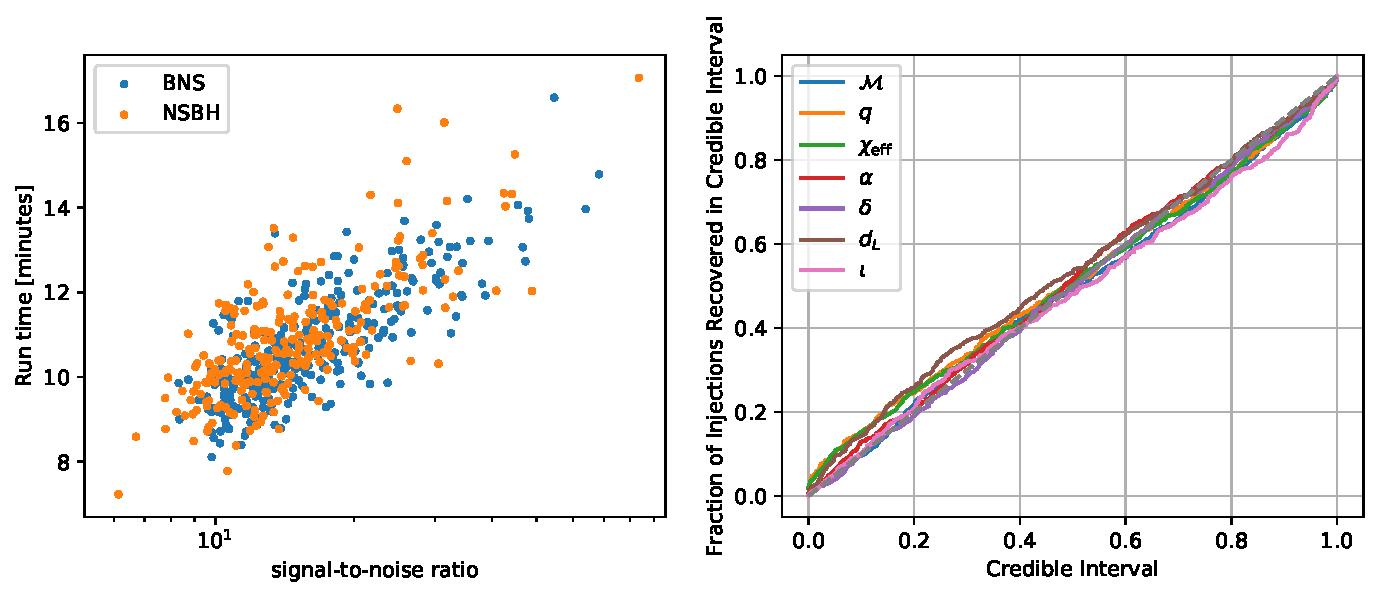
\includegraphics[width=\textwidth]{Figures/rel-bin-pe/timing_and_pp_plot.pdf}
\caption{\textit{Left:} The wall-clock time in minutes that it takes to perform the parameter estimation using the coherent relative binning likelihood and nested sampling on 32 cores of an Intel\textsuperscript{\textregistered} Xeon\textsuperscript{\textregistered} Gold 6140 processor running at a clock speed of 2.3~GHz as a function of the network signal-to-noise ratio of the maximum likelihood template. The average run-time for a single signal is 10.8 minutes, with the maximum run-time being 20 minutes for all signals. Increasing the number of cores does not significantly decrease the wall-clock run-time. The run-time shows a slight increase as a function of the signal-to-noise ratio, as expected given that signals with a larger signal-to-noise ratio have a more narrowly peaked likelihood. \textit{Right:} The fraction of injections recovered within a credible interval plotted as a function of credible interval. Fidelity to the 1:1 diagonal line is an indication of probability being uniformly distributed across a given parameter's posterior distribution and is a measure of the accuracy of this analysis at the population level. We find that all of the parameters of interest are estimated in an unbiased way by our parameter estimation method.}
\label{fig:timing_and_pp}
\end{figure}

To determine whether our method of measuring the parameters is accurate for the population of injected signals, we perform a percentile-percentile (PP) test on each of the main parameters of interest: chirp mass $\mathcal{M}$, mass ratio $q$, effective spin $\chi_{\mathrm{eff}}=(m_{1}\chi_{1}+m_{2}\chi_{2})/(m_{1}+m_{2}$, right ascension $\alpha$, declination $\delta$, luminosity distance $d_L$, and inclination $\iota$. The PP test calculates the distribution of percentile ranks for all injected parameter values within their respective posteriors and constructs the fraction of injections recovered within a credible interval as a function of credible interval. Any deviation from uniformity in this distribution for a parameter is an indication of measurement bias. We measure any deviation with the Kolmogorov-Smirnov (KS) test \cite{10.2307/2280095}, which computes the distance between the empirical distribution that we find for the PP test and the expected distribution. The results of the PP tests are shown in the right panel of Fig.~\ref{fig:timing_and_pp}. For every parameter of interest, we find that the PP test follows the ideal distribution well, with the KS test indicating that the percentile rank distributions cannot be meaningfully distinguished from uniform. Our results show that our analysis produces unbiased estimates for each of the parameters of interest.

To examine the accuracy of sky localization, we calculate the area on the sky containing 90\% of the probability for the location of the source. We compare the area of this probability contour to the 90\% credible interval of the sky-map produced in low-latency by the \texttt{Bayestar} algorithm \cite{Singer_2016}. Fig.~\ref{fig:localization} shows the cumulative fraction of signals recovered as a function of the 90\% confidence localization area for our method and by \texttt{Bayestar}. For direct comparison to the results of \cite{Singer_2016}, we calculate the cumulative fraction using all recovered signals, and the subset of the recovered signals that is detected above threshold in all three detectors.  We find that the area of the 90\% credible region improves by an average of 14 deg$^2$ when using the relative binning parameter estimation compared to \texttt{Bayestar}.

\begin{figure}[ht]
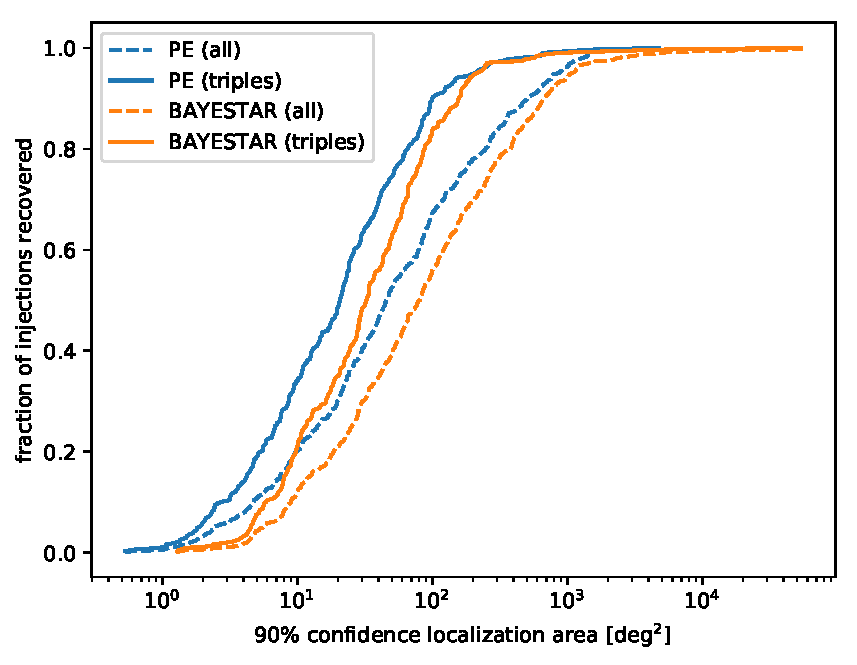
\includegraphics[width=\textwidth]{Figures/rel-bin-pe/localization_cumulative_allinj_eps0p03.pdf}
\caption{Fraction of injections recovered as a function of the 90\% confidence localization area. The localization results from our parameter estimation analysis are shown in blue, and those from the \texttt{Bayestar} algorithm are in orange. The dotted lines show the results for the entire set of signals, while solid lines show only signals that were above the detection threshold in all three detectors in our simulated search. We find our localization areas are consistently smaller than those from \texttt{Bayestar}, as indicated by the blue lines lying to the left of the orange lines, although the difference in areas is not large. The improvement in localization area between \texttt{Bayestar} and our analysis is 14 deg$^2$ on average, and is comparable between the set of triple-coincident signals and the set of all signals.}
\label{fig:localization}
\end{figure}

To examine the accuracy of parameter recovery, we calculate the difference between the median of the posterior and the known injected value for each parameter. The accuracy of chirp mass recovery in the source-frame is shown in the top panels of Fig.~\ref{fig:residuals_and_uncertainty} as a function of the network signal-to-noise ratio for each recovered signal. As expected, the accuracy of recovery increases as the signal-to-noise increases. For binary neutron star signals the difference between the median value of the chirp mass posterior and the injected value is less than $\sim 5 \times 10^{-2}\msun$ for all simulated signals. This accuracy improves by a factor of $2$ for signal-to-noise greater than $20$. Neutron star--black hole signals generally have larger uncertainties on their parameters and we find chirp mass residuals for these signals to be less than $10^{-1}\msun$ for signal-to-noise greater than $10$ and a factor of $2$ less than that for signal-to-noise greater than $20$. For comparison, we show the accuracy of the source-frame chirp mass of the best-fit template from the search. The search measures the detector-frame parameters of the gravitational-wave signal, so we convert this to the source-frame by computing the redshift at the median distance reported by \texttt{Bayestar} for the candidate event. The accuracy of the best-fit chirp mass from the search is an order of magnitude worse than estimated by \cite{Biscoveanu_2019}. However, the majority of the error comes from the calculation of the source-frame chirp mass. Comparing the detector-frame chirp mass of the simulated signal to the best-fit template, we find errors of $\sim 10^{-3}\msun$. While the accuracy of the best-fit template degrades for quieter signals, using this  estimate as a seed for the relative-binned analysis does not affect the recovery of the source parameters.

The middle row of Fig.~\ref{fig:residuals_and_uncertainty} shows the fractional uncertainty in the chirp mass $\sigma_\mathcal{M} / \langle \mathcal{M} \rangle$, where $\sigma_\mathcal{M}$ and $\langle \mathcal{M} \rangle$ are the standard deviation and mean of the posterior distribution. By this measure we find the accuracy of our method for the binary neutron star population is comparable to that of \cite{Farr:2015lna}. As an additional check we also run parameter estimation using the full likelihood for a subset of the population and find that the accuracy of the relative binning method is consistent with results using the full likelihood for both binary neutron star and neutron star--black hole signals. These results show that our recovery of the chirp mass for all signals has more than sufficient accuracy to determine the expected type of electromagnetic counterpart and the possible fate of the merger remnant using the method of \cite{Margalit:2019dpi}.

\begin{figure}[ht]
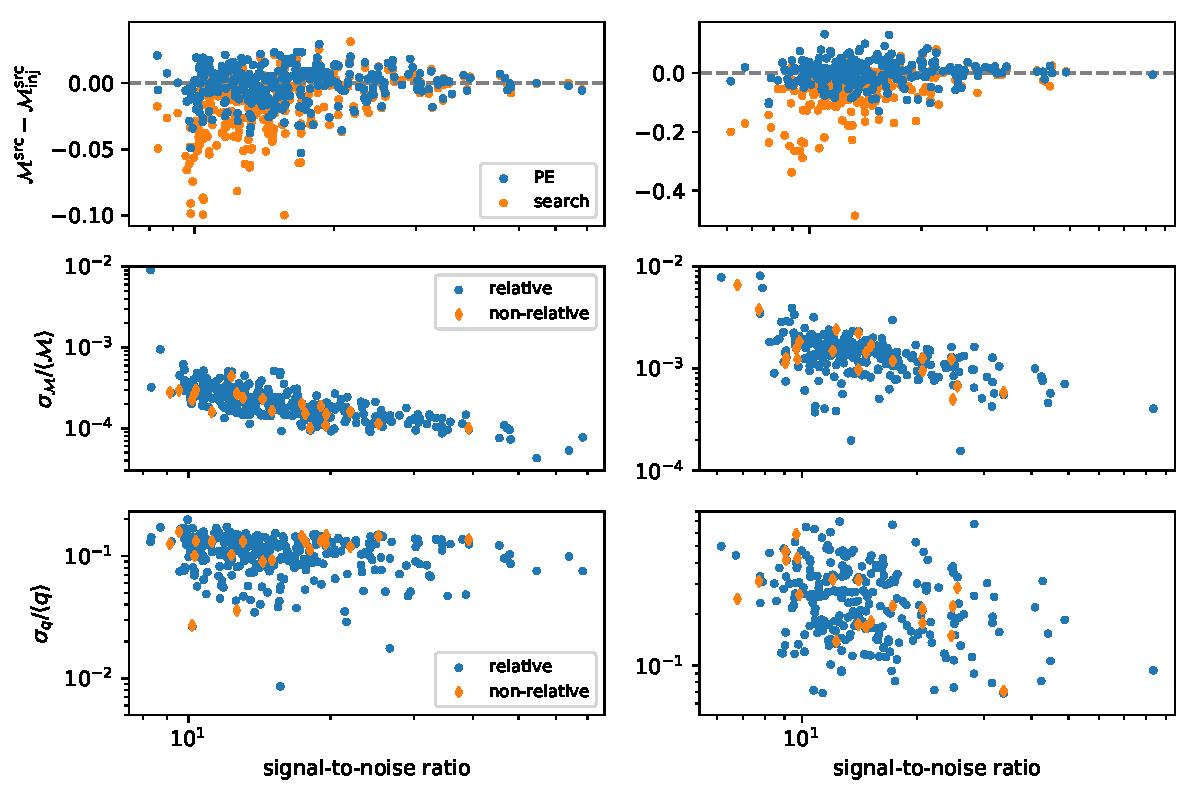
\includegraphics[width=\textwidth]{Figures/rel-bin-pe/residuals_and_frac_uncertainty_6panel.pdf}
\caption{Chirp mass and mass ratio recovery metrics for the binary neutron star (left column) and neutron star--black hole (right column) signals in our analysis. \textit{Top row:} Difference between source-frame chirp mass estimates and the true injected value, as a function of signal-to-noise ratio. Blue circles denote differences from the median posterior values from parameter estimation, while orange circles show differences from best-fit template values from the search. We find that on average our parameter estimation results improve on the accuracy of the best-fit template by a factor of $2$. \textit{Middle and bottom rows:} Fractional uncertainties on chirp mass and mass ratio, respectively, calculated as the ratio of standard deviation and mean of the posterior distributions. Uncertainties from our relative-binned analysis are shown as blue circles, and those from a standard non-relative likelihood analysis on a subset of the population are shown as orange diamonds. Our relative-binned results are consistent with the non-relative analysis, and also with the results in \cite{Farr:2015lna}.}
\label{fig:residuals_and_uncertainty}
\end{figure}

The gravitational-wave phase evolution is less sensitive to changes in the mass ratio  and so the component masses of the binary are less well recovered than the chirp mass \cite{Cutler:1994ys}. A degeneracy exists between the mass ratio and component spins of the binary which makes measuring the component masses and spins challenging, especially for neutron star--black hole systems \cite{Hannam_2013}. The bottom row of Fig.~\ref{fig:residuals_and_uncertainty} shows the accuracy of measuring the mass ratio $q = m_1/m_2$. Although the measurement of this parameter is less accurate than that of the chirp mass, our results are again comparable to those seen by \cite{Farr:2015lna} and they are consistent with our comparison analysis using the full likelihood on a subset of the population. This demonstrates that the reduced accuracy is intrinsic to the measurability of the parameter and not a result of using the relative binning algorithm.

To further illustrate the utility of our method in recovering parameters of interest to the observing community, Fig.~\ref{fig:component_recovery} shows the source-frame component mass residuals for all signals as well as the black hole spin residuals for the neutron star--black hole signals, plotted as a function of the network signal-to-noise ratio. The binary neutron star component masses are shown in the left panels of the figure. The residuals on the primary mass are generally less than about $0.5\msun$ with only a slight tendency to smaller values as signal-to-noise increases. The secondary mass residuals are somewhat smaller, less than about $0.3\msun$, which can be attributed to the relatively narrow mass parameter space ($1-3\msun$) and our convention requiring $m_{2}<m_{1}$.

\begin{figure}[ht]
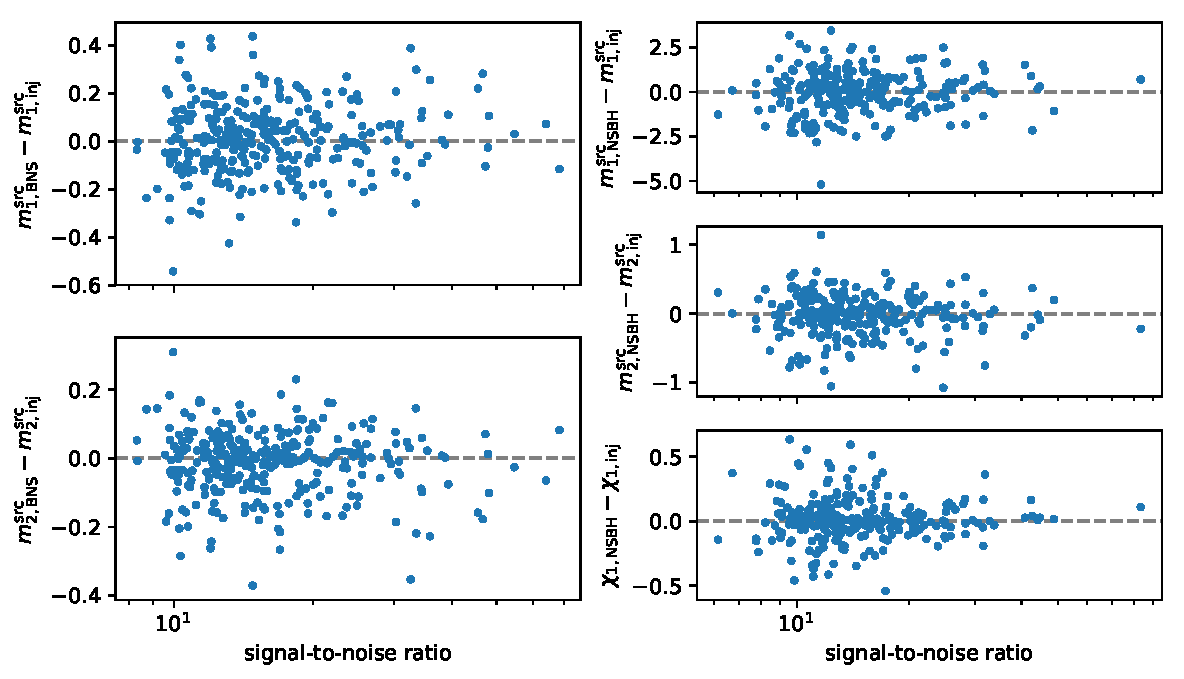
\includegraphics[width=\textwidth]{Figures/rel-bin-pe/component_residuals_src_frame_2col.pdf}
\caption{Difference between parameter estimates and true injected values for some component parameters of interest, plotted against signal-to-noise ratio. The left column shows results for the component masses of binary neutron star signals, and the right column shows results for the component masses and black hole spin of neutron star--black hole signals. Differences are computed from median posterior values, and masses have been converted to the source-frame using the distance posteriors. We find both component masses of binary neutron star signals are generally constrained to within $\sim 0.5\msun$ of the true value for all signals, while the majority of primary and secondary masses of neutron star--black hole signals are within about $3\msun$ and $1\msun$ respectively. We find our black hole spin measurements are uninformative below a signal-to-noise of $20$, but for louder signals the spin is within about $0.3$ of the true value.}
\label{fig:component_recovery}
\end{figure}

Neutron star--black hole signals have larger uncertainties on their intrinsic parameter estimates owing to the larger mass and spin parameter space and the known degeneracy between mass ratio and spin \cite{Hannam_2013}. However, these quantities are important in determining whether a merger will produce an electromagnetic counterpart. The residuals on component masses and black hole spin for our neutron star--black hole signals are shown in the right panels of Fig.~\ref{fig:component_recovery}. We find the primary and secondary mass residuals are mostly less than $3\msun$ and $1\msun$, respectively. Our estimates of the black hole spin are generally uninformative below a signal-to-noise of $20$, but above this threshold we find the residuals are constrained to be less than $\sim 0.3$.

As a final example of the effectiveness of our method, we apply it to GW170817 \cite{TheLIGOScientific:2017qsa} without including any prior knowledge of host galaxy location or distance. For comparison, we also repeat the analysis using a standard non-relative likelihood, and the posteriors from both runs are shown in Fig.~\ref{fig:gw170817_comparison}. For all measured parameters, we find the posterior distributions from the relative and non-relative analyses are nearly identical, in agreement with \cite{Dai:2018dca}. However, the analysis using the relative binning likelihood seeded by a search took only 20 minutes to complete, as compared to over 3 hours for the standard likelihood computation. In the only confirmed observation of a multimessenger gravitational-wave source to date, our analysis is able to provide the same localization region as the standard likelihood as well as the same intrinsic parameter estimates in substantially less computational time.

\begin{figure}[ht]
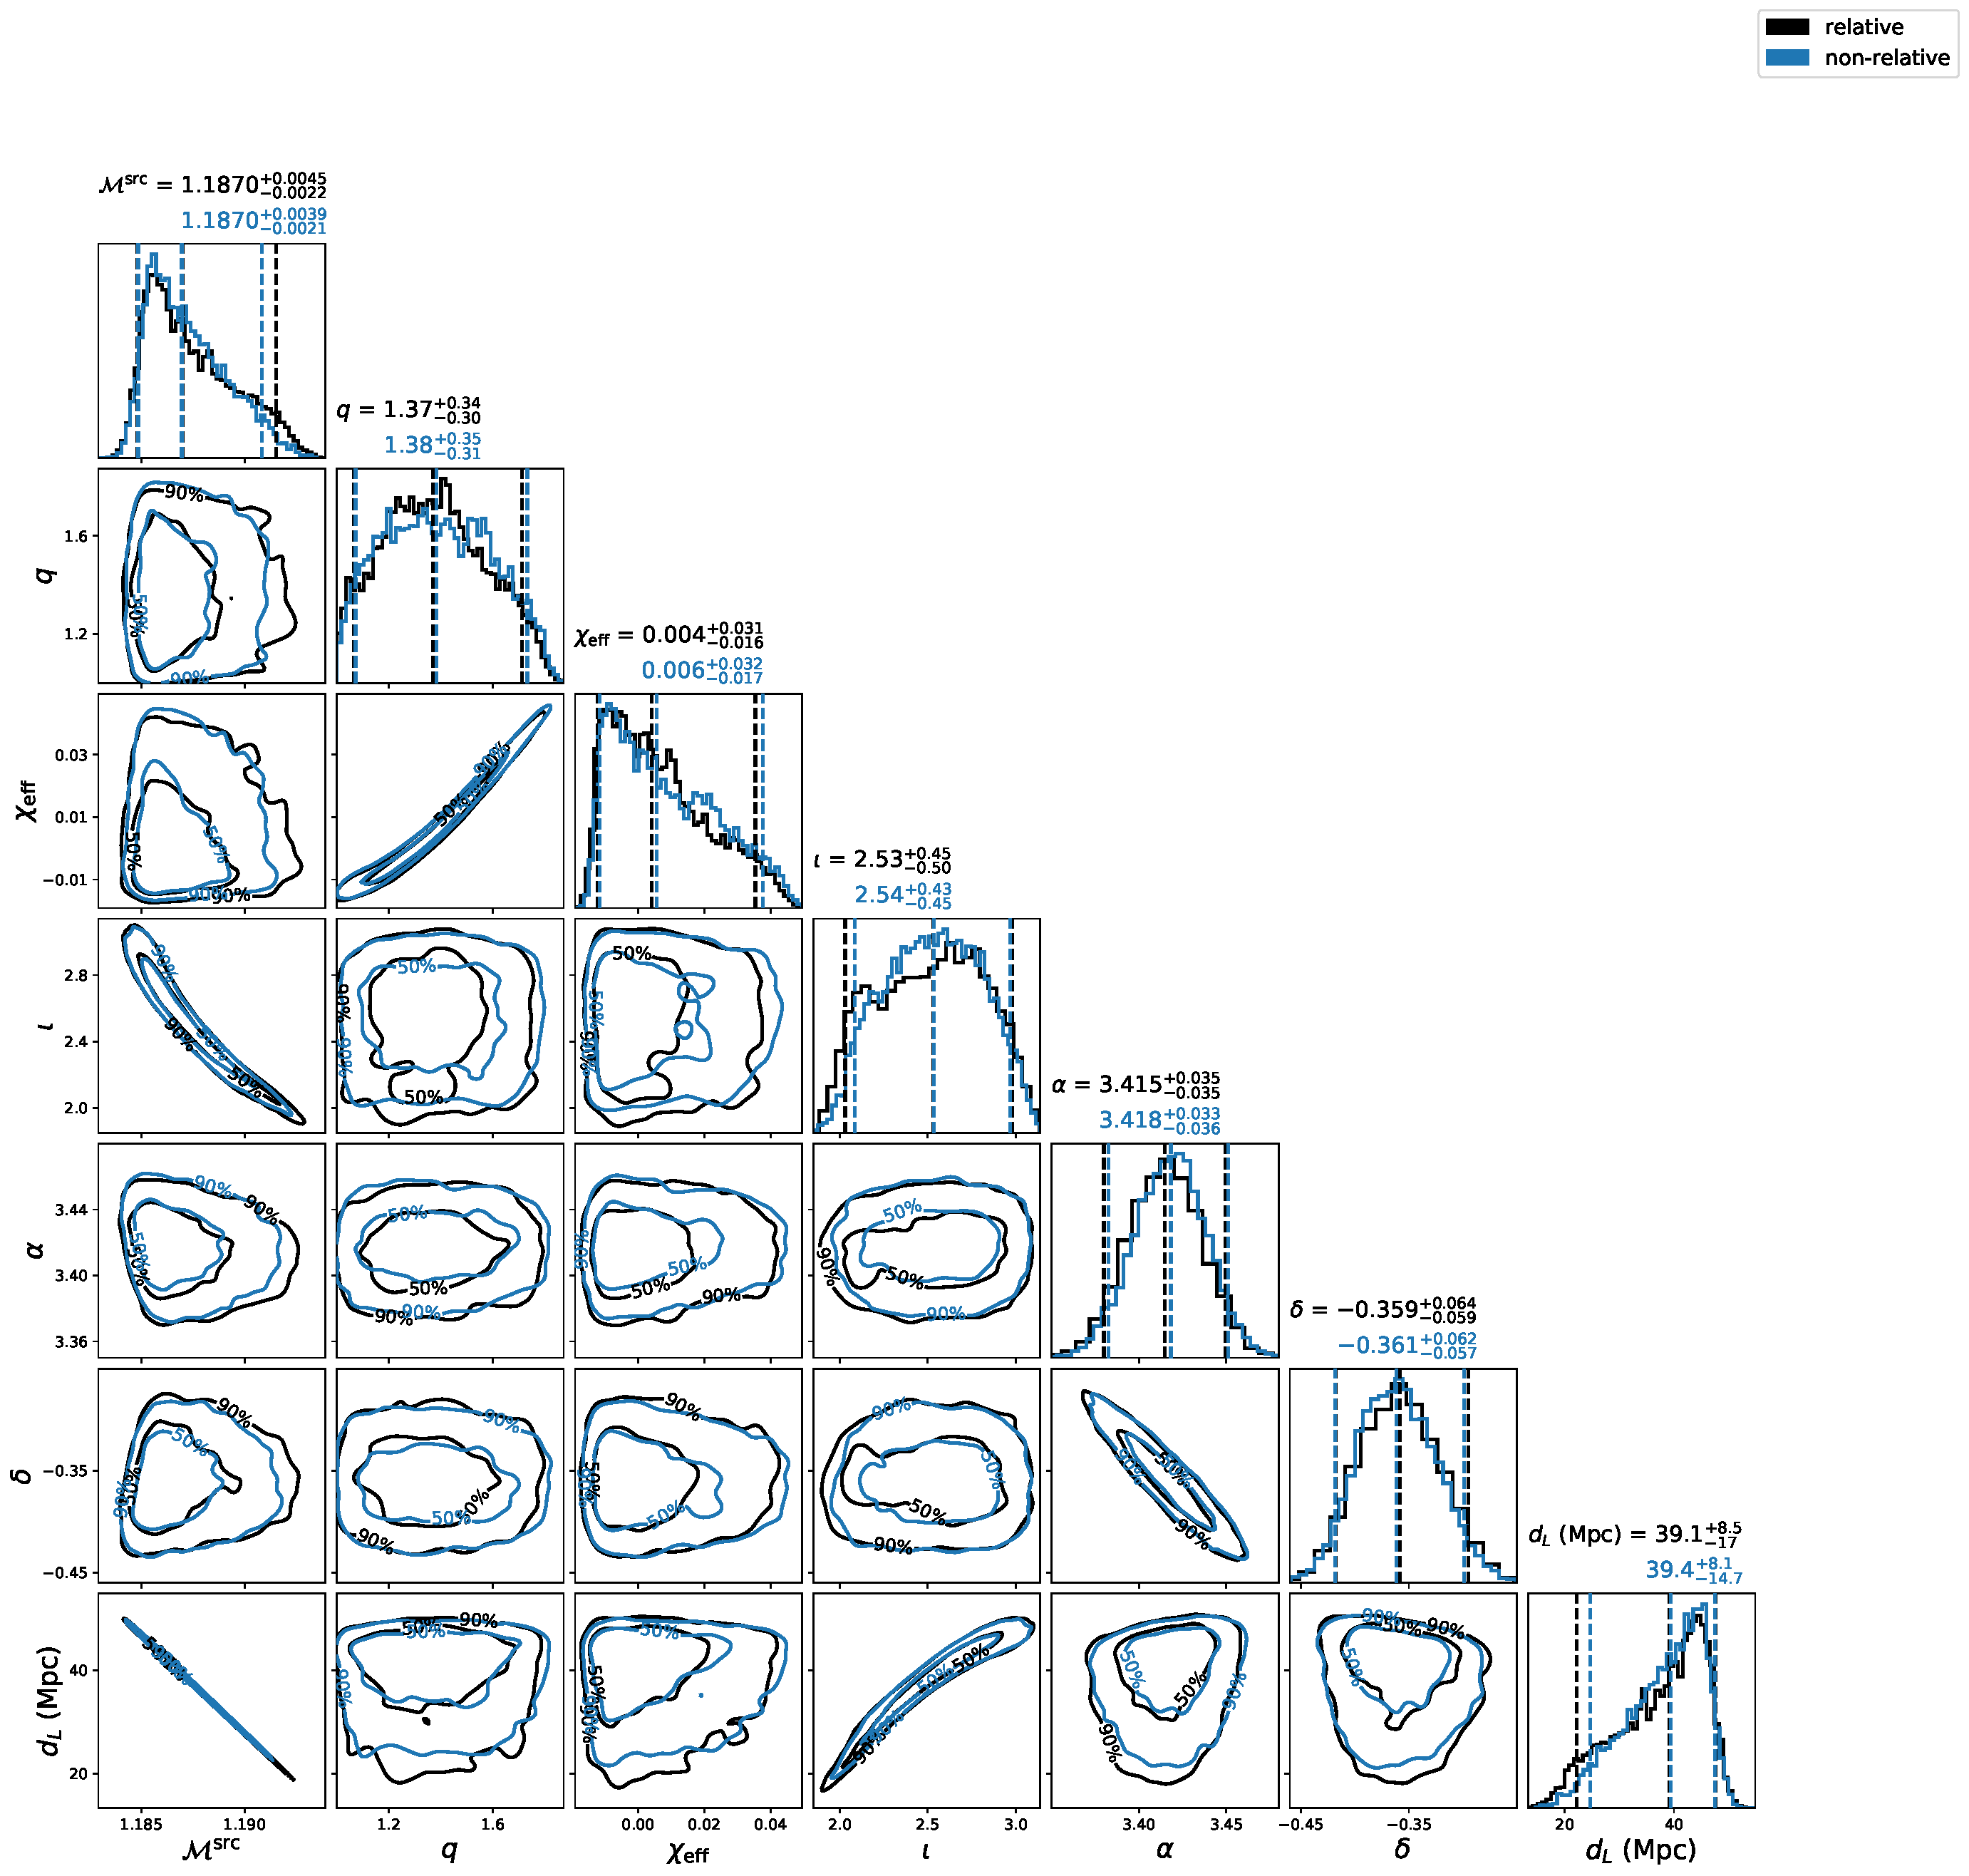
\includegraphics[width=\textwidth]{Figures/rel-bin-pe/gw170817_comparison_to_nonrel_src_frame.pdf}
\caption{Posterior distributions from a relative-binned parameter estimation analysis of GW170817 (black contour) as compared to a run using the standard non-relative likelihood (blue contour). Marginalized 1-dimensional histograms for each parameter are shown along the diagonal, with vertical dashed lines at the median value and the bounds of the 90\% credible interval. Off-diagonal plots show 2-dimensional slices of the parameter space with contours delineating the 50\% and 90\% credible regions. The relative-binned analysis completed in 20 minutes versus roughly 3 hours in the non-relative case, and all parameter distributions are consistent between the two analyses.}
\label{fig:gw170817_comparison}
\end{figure}

\section{Conclusion}\label{sec:rel_bin_conclusion}

In previous LIGO-Virgo observing runs, the information provided in low-latency to astronomers consisted of the time of the signal, an estimate of its statistical significance (false alarm rate), and a three-dimensional localization probability in sky location and distance. In the recent third observing run, two additional classifications were released that bin events into one of five broad categories (binary neutron star, binary black hole, neutron star--black hole, mass gap, or terrestrial noise) and estimate the probability that the event produced an electromagnetic counterpart \cite{Kapadia:2019uut,canton2020realtime}. Both of these methods are based on the parameters of the best-fit matched filter template recorded by the low-latency search. \cite{Biscoveanu_2019} performed a template-bank simulation that estimated that the low-latency chirp mass point estimate for binary neutron stars is accurate to $\sim 10^{-3}~\msun$, however they note that there can be significant bias in mass ratio and effective spin from the best-fit template. \cite{canton2020realtime} demonstrated that the best-fit chirp mass from a search can be used to inform a classification scheme in which the classifications are correct in a large majority of cases.

Here, we have extended the relative binning algorithm \cite{cornish2013fast,Zackay:2018qdy} for fast likelihood evaluation in gravitational-wave parameter estimation to a fully coherent detector network and demonstrated that it can be seeded by the output of a matched-filter search. We have applied our method to a set of 559 simulated signals (306 binary neutron star and 253 neutron star--black hole binaries) as well as to GW170817. We find that in all cases our method produces unbiased estimates for all measured parameters in less than 20 minutes. We have shown that our method is capable of producing full posterior distributions for all signal parameters, which do not suffer from the biases seen when attempting to measure the mass ratio and spin from the best-fit template. In the  case of GW170817, the relative-binned analysis produces results nearly identical to those from a standard analysis using the full likelihood, emphasizing our method's utility in producing fast parameter estimates that are of particular interest for electromagnetic followup.

For gravitational-wave events in LIGO's third observing run, the average time between an initial trigger alert and the first Bayesian parameter estimation results being made available was about 10 hours (although only updated sky maps are released and not measurement of the source's parameters). We have demonstrated  our method could reduce this delay time considerably, which would allow for electromagnetic followup campaigns to be conducted more efficiently.   We encourage the LIGO Scientific and Virgo collaborations to adopt these methods to provide the observing community with fast and accurate estimates of the parameters of detected signals so that these can be used to inform and prioritize electromagnetic followup strategies. Finally, we note that given the computational cost, very few large scale injection studies of low-mass gravitational-wave signals have been done. Our implementation of the relative binning method into \textit{PyCBC Inference} brings these sorts of studies within reach for even modestly equipped computing facilities.



\Chapter{Tidal Deformabilities and Radii of Neutron Stars from the Observation of GW170817}
\label{ch:common-radius}
We use gravitational-wave observations of the binary neutron star merger GW170817 to explore the tidal deformabilities and radii of neutron stars. We perform Bayesian parameter estimation with the source location and distance informed by electromagnetic observations. We also assume that the two stars have the same equation of state; we demonstrate that for stars with masses comparable to the component masses of GW170817, this is effectively implemented by assuming that the stars' dimensionless tidal deformabilities are determined by the binary's mass ratio $q$ by $\Lambda_1/\Lambda_2 = q^6$. We investigate different choices of prior on the component masses of the neutron stars. We find that the tidal deformability and 90\% credible interval is $\tilde{\Lambda}=222^{+420}_{-138}$ for a uniform component mass prior, $\tilde{\Lambda}=245^{+453}_{-151}$ for a component mass prior informed by radio observations of Galactic double neutron stars, and $\tilde{\Lambda}=233^{+448}_{-144}$ for a component mass prior informed by radio pulsars. We find a robust measurement of the common areal radius of the neutron stars across all mass priors of $8.9 \le \hat{R} \le 13.2$~km, with a mean value of $\langle \hat{R} \rangle = 10.8$~km. Our results are the first measurement of tidal deformability with a physical constraint on the star's equation of state and place the first lower bounds on the deformability and areal radii of neutron stars using gravitational waves.

\section{Introduction}
On August 17, 2017 LIGO and Virgo observed gravitational waves from a binary neutron star coalescence, GW170817~\cite{TheLIGOScientific:2017qsa}.
This observation can be used to explore the equation of state (EOS) of matter at super-nuclear densities~\cite{thorne.k:1987,Read:2009yp}. This information is encoded as a change in gravitational-wave phase evolution caused by the tidal deformation of the  neutron stars~\cite{Flanagan:2007ix}. 
At leading order, the tidal effects are imprinted in the gravitational-wave signal through the binary tidal deformability~\cite{Flanagan:2007ix,Hinderer:2007mb}
\begin{equation}
\tilde{\Lambda}
= \frac{16}{13}\frac{(12q+1)\Lambda_1+(12+q)q^4\Lambda_2}{(1+q)^5}, \label{eq:common_rad_lambda_t0}
\end{equation}
where $q = m_2/m_1 \leq 1$ is the binary's mass ratio [cf. Eq.~(34) of Ref.~\cite{Gralla:2017djj}]. The deformability of each star is
\begin{equation}
\Lambda_{1,2}=\frac{2}{3}k_2\left(\frac{R_{1,2}c^2}{Gm_{1,2}}\right)^5, \label{eq:lambda_12}
\end{equation}
where $k_2$ is the tidal Love number~\cite{Flanagan:2007ix,Hinderer:2007mb}, which depends on the star's mass and the EOS. $R_{1,2}$ and $m_{1,2}$ are the areal radii and masses of the neutron stars, respectively. 

In the results of Ref.~\cite{TheLIGOScientific:2017qsa},
the priors on $\Lambda_{1,2}$ are taken to be completely uncorrelated,
which is equivalent to assuming that each star may have a different
EOS. Here, we reanalyze the gravitational-wave data using Bayesian
inference \cite{Biwer:2018osg,alex_nitz_2018_1208115,emcee} to measure the tidal deformability, using a
correlation between $\Lambda_1$ and $\Lambda_2$ which follows from the
assumption that both stars have the same EOS.  We repeat
our analysis without the common EOS constraint and calculate the 
Bayes factor that compares the evidences for these two models.
We also fix the sky position and
distance from electromagnetic observations~\cite{Soares-Santos:2017lru,Cantiello:2018ffy}.
We study the effect of
the prior for the component masses by performing analyses with three
different priors: the first is uniform between 1 and $2M_\odot$, the
second is informed by radio observations of double neutron star
binaries, and the third is informed by the masses of isolated pulsars~\cite{Ozel:2016oaf}.

\section{The common equation of state constraint}

To explore imposing a common EOS constraint, we employ a piecewise polytrope scheme ~\cite{Lattimer:2015nhk} to simulate thousands of equations of state.  Each EOS obeys causality, connects at low densities to the well-known EOS of neutron star crusts~\cite{Lattimer:2012nd}, is constrained by experimental and theoretical studies of the symmetry properties of matter near the nuclear saturation density, and satisfies the observational constraint for the maximum mass of a neutron star, $m_\mathrm{max}\ge2M_\odot$~\cite{Antoniadis:2013pzd}. Figure~\ref{fig:lam-mass} shows the results of Tolman-Oppenheimer-Volkoff (TOV) integrations~\cite{Oppenheimer:1939ne,Postnikov:2010yn} to determine $\Lambda$ as functions of $m$, $R$, and the EOS. Each configuration is color coded according to its
radius. In the relevant mass range, $\Lambda$ generally varies as
$m^{-6}$. For a given mass $m$, there is an inherent spread of about a factor of ten in $\Lambda$, which is correlated with $R^6$. We find that the star's tidal deformability is related to its compactness parameter 
$\beta=Gm/(Rc^2)$ by the relation $\Lambda~\simeq a\beta^{-6}$. We find that $a=0.0093\pm0.0007$ bounds this relation if $1.1M_\odot\le m\le1.6M_\odot$
(note that this is a bound, not a confidence interval). The additional power of $\beta^{-1}$ in the $\Lambda-\beta$ relation, relative to $\beta^{-5}$ in Eq.~(\ref{eq:lambda_12}), originates because the dimensionless tidal Love number, $k_2$, varies roughly as $\beta^{-1}$ for masses $\geq$
$1M_\odot$, although this is not the case for all masses~\cite{Postnikov:2010yn}. For $m\to0$ we see that $k_2\to0$ so that $k_2$ is proportional to $\beta$ with a positive power, but since neutron stars with $m < 1\,M_\odot$ are physically unrealistic, that domain is not pertinent to this Letter.

We observed that, for nearly every specific EOS, the range of stellar radii in the mass range of interest for GW170817 is typically small. As long as $m_{\rm max}\ge 2M_\odot$, the piecewise polytrope study reveals $\langle \Delta R \rangle =-0.070$ km and $\sqrt{\langle(\Delta R)^2\rangle}~=0.11$ km, where $\Delta R \equiv R_{1.6}-R_{1.1}$ with $R_{1.1,1.6}$ the radii of stars with $m=1.1$ and $m=1.6M_\odot$, respectively. Therefore, for masses relevant for GW170817, each EOS assigns a common value of $\hat R$ to stellar radii with little sensitivity to the mass. We can combine the relations $\Lambda~\simeq a\beta^{-6}$ and $R_1=R_2$ to find the simple prescription $\Lambda_1=q^6\Lambda_2$. We impose the common EOS constraint in our analysis using this relation. The exponent of $q$ changes with chirp mass $\mathcal{M}$ and for $\mathcal{M} > 1.5\,M_\odot$ this relation has to be modified. However, this is not relevant for the study of GW170817.

\begin{figure}[t]
  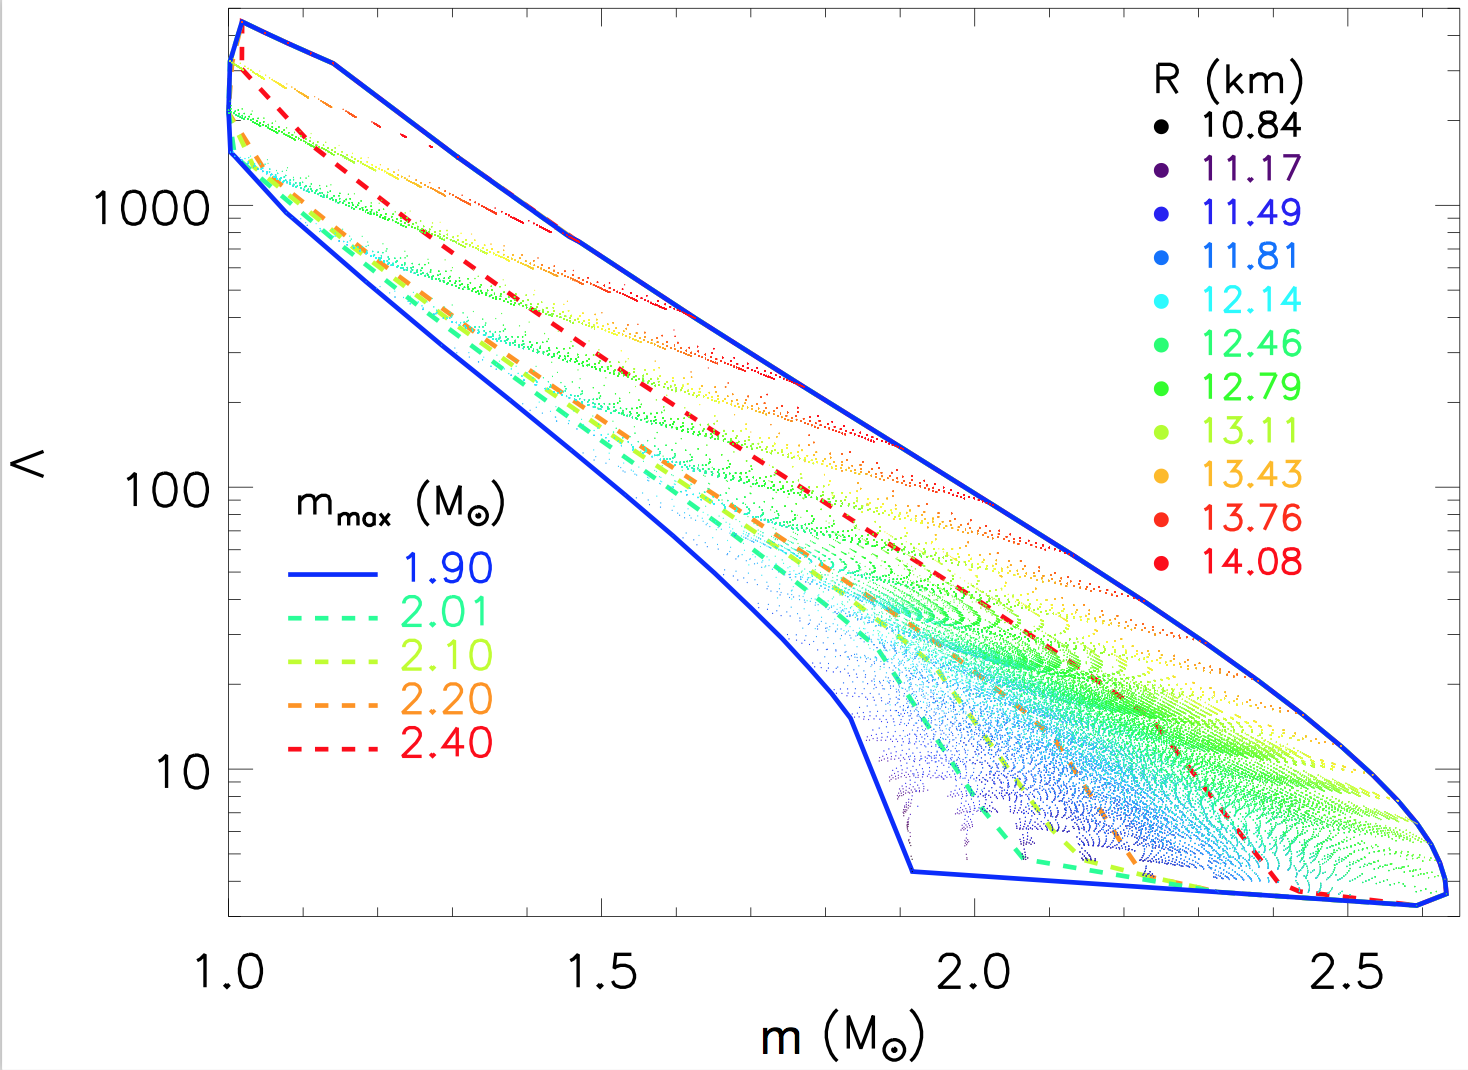
\includegraphics[width=\textwidth]{Figures/common-radius/lam-mass.png}
  \caption{The tidal deformability $\Lambda$ as a function of mass for physically realistic polytropes. A TOV integration with each EOS parameter set results in a series of values of $\Lambda(m)$ that are shown as points colored by their radii $R$. Dashed curves are lower bounds to $\Lambda$ for a given mass $m$ which vary depending on the assumed lower limit to the neutron star maximum mass, $m_\mathrm{max}$.  All values of $m_\mathrm{max}$ produce the same upper bound. \label{fig:lam-mass}}
\end{figure}



\section{Implications for the neutron star radius}

The common EOS constraint allows us to show that the binary tidal deformability $\tilde\Lambda$ is essentially a function of the chirp mass ${\cal{M}}$, the common radius $\hat R$, and the mass ratio $q$, but that its dependence on $q$ is very weak. Substituting the expressions $\Lambda~\simeq a\beta^{-6}$ and $R=\hat R$ into Eq. (\ref{eq:common_rad_lambda_t0}), we find
\begin{equation}
\tilde{\Lambda}=
\frac{16a}{13}
\left(
\frac{\hat{R}c^2}{G{\cal M}}
\right)^6 f(q).
\label{eq:lambda_t1}\end{equation}
where $f(q)$ is very weakly dependent on $q$:
\begin{equation}
f(q)=q^{8/5}(12-11q+12q^2)(1+q)^{-26/5}.
\end{equation}
For example, if we compare a binary with $q = 0.75$ to an equal mass binary, we find $f(0.75)/f(1)=1.021$. As long as $q\ge0.6$, valid for $1M_\odot\le m\le 1.6 M_\odot$ for both stars, we infer from Eq.~(\ref{eq:lambda_t1}),
\begin{equation}
\tilde{\Lambda}=a^\prime\left(\frac{\hat{R}c^2}{G{\cal M}}\right)^6,
\label{eq:lambda_t2}\end{equation}
where $a^\prime=0.0042\pm0.0004$.
%The Supplemental Material~\cite{supp} shows TOV integrations for a range of EOS that validate this relationship.
For stars with masses comparable to GW170817, the common radius $\hat R$ can be found from the inversion of Eq. (\ref{eq:lambda_t2}),
\begin{equation}
\hat R\simeq R_{1.4}\simeq (11.2\pm0.2)\frac{\cal M}{M_\odot}\left(\frac{\tilde{\Lambda}}{800}\right)^{1/6}{\rm~km}.
\label{eq:rhat}\end{equation}
The quoted errors originate from the uncertainties in $a$ and $q$, and amount, in total, to 2\%.

\section{Parameter estimation methods}

We use Bayesian inference to measure the parameters of GW170817 \cite{Christensen:2001cr}. We calculate the posterior probability density function, $p(\vec{\theta}|\vec{d}(t),H)$, for the set of parameters $\vec{\theta}$ for the gravitational-waveform model, $H$, given the LIGO Hanford, LIGO Livingston, and Virgo data $\vec{d}(t)$~\cite{Vallisneri:2014vxa,gw170817-losc}
\begin{equation}
p(\vec{\theta}|\vec{d}(t),H) = \frac{p(\vec{\theta}|H) p(\vec{d}(t)|\vec{\theta},H)}{p(\vec{d}(t)|H)}.
\label{eq:common_rad_postpdf}
\end{equation}
The prior, $p(\vec{\theta}|H)$, is the set of assumed probability distributions for the waveform parameters. The likelihood $p(\vec{d}(t)|\vec{\theta},H)$ assumes a Gaussian model for the detector noise~\cite{Rover:2006bb}. Marginalization of the likelihood to obtain the posterior probabilities is performed using Markov Chain Monte Carlo (MCMC) techniques using the \textit{PyCBC Inference} software \cite{Biwer:2018osg,alex_nitz_2018_1208115} and the parallel-tempered \textit{emcee} sampler \cite{emcee,vousden:2016,mcmc}. We fix the sky location and distance to GW170817~\cite{Soares-Santos:2017lru,Cantiello:2018ffy} and calculate the posterior probabilities for the remaining source parameters. Following Ref.~\cite{TheLIGOScientific:2017qsa}, the waveform model $H$ is the restricted TaylorF2 post-Newtonian aligned-spin model \cite{Sathyaprakash:1991mt,Buonanno:2009zt,Arun:2008kb,Mikoczi:2005dn,Bohe:2013cla,Vines:2011ud}.
%Technical details of our parameter estimation and a comparison to Fig.~5 of Ref~\cite{TheLIGOScientific:2017qsa} are provided as Supplemental Material~\cite{supp}.

To implement the common EOS constraint we construct the priors on $\Lambda_{1,2}$ according to
\begin{equation}
\Lambda_1=q^3\Lambda_s,\qquad\Lambda_2=q^{-3}\Lambda_s,
\label{eq:lambdas}\end{equation}
where $\Lambda_s \sim U[0,5000]$. We discard draws with 
$\tilde{\Lambda} > 5000$, since these values are beyond the range of all plausible EOS. The resulting prior on $\tilde\Lambda$ is uniform between $0$ and $5000$.  We also perform analyses that do not assume the common EOS constraint where we allow completely uncorrelated priors for $\Lambda_{1,2}$. This allows us to compare the evidences between these hypotheses. For the uncorrelated $\Lambda_{1,2}$ analyses, the prior for $\Lambda_1 \sim U[0,1000]$ and $\Lambda_2 \sim U[0,5000]$ with these intervals set by the range of plausible equations of state in the mass range of interest, our convention of $m_1 \geq m_2$, and discarding draws with $\tilde\Lambda > 5000$.

\begin{figure*}[t]
  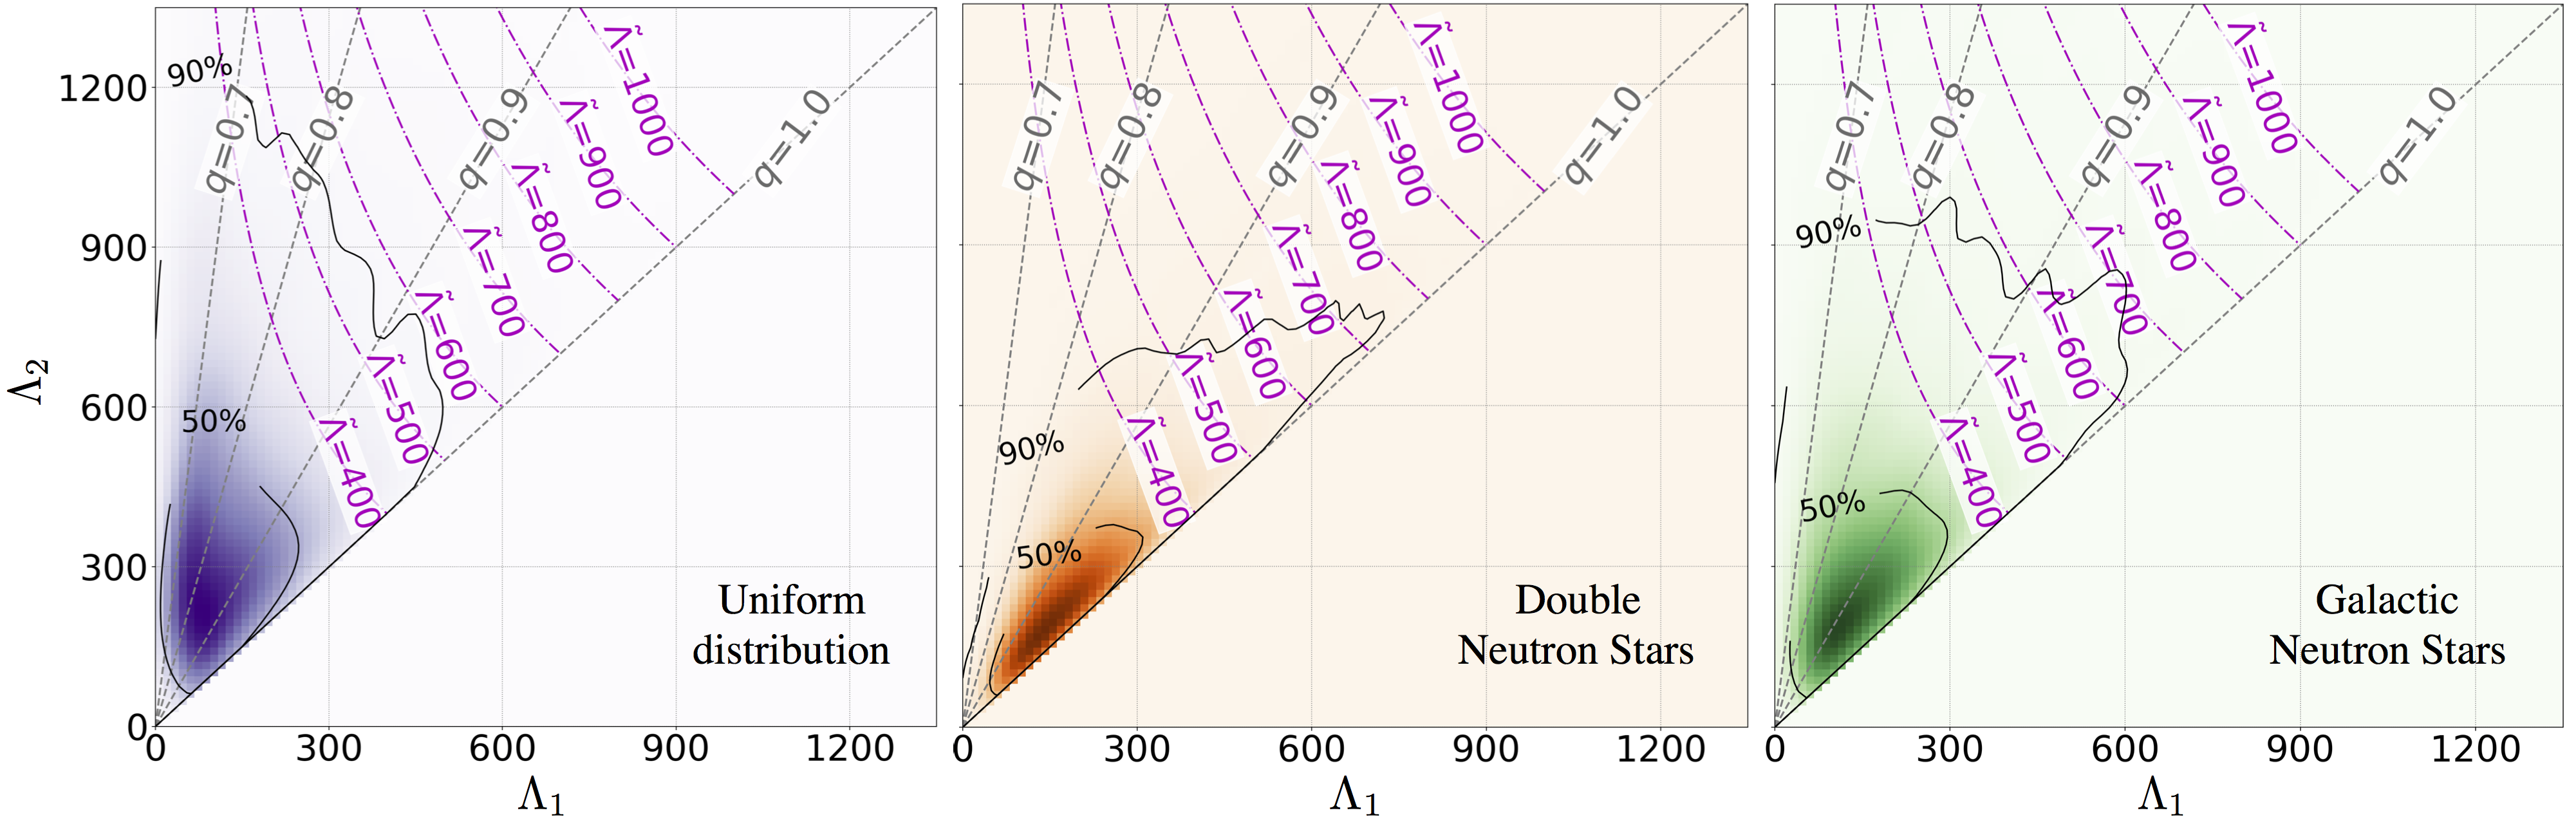
\includegraphics[width=\textwidth]{Figures/common-radius/Lambda1_2_contours_no1D_w_q_moreiter.png}
  \caption{Posterior probability densities for $\Lambda_{1,2}$ with the common EOS constraint using uniform (left), double neutron stars (middle), and Galactic neutron stars (right) component mass priors. The 50$\%$ and 90$\%$ credible region contours are shown as solid curves. Overlaid are contours of $\tilde{\Lambda}$ (in magenta) and $q$ (in gray). The values of $\Lambda_1$ and $\Lambda_2$ forbidden by causality have been excluded from the posteriors.
\label{fig:lamb12_1abc}
%
%\vspace*{-0.3cm}%
}
\end{figure*}
The choice of mass prior can have an impact on the recovery of the tidal deformability~\cite{Agathos:2015uaa}. To investigate this, we carry out our parameter estimation analyses using three different priors on the binary's component masses. First, we assume a uniform prior on each star's mass, with $m_{1,2} \sim U[1,2]\, M_\odot$. Then, we assume a Gaussian prior on the component masses $m_{1,2} \sim N(\mu = 1.33, \sigma = 0.09)\, M_\odot$, which is a fit to masses of neutron stars observed in  double neutron star systems~\cite{Ozel:2016oaf}. The third prior assumes that the component masses are drawn from a fit to the observed mass distributions of recycled and slow pulsars in the Galaxy with $m_1 \sim N(\mu = 1.54, \sigma = 0.23)\, M_\odot$ and $m_2 \sim N(\mu = 1.49, \sigma = 0.19)\, M_\odot$~\cite{Ozel:2016oaf}. We impose the constraint $m_1 \geq m_2$ which leads to $\Lambda_2 \geq \Lambda_1$. For all our analyses, the prior on the component spins is $\chi_{1,2} \sim U[-0.05,0.05]$, consistent with the expected spins of field binaries when they enter the LIGO-Virgo sensitive band~\cite{Brown:2012qf}.

% Insert PE technical details here from Supp. Materials
To measure the source parameters for GW170817, we performed parameter estimation on the Advanced LIGO-Virgo data available at the LIGO Open Science Center \cite{Vallisneri:2014vxa,gw170817-losc}. 
Our analysis was performed with the \textit{PyCBC Inference} software \cite{Biwer:2018osg,alex_nitz_2018_1208115} and the parallel-tempered \textit{emcee} sampler \cite{emcee,vousden:2016} for sampling over the parameter space using Markov Chain Monte Carlo (MCMC) techniques \cite{mcmc}. 

The LOSC data files include a post-processing noise subtraction performed by the LIGO-Virgo Collaboration \cite{gw170817-losc,gw170817-noise}. The LOSC documentation states that these data have been truncated to remove tapering effects due to the cleaning process \cite{gw170817-losc}, however the LOSC data shows evidence of tapering after GPS time $1187008900$ in the LIGO Hanford detector. To avoid any contamination of our results we do not use any data after GPS time $1187008891$. The power spectral density (PSD) used to construct the likelihood was calculated using Welch's method \cite{1161901} with 16~second Hann-windowed segments (overlapped by 8~s) taken from GPS time $1187007048$ to $1187008680$. The PSD estimate is truncated to 8~s length in the time domain using the method described in Ref. \cite{Allen:2005fk}. The gravitational-wave data used in the likelihood is taken from the interval $1187008691$ to $1187008891$. 

Ref.~\cite{Abbott:2018wiz} found that choice of the low-frequency cutoff can have an effect on the measurement of the neutron star tidal deformability and used a different power spectral density estimation technique to that used in our analysis~\cite{Littenberg:2014oda}. We investigated the effect of changing our estimate of the power spectral density with the power spectral density released as supplemental materials to Ref.~\cite{Abbott:2018wiz}. We find that the change in parameter measurements is smaller than the statistical errors, and conclude that the choice of power spectral density estimation technique does not affect our results. To investigate the choice of low-frequency cutoff, we computed the measurabilities of the chirp mass $\mathcal{M}$, signal-to-noise ratio $\rho$, and binary deformability $\tilde{\Lambda}$ in the frequency range 10-2000~Hz. These are defined as the integrand as a function of frequency of the noise moment integrals $I_{\mathrm 10}$, $I_{\mathrm 0}$, and $I_{\mathrm -10}$ (see Ref.~\cite{Damour:2012yf}) and shown in Fig.~\ref{fig:measurability}. It can be seen that the signal-to-noise ratio is non-zero down to a frequency of $\sim$ 20~Hz for all the three detectors. While detector sensitivity at this frequency does not affect the measurability of $\tilde\Lambda$, it does affect the measurability of the chirp mass $\mathcal{M}$. We repeated our analyses at 25~Hz, 23~Hz, and 20~Hz, and found an improvement in the $\mathcal{M}$ measurement when extending until the low-frequency cutoff was 20~Hz. Consequently, we evaluated the likelihood from a low-frequency cutoff of 20~Hz to the Nyquist frequency of 2048~Hz. The improved measurement of $\mathcal{M}$ eliminates regions of higher $\tilde{\Lambda}$ values from the posterior probability densities, and hence better constrains the measurement of this parameter, as shown in Fig~\ref{fig:posterior_overlap}.

\begin{figure}[t]
  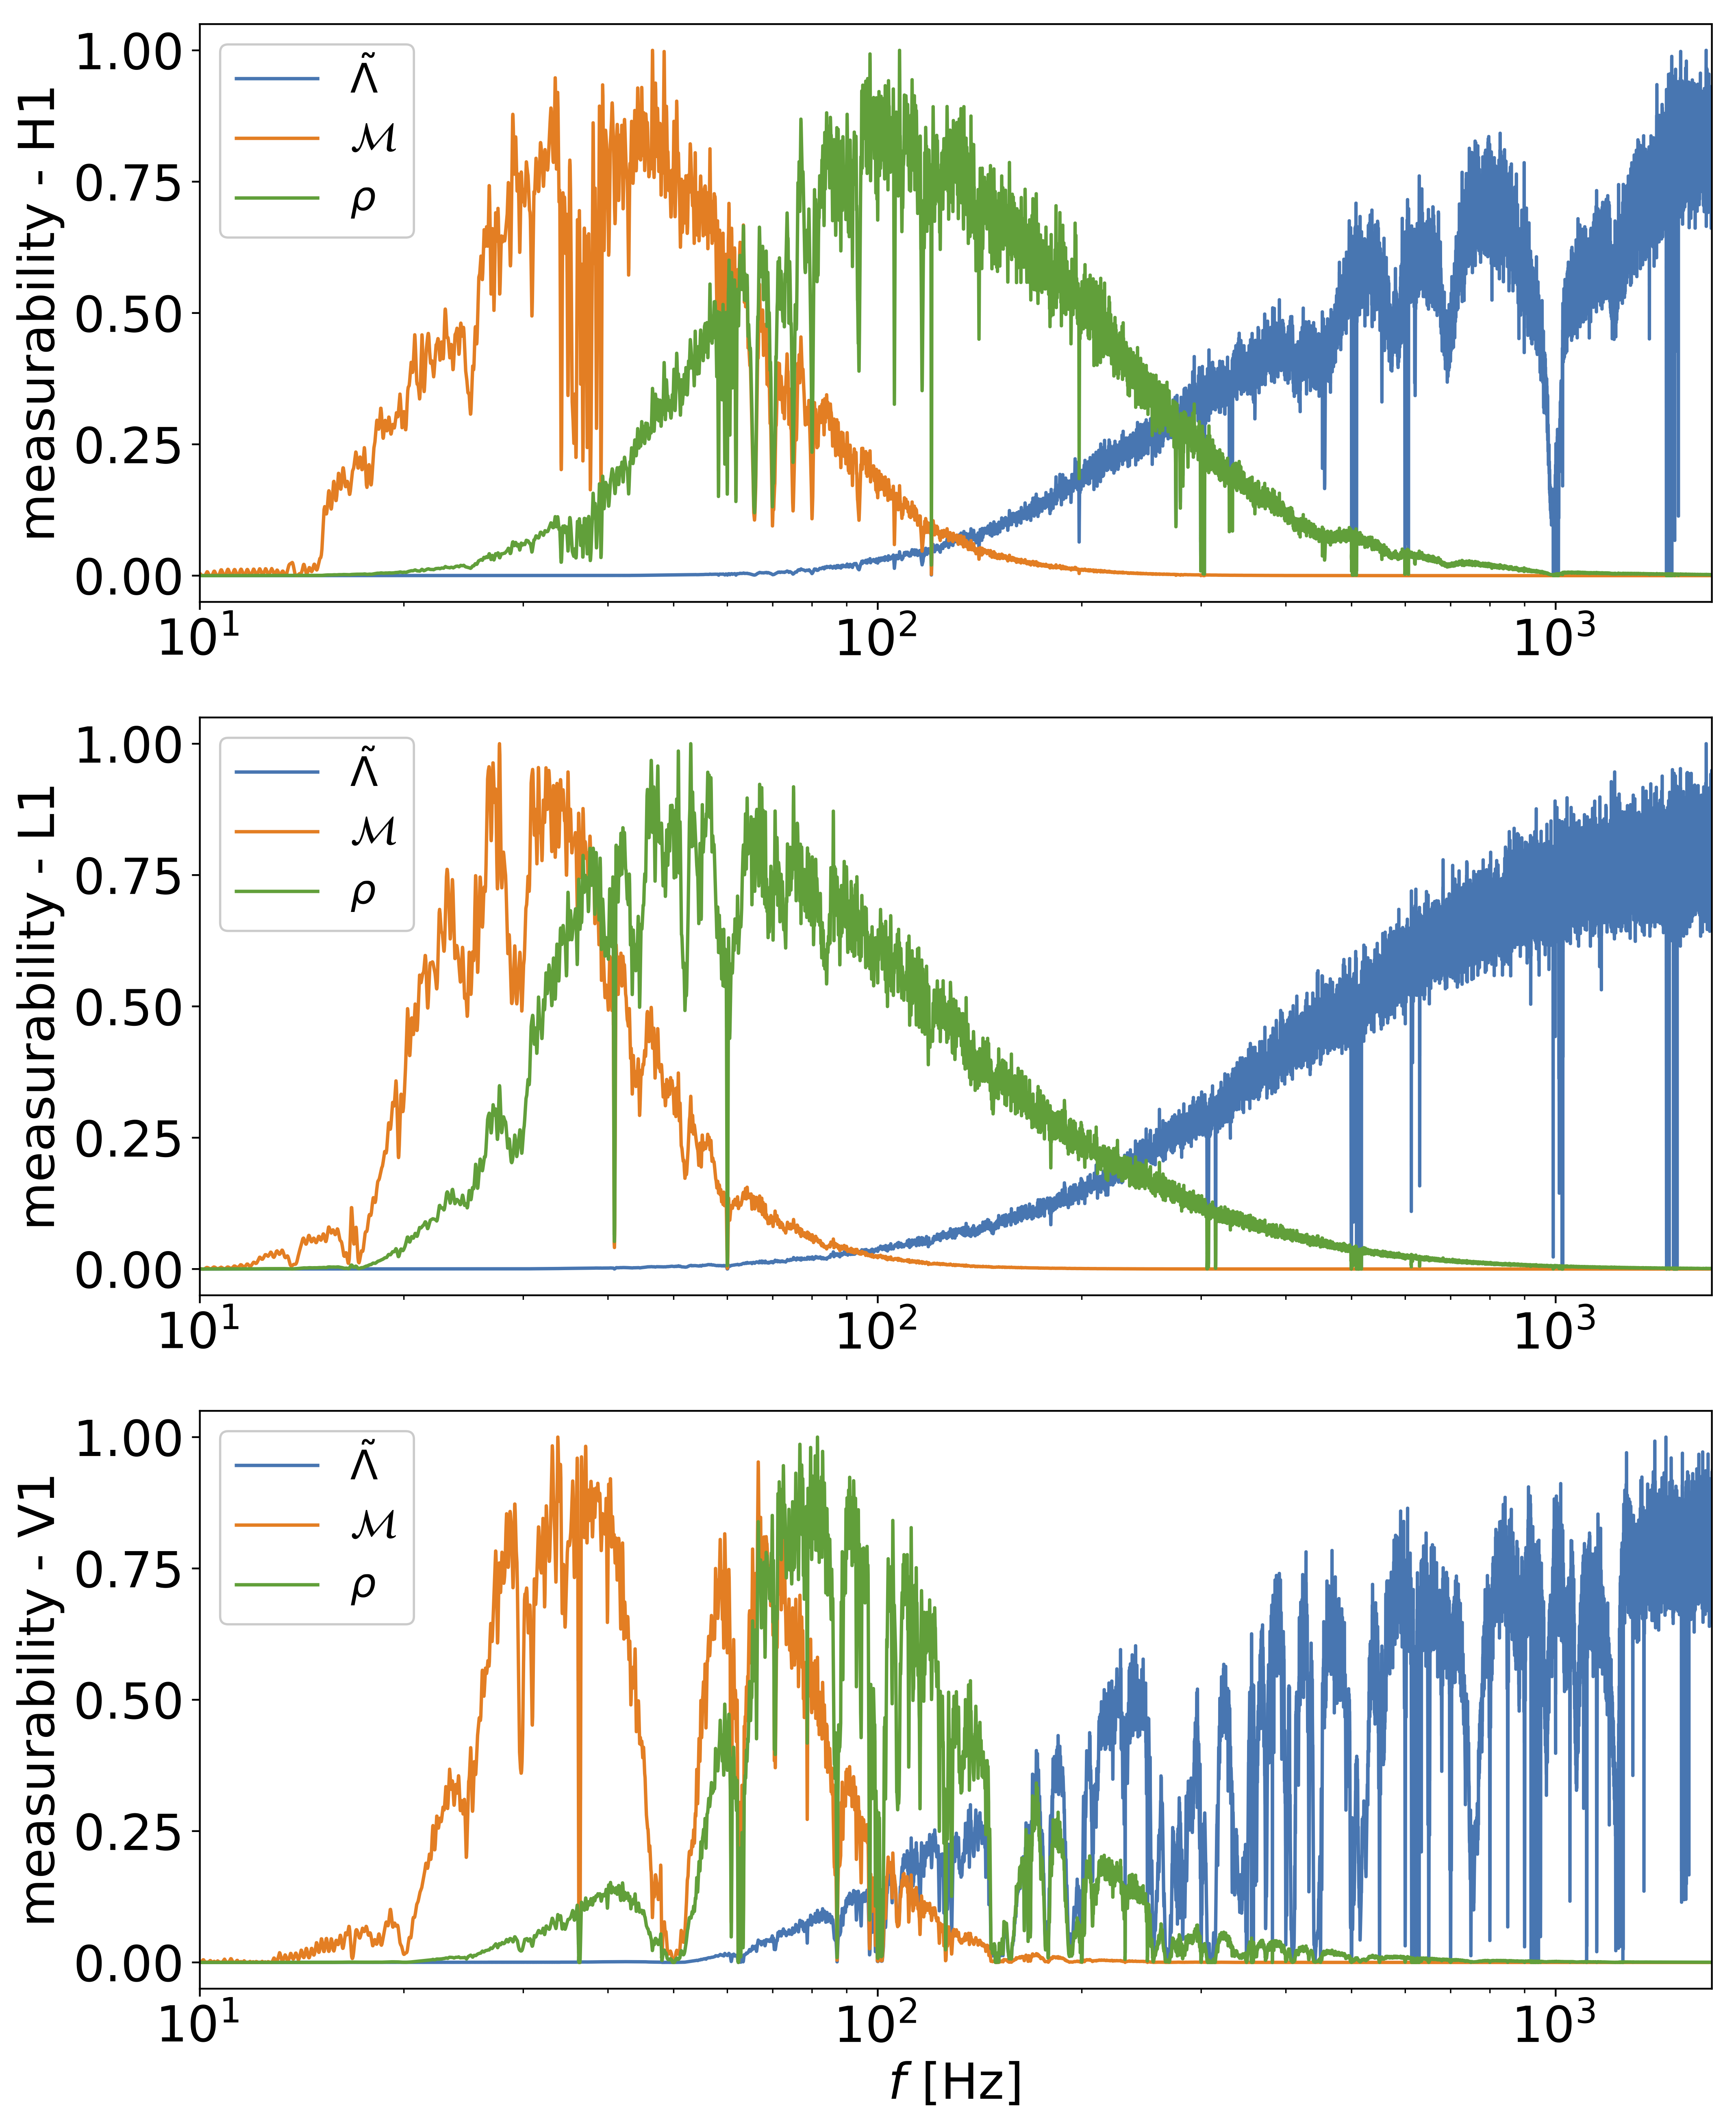
\includegraphics[width=14cm]{Figures/common-radius/measurability_plots.png}
  \caption{Measurability~\cite{Damour:2012yf} of the chirp mass $\mathcal{M}$, SNR $\rho$ and binary deformability $\tilde{\Lambda}$ in the frequency range 10 Hz - 2000 Hz. Each detector's parameter measurability is scaled to the maximum frequency to show the relative accumulation of measurement over the detector's frequency band. Note that between detectors, L1 is more sensitive than H1, which is more sensitive than V1. Measurability of chirp mass is accumulated primarily at low frequencies, whereas measurability of tidal deformability is accumulated at higher frequencies. We extend computation of the likelihood down to $20$~Hz where the measured signal-to-noise ratio (the logarthim of the likelihood) drops to zero in all three detectors. 
  \label{fig:measurability}}
\end{figure}

The templates for the waveforms used in our parameter estimation analysis are generated using the restricted TaylorF2 waveform model, a Fourier domain waveform model generated using stationary phase approximation. We use the implementation from the LIGO Algorithm Library (LAL)~\cite{lal} accurate to 3.5 post-Newtonian (pN) order in orbital phase \cite{Buonanno:2009zt}, 2.0 pN order in spin-spin, quadrupole-monopole and self-spin interactions\cite{Arun:2008kb,Mikoczi:2005dn}, and 3.5 pN order in spin-orbit interactions \cite{Bohe:2013cla}. The tidal corrections enter at the 5 pN and 6 pN orders~\cite{Vines:2011ud}. The waveforms are terminated at twice the orbital frequency of a test particle at the innermost stable circular orbit of a Schwarzschild black hole of mass $M = m_1 + m_2$, where $m_{1,2}$ are the masses of the binary's component stars. The TaylorF2 model assumes that the spins of the neutron stars are aligned with the orbital angular momentum. Binary neutron stars formed in the field are expected to have small spins, and precession of the binary's orbital plane is not significant~\cite{Brown:2012qf}. 

We fix the sky location of the binary to the right ascension RA =  $197.450374^\circ$ and declination Dec = $-23.381495^\circ$ \cite{Soares-Santos:2017lru} for all of our runs. We also fix the luminosity distance of NGC\,4993 $d_L = 40.7$~Mpc~\cite{Cantiello:2018ffy}. The small error in the known distance of NGC\,4993 produces errors that are much smaller than the errors in measuring the tidal deformability. We have checked that including the uncertainty in the distance error does not affect our conclusions of the tidal deformabilities or radius. The MCMC computes the marginalized posterior probabilities for the remaining source parameters: chirp mass $\mathcal{M}$, mass ratio $q$, the component (aligned) spins $\chi_{1,2} = c J_{1,2}/G m_{1,2}^2$, component tidal deformabilities $\Lambda_{1,2}$, polarization angle $\psi$, inclination angle $\iota$, coalescence phase $\phi_c$, and coalescence time $t_c$. When generating the waveform in the MCMC, each $m_{1, 2}$ draw follows the constraint $m_1 \geq m_2$, and the masses are transformed to the detector frame chirp mass $\mathcal{M}^\mathrm{det}$ and $q$ with a restriction $1.1876 \le \mathcal{M}^\mathrm{det} \le 1.2076$.

\begin{figure}[b]
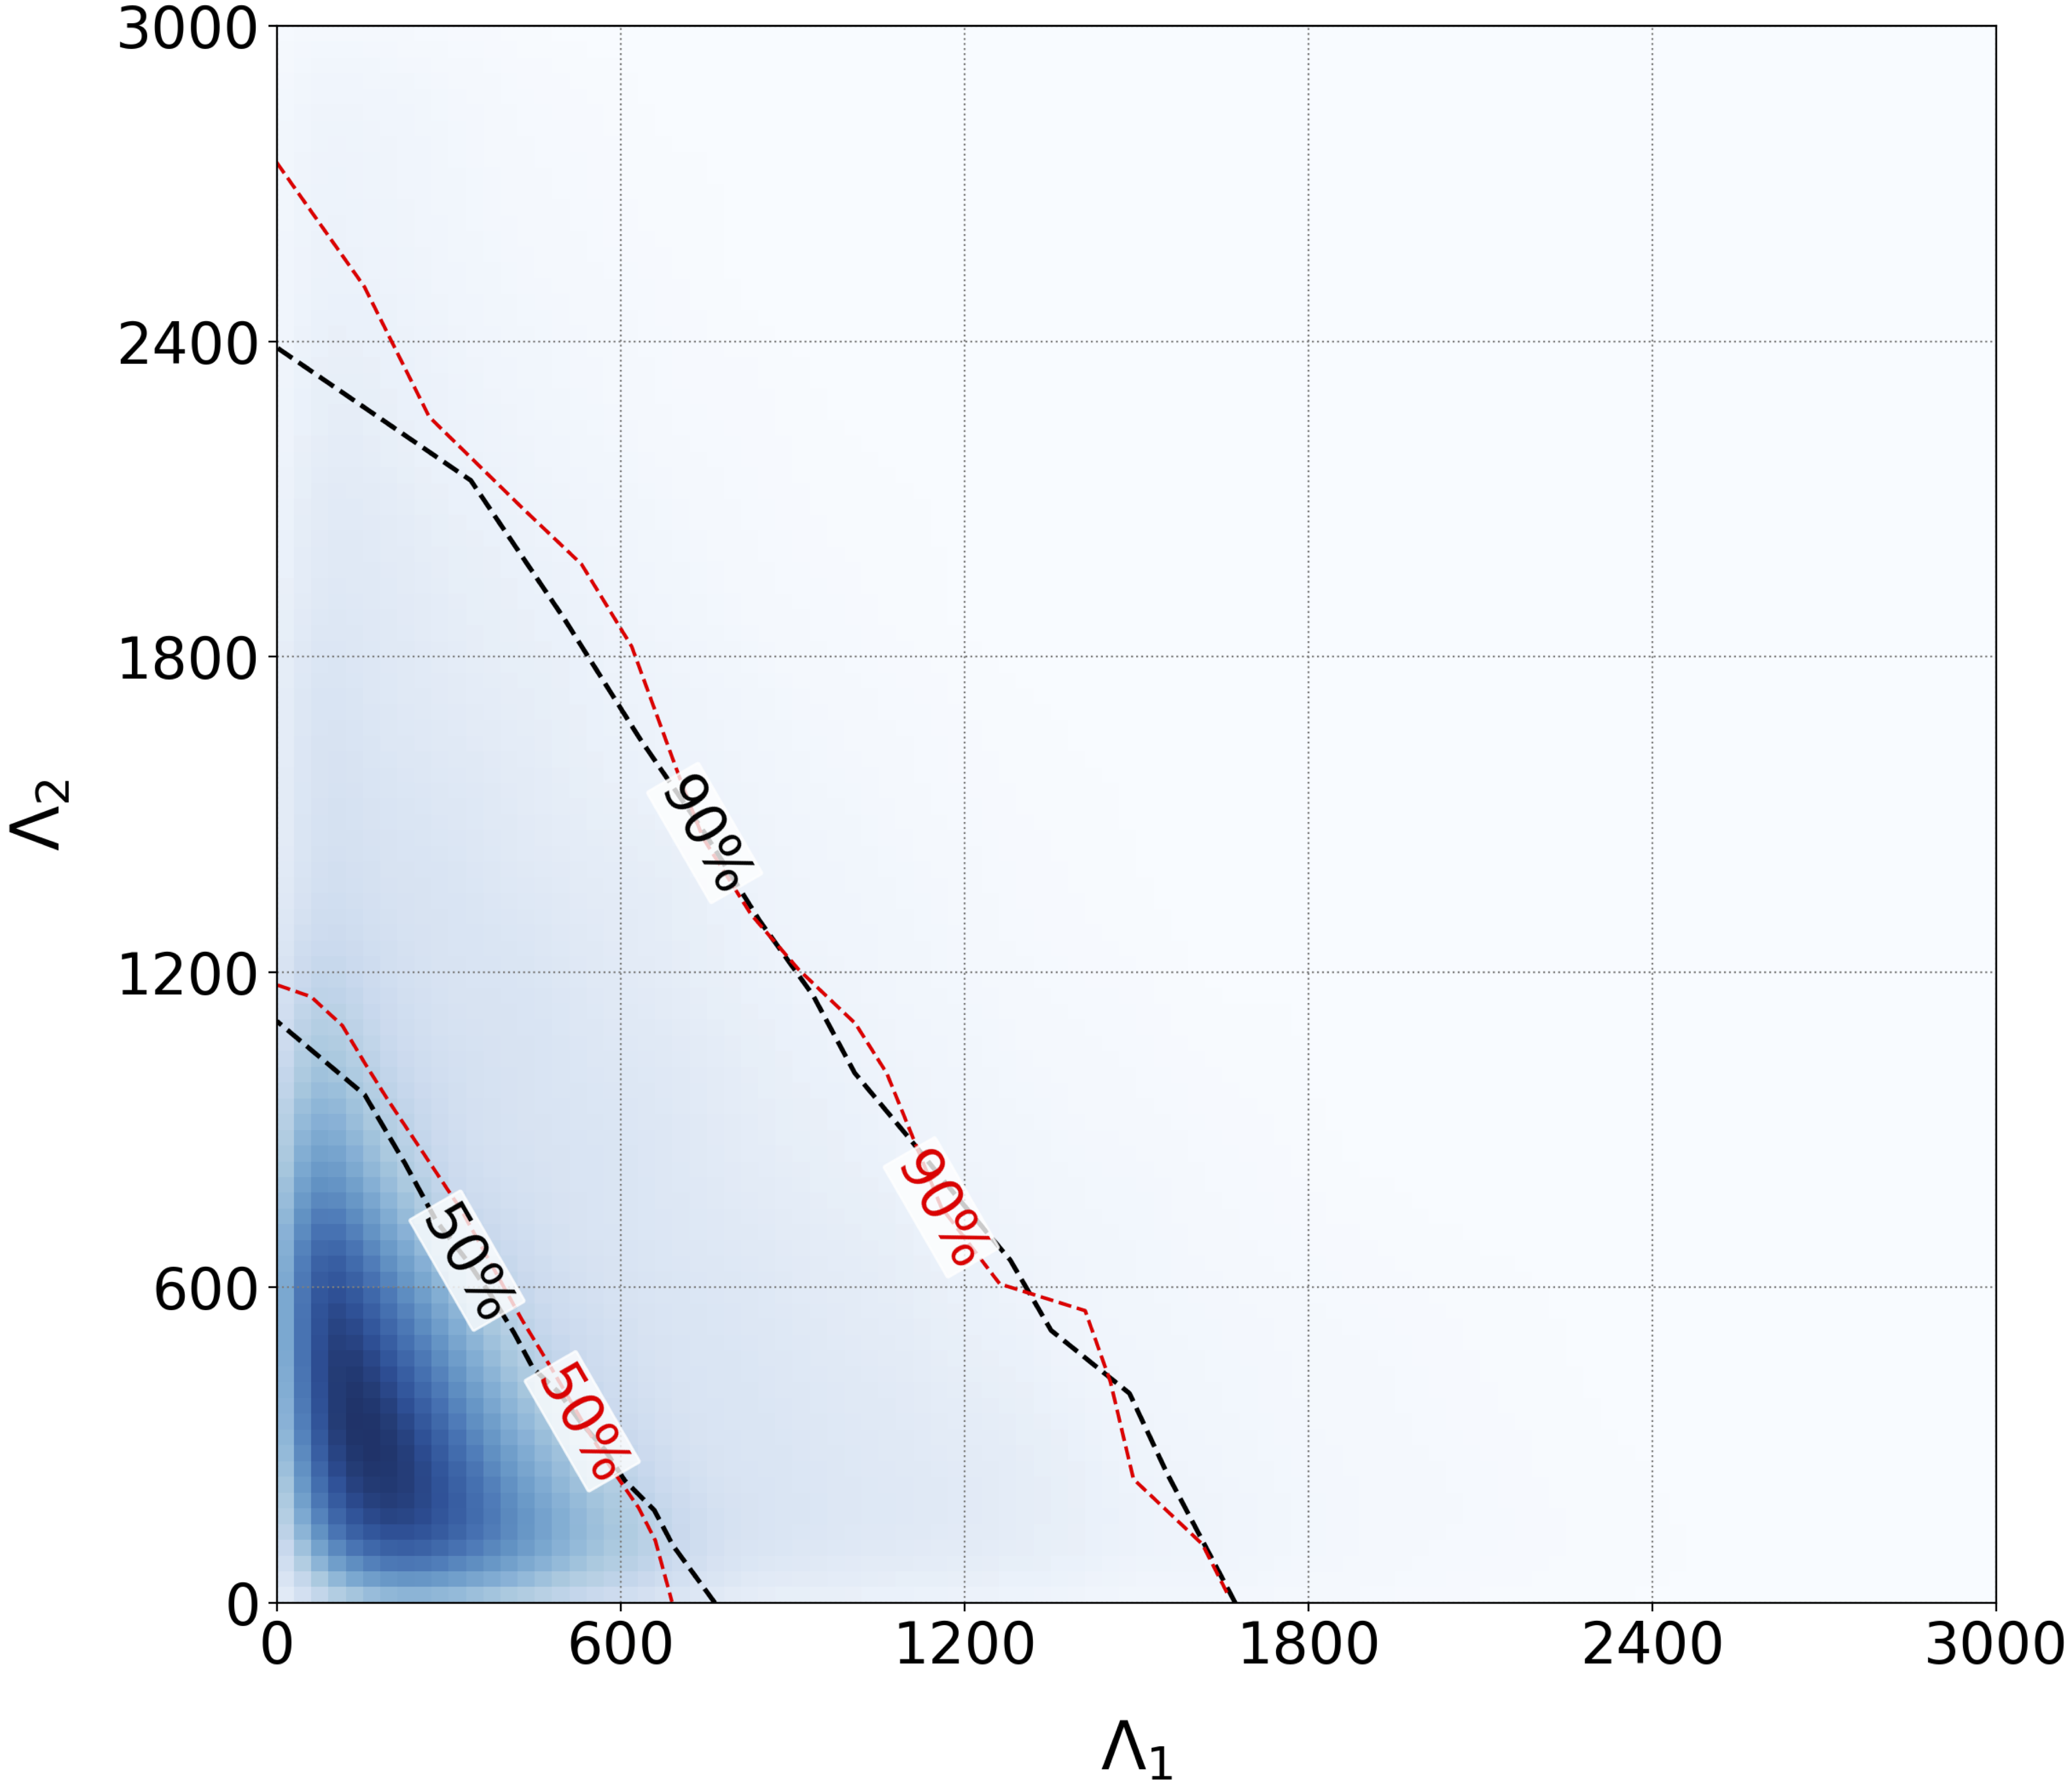
\includegraphics[width=\textwidth]{Figures/common-radius/lambda1_2_3x_ul.png}
\caption{Posterior probability density function for $\Lambda_1$, $\Lambda_2$ from unconstrained $\Lambda_{1,2} \sim U[0, 3000]$, $m_{1,2} \sim U[1, 2]$ M$_\odot$, $1.1876 \leq \mathcal{M} \leq 1.2076$, $m_1 \geq m_2$, 30~Hz low-frequency cutoff analysis. The black dotted lines show 50\% and 90\% upper limits from our analysis. The red dotted lines show 50\% and 90\% upper limits from the LIGO-Virgo analysis \cite{TheLIGOScientific:2017qsa}. } 
\label{fig:lv_compare}
\end{figure}

For direct comparison with the results of Ref.~\cite{TheLIGOScientific:2017qsa}, Fig~\ref{fig:lv_compare} shows the posterior probability densities for $\Lambda_{1,2}$ for an MCMC using a $30$~Hz low-frequency cutoff for the uniform component mass prior $m_{1,2} \sim U[1,2]\, M_\odot$, and assuming that the priors on $\Lambda_{1,2}$ are completely uncorrelated ($\Lambda_{1,2} \sim U[0,3000]$). No cut is placed on $\tilde\Lambda$ in this analysis. We have digitized the 50\% and 90\% contours from Fig.~5 of Ref.~\cite{TheLIGOScientific:2017qsa} and compared them to 50\% and 90\% upper limit contours for our result computed using a radial binning to enclose 50\% and 90\% of the posterior probability starting from $\Lambda_1 = \Lambda_2 = 0$. The 90\% contours agree well, with a slight difference in the 50\% contours. Given the accuracy of measuring the tidal deformability, this difference can 
be attributed to small differences in the technical aspects of our analysis compared to that of Ref.~\cite{TheLIGOScientific:2017qsa}. We note that the 90\% confidence contour of Fig.~5 in Ref.~\cite{TheLIGOScientific:2017qsa} with $\Lambda_1=\Lambda_2$, passes through $\tilde\Lambda \approx 1100$. If we impose $\Lambda_1=q^6 \Lambda_2$, then this contour continues to follow $\tilde\Lambda \approx 1100$ for $q \leq 1$. We interpret the difference between this result and the result of Table~I of Ref.~\cite{TheLIGOScientific:2017qsa} $\tilde\Lambda \le 800$ (90\% confidence) as being due to a different choice of prior on $\tilde\Lambda$ (one non-uniform and one uniform).

\begin{figure}[t]
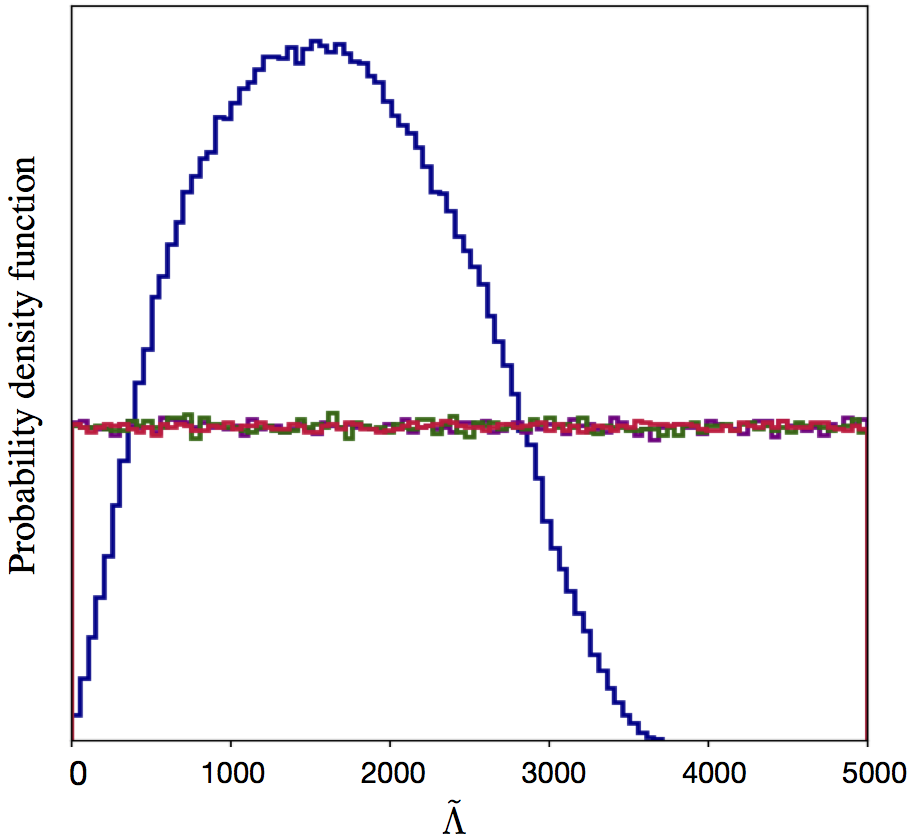
\includegraphics[width=\textwidth]{Figures/common-radius/prior_lambdatilde.png}
\caption{Comparison of the prior probability distributions on $\tilde\Lambda$ for the three mass priors imposing the common EOS constraint: uniform (purple), double neutron stars (red), galactic neutron stars (green) with a prior in $\Lambda_{1,2} \sim U[0, 3000]$ and $m_{1,2} \sim U[1, 2] M_\odot$, $m_1 \geq m_2$ without the common EOS constraint (blue). The priors in the common EOS analysis are uniform across the region of interest.} 
\label{fig:lambda_priors}
\end{figure}


Our common equation of state constraint is implemented in the MCMC by drawing a variable $\Lambda_s \sim U[0,5000]$, drawing the component masses from their respective priors and computing
\begin{equation}
\Lambda_1=q^3\Lambda_s,\qquad\Lambda_2=q^{-3}\Lambda_s,
\label{eq:lambdas_supp}\end{equation}
with draws that have $\tilde\Lambda > 5000$ discarded. This produces a prior that is uniform in $\tilde\Lambda$ between 0 and 5000, as shown in Fig.~\ref{fig:lambda_priors} for all of our three mass priors discussed in the main text. For comparison, we also show the prior on $\tilde\Lambda$ computed assuming independent $\Lambda_{1,2} \sim U[0,3000]$ and the component mass prior $m_{1,2}\sim U[1,2]\,M_\odot$. It can be seen that this prior vanishes as $\tilde\Lambda \rightarrow 0$ and so can bias the posterior at low values of   $\tilde\Lambda$. In addition to the physical requirement of a common EOS constraint, the prior used in the common EOS analysis is uniform as $\tilde\Lambda \rightarrow 0$, allowing us to fully explore likelihoods in this region, and set lower bounds on our credible intervals.

\section{Results}

%We perform parameter estimation for each mass prior with and without the common EOS constraint and calculate the Bayes factor---the ratio of the evidences $p(\vec{d}(t)|H)$---between the common EOS constrained and unconstrained analyses. We find Bayes factors $\mathcal{B}$ of 369, 125, and 612 for the three mass priors, respectively, indicating that the data strongly favor the common EOS constraint in all cases. 

Fig.~\ref{fig:posterior_overlap} shows the posterior probability densities for the parameters of interest in our study: the source frame chirp mass $\mathcal{M}^\mathrm{src}$; the mass ratio $q=m_2/m_1$; the source frame component masses $m_{1,2}^\mathrm{src}$ (which are functions of $\mathcal{M}^\mathrm{src}$ and $q$); the effective spin $\chi_\mathrm{eff} = (m_1 \chi_1 + m_2 \chi_2) / (m_1 + m_2)$; and the binary tidal deformability $\tilde{\Lambda}$. Posterior probability densities are shown for the uniform mass prior, double neutron star mass prior, and the Galactic neutron star mass prior analyses with 20~Hz low-frequency cutoff, and the uniform mass prior analyses with 25~Hz low-frequency cutoff. All the four analyses had the common EOS constraint and the causal $\Lambda(m)$ lower limit imposed. Electronic files containing the thinned posterior probability densities and an IPython notebook \cite{PER-GRA:2007} for manipulating these data are available at Ref.~\cite{gw170817commoneos}.


\begin{figure}
\begin{adjustwidth}{-1.5cm}{-0.8cm}
\centering
  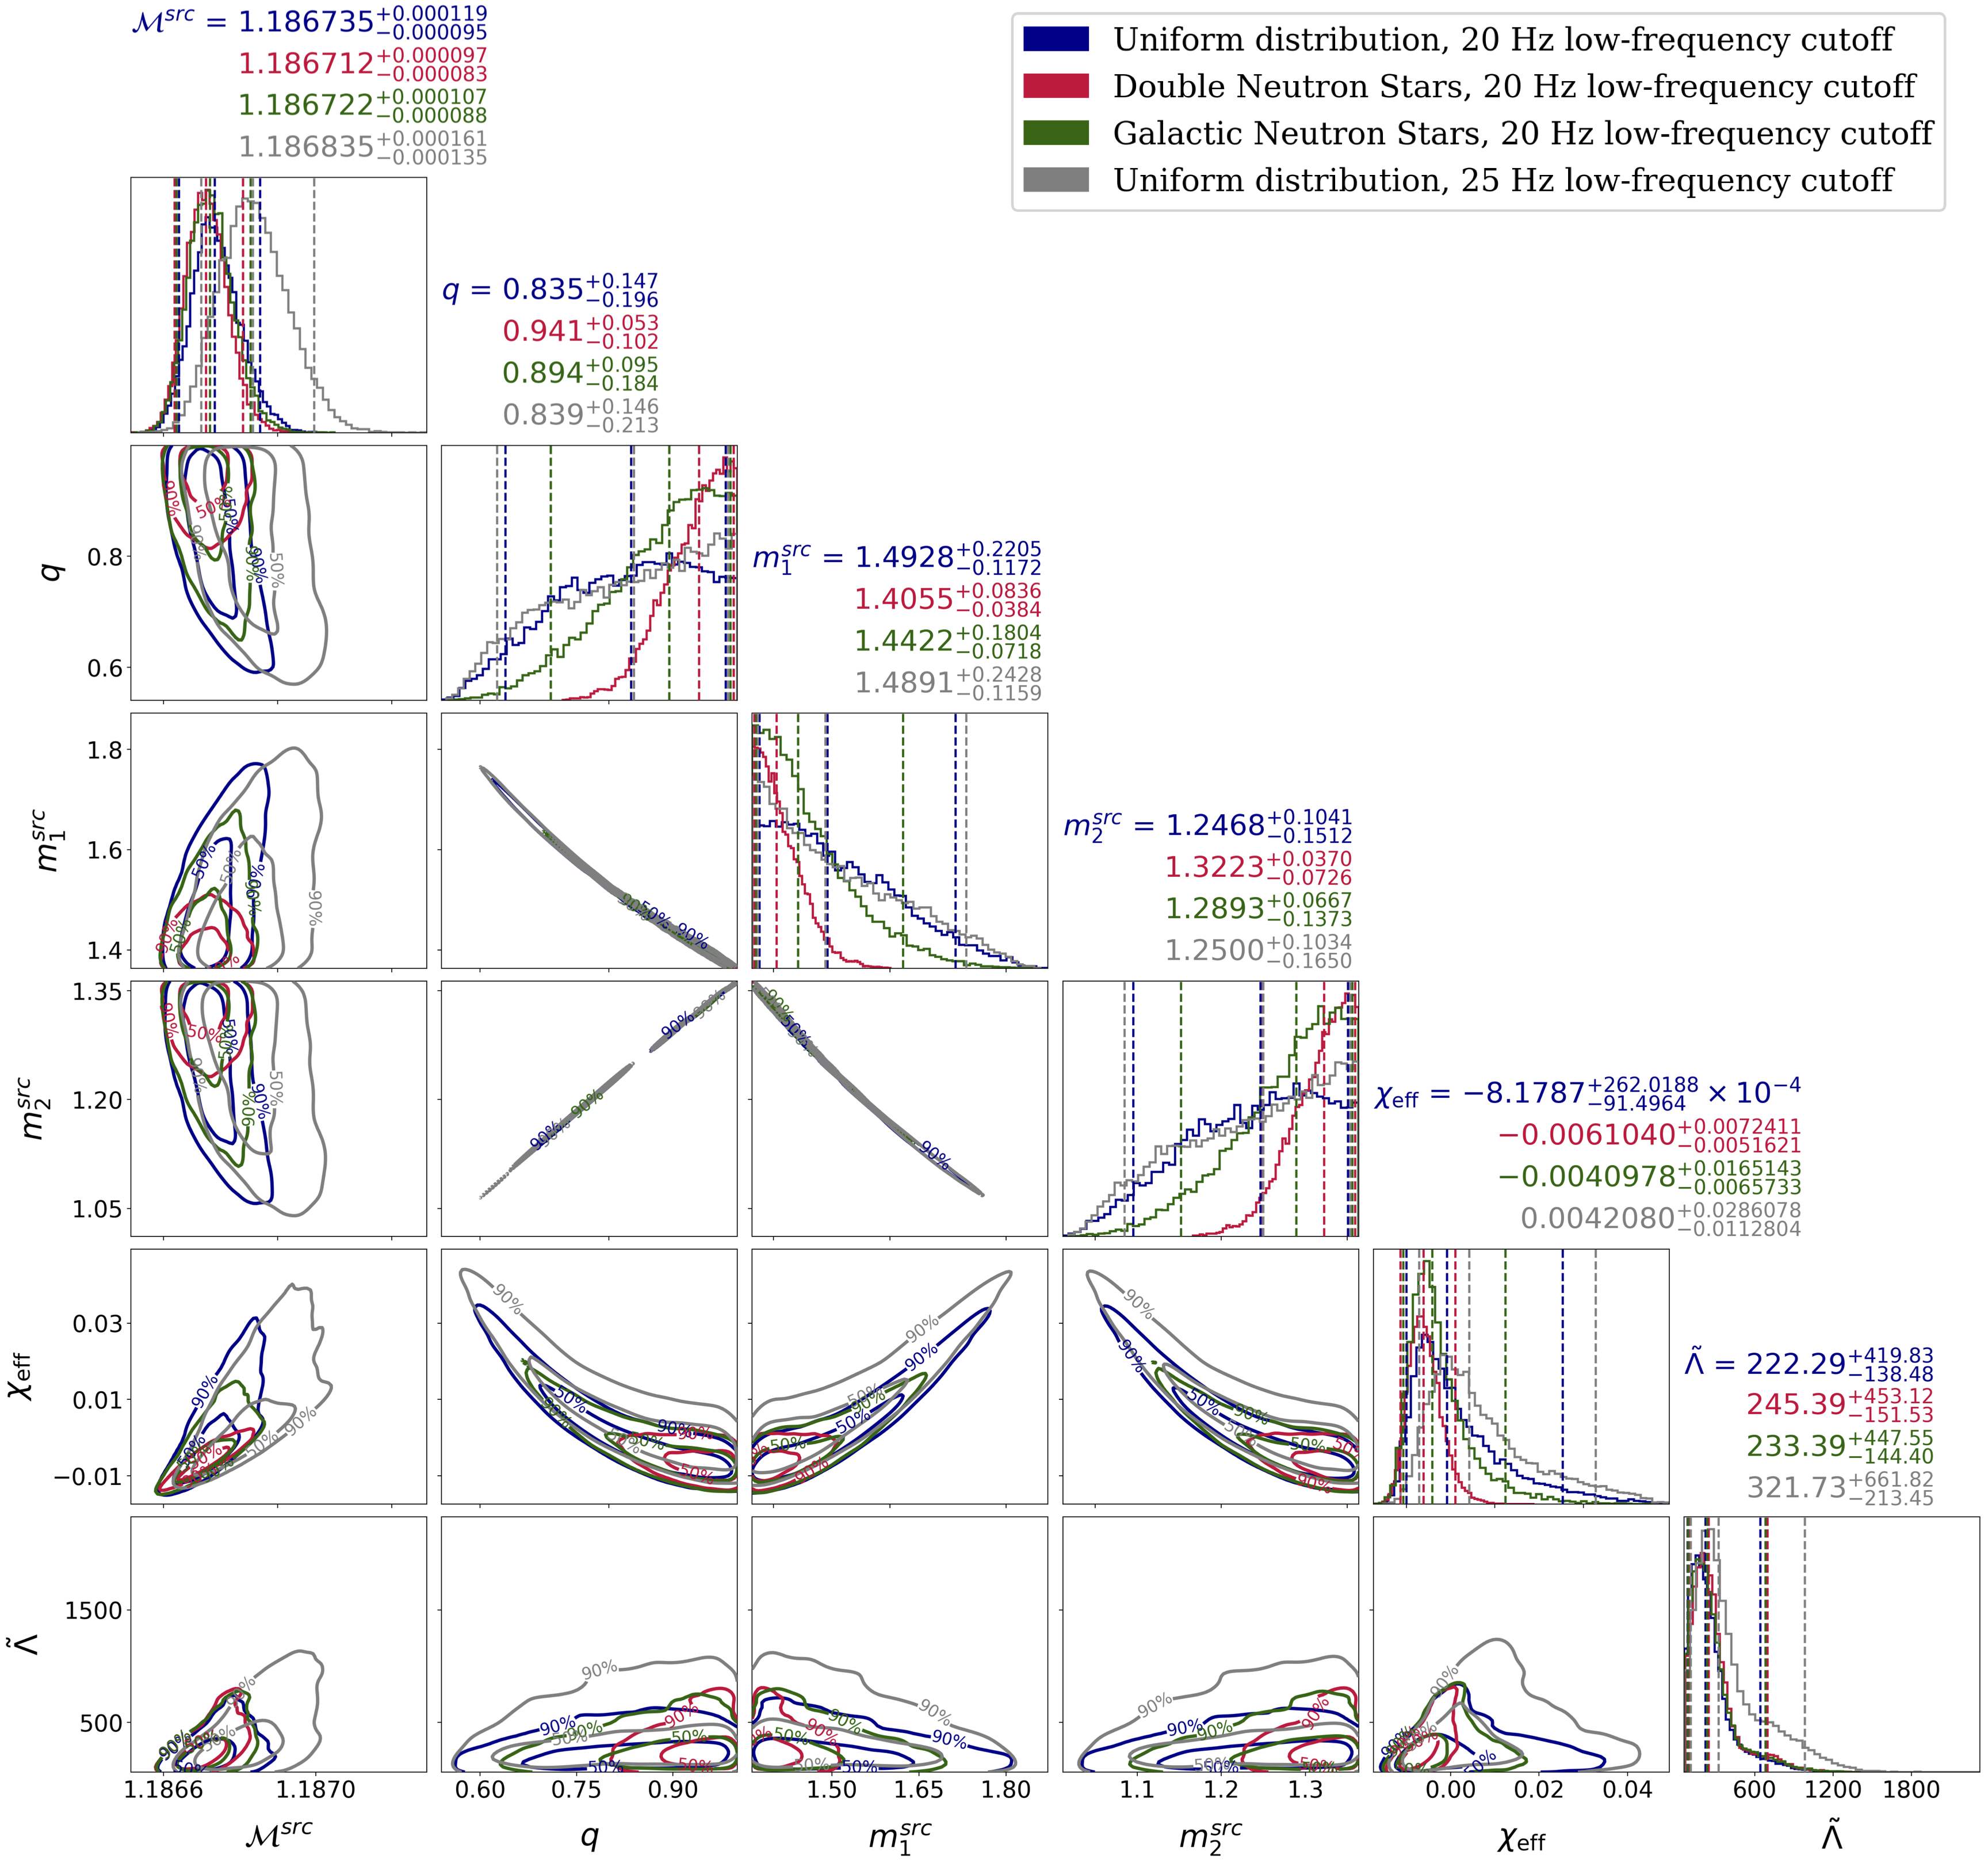
\includegraphics[width=\textwidth]{Figures/common-radius/posteriors_main_bothspins.png}
  \caption{\footnotesize Posterior distributions for the source frame chirp mass $\mathcal{M}^{\rm src}$, mass ratio $q$, source frame primary mass $m_1^{\rm src}$ and secondary mass $m_2^{\rm src}$, effective spin $\chi_{\rm eff}$, and binary deformability parameter $\tilde{\Lambda}$ from parameter estimation analyses with three different choices of mass priors. The posteriors represented in blue are from the analysis using a uniform prior on component masses, $m_{1,2} \sim U[1,2]\, M_\odot$, and 20~Hz low-frequency cutoff. The posteriors represented in red are from the analysis using a Gaussian mass prior for component masses $m_{1,2} \sim N(\mu = 1.33, \sigma = 0.09)\, M_\odot$ known from radio observations of neutron stars in double neutron star (DNS) systems, and 20~Hz low-frequency cutoff. The posteriors represented in green are from the analysis using the observed mass distributions of recycled and slow pulsars in the Galaxy with $m_1 \sim N(\mu = 1.54, \sigma = 0.23)\, M_\odot$ and $m_2 \sim N(\mu = 1.49, \sigma = 0.19)\, M_\odot$~\cite{Ozel:2016oaf}, and 20~Hz low-frequency cutoff. The posteriors represented in gray are from the analysis using a uniform prior on component masses, $m_{1,2} \sim U[1,2]\, M_\odot$, and 25~Hz low-frequency cutoff. All four analyses had the common EOS constraint and the causal $\Lambda(m)$ lower limit imposed. The one-dimensional plots show marginalized probability density functions for the parameters. The dashed lines on the one-dimensional histograms represent the 5$\%$, 50$\%$ and 95$\%$ percentiles for each analysis, the values of which are quoted in the titles of the histograms. The 2D plots show 50$\%$ and 90$\%$ credible regions for the different pairs of parameters. Comparison between the analyses with low-frequency cutoff 20~Hz (blue) and 25~Hz (gray) for the uniform mass prior case shows that extending from 25~Hz to 20~Hz better constrains $\mathcal{M}$, which improves the measurement of $\tilde\Lambda$ by eliminating a region of the posterior with higher values $\mathcal{M}$ and high $\tilde\Lambda$.
  \label{fig:posterior_overlap}}
\end{adjustwidth}
\end{figure}

Figure \ref{fig:lamb12_1abc} shows the posterior probability densities for $\Lambda_1$ and $\Lambda_2$ with 90\% and 50\% credible region contours. Overlaid are $q$ contours and $\tilde{\Lambda}$ contours obtained from Eq.~(\ref{eq:common_rad_lambda_t0}), $\Lambda~\simeq a\beta^{-6}$, and $R_1 \simeq R_2 \simeq \large \hat R$ as
\begin{equation}
\Lambda_1(\tilde{\Lambda},q)={\frac{13}{16}}\tilde{\Lambda}{\frac{q^2(1+q)^4}{12q^2-11q+12}},
\label{eq:l1l2}\quad \Lambda_2(\tilde{\Lambda},q) = q^{-6} \Lambda_1 .\end{equation}
Because of our constraint $\Lambda_2 \geq \Lambda_1$, our credible contours are confined to the region where $q \leq 1$. One can easily demonstrate that $\Lambda_2 \geq \Lambda_1$ is valid unless $(c^2/G)dR/dm > 1$, which is impossible for realistic equations of state. For the entire set of piecewise polytropes satisfying $m_\mathrm{max}>2M_\odot$ we considered, $(c^2/G)dR/dm$ never exceeded 0.26. Even if a first order phase transition appeared in stars with masses between $m_2$ and $m_1$, it would necessarily be true that $dR/dm < 0$ across the transition. Because of the $q$ dependence of $\Lambda_1$, $\Lambda_2$, the credible region enclosed by the contours broadens from the double neutron star (most restricted), to the pulsar, to the uniform mass (least restricted) priors. However, the upper bound of the credible region is robust.

We find $\tilde{\Lambda}=
205^{+415}_{-167}$ for the uniform component mass prior, $\tilde{\Lambda}=234^{+452}_{-180}$ for the prior informed by double neutron star binaries in the Galaxy, and $\tilde{\Lambda}=218^{+445}_{-173}$ for the prior informed by all Galactic neutron star masses (errors represent 90\% credible intervals). Our measurement of $\tilde{\Lambda}$ appears to be robust to the choice of component mass prior, within the (relatively large) statistical errors on its measurement. The Bayes factors comparing the evidence from the three mass priors are of order unity, so we cannot claim any preference between the mass priors.

The 90\% credible intervals on $\tilde{\Lambda}$ obtained from the gravitational-wave observations include regions forbidden by causality. Applying a constraint to our posteriors for the causal lower limit of $\Lambda$ as a function of $m$~\cite{Zhao:2018nyf}, we obtain $\tilde{\Lambda}=
222^{+420}_{-138}$ for the uniform component mass prior, $\tilde{\Lambda}=245^{+453}_{-151}$ for the prior informed by double neutron star binaries in the Galaxy, and $\tilde{\Lambda}=233^{+448}_{-144}$ for the prior informed by all Galactic neutron star masses (errors represent 90\% credible intervals). Using Eq.~(\ref{eq:rhat}), we map our $\cal{M}$ posteriors and $\tilde{\Lambda}$ posteriors (with the causal lower limit applied) to $\hat{R} \simeq R_{1.4}$ posteriors, allowing us to estimate the common radius of the neutron stars for GW170817 for each mass prior. Figure~\ref{fig:radius_lambda} shows the posterior probability distribution for the binary tidal deformation $\tilde\Lambda$ and the common radius $\hat{R}$ of the neutron stars in the binary. Our results suggest a radius $\hat R = 10.7^{+2.1}_{-1.6} \pm 0.2$ km (90\% credible interval, statistical and systematic errors) for the uniform mass prior,  $\hat R = 10.9^{+2.1}_{-1.6} \pm 0.2$ km for double neutron star mass prior, and $\hat R = 10.8^{+2.1}_{-1.6} \pm 0.2$ km for the prior based on all neutron star masses.

%For the uniform mass prior, we computed the Bayes factor comparing a model with a prior $\Lambda_s \sim U[0,5000]$ to a model with a prior $\Lambda_s \sim U[0,100]$. We find $\log_{10}(\mathcal{B}) \sim 1$, suggesting that the data favors a model that includes measurement of tidal deformability $\tilde\Lambda \gtrsim 100$. However, the evidences were calculated using thermodynamic integration of the MCMC chains~\cite{emcee}. We will investigate model selection using, e.g., nested sampling \cite{skilling2006} in a future work.

Finally, we note the post-Newtonian waveform family used will result in systematic errors in our measurement of the tidal deformability \cite{Wade:2014vqa,Lackey:2014fwa}. However, this waveform family allows a direct comparison to the results of Ref.~\cite{TheLIGOScientific:2017qsa}. Accurate modeling of the waveform is challenging, as the errors in numerical simulations are comparable to the size of the matter effects that we are trying to measure~\cite{Barkett:2015wia}. Waveform systematics and comparison of other waveform models (e.g., \cite{Bernuzzi:2014owa}) will be investigated in a future work.

\begin{figure}[t]
  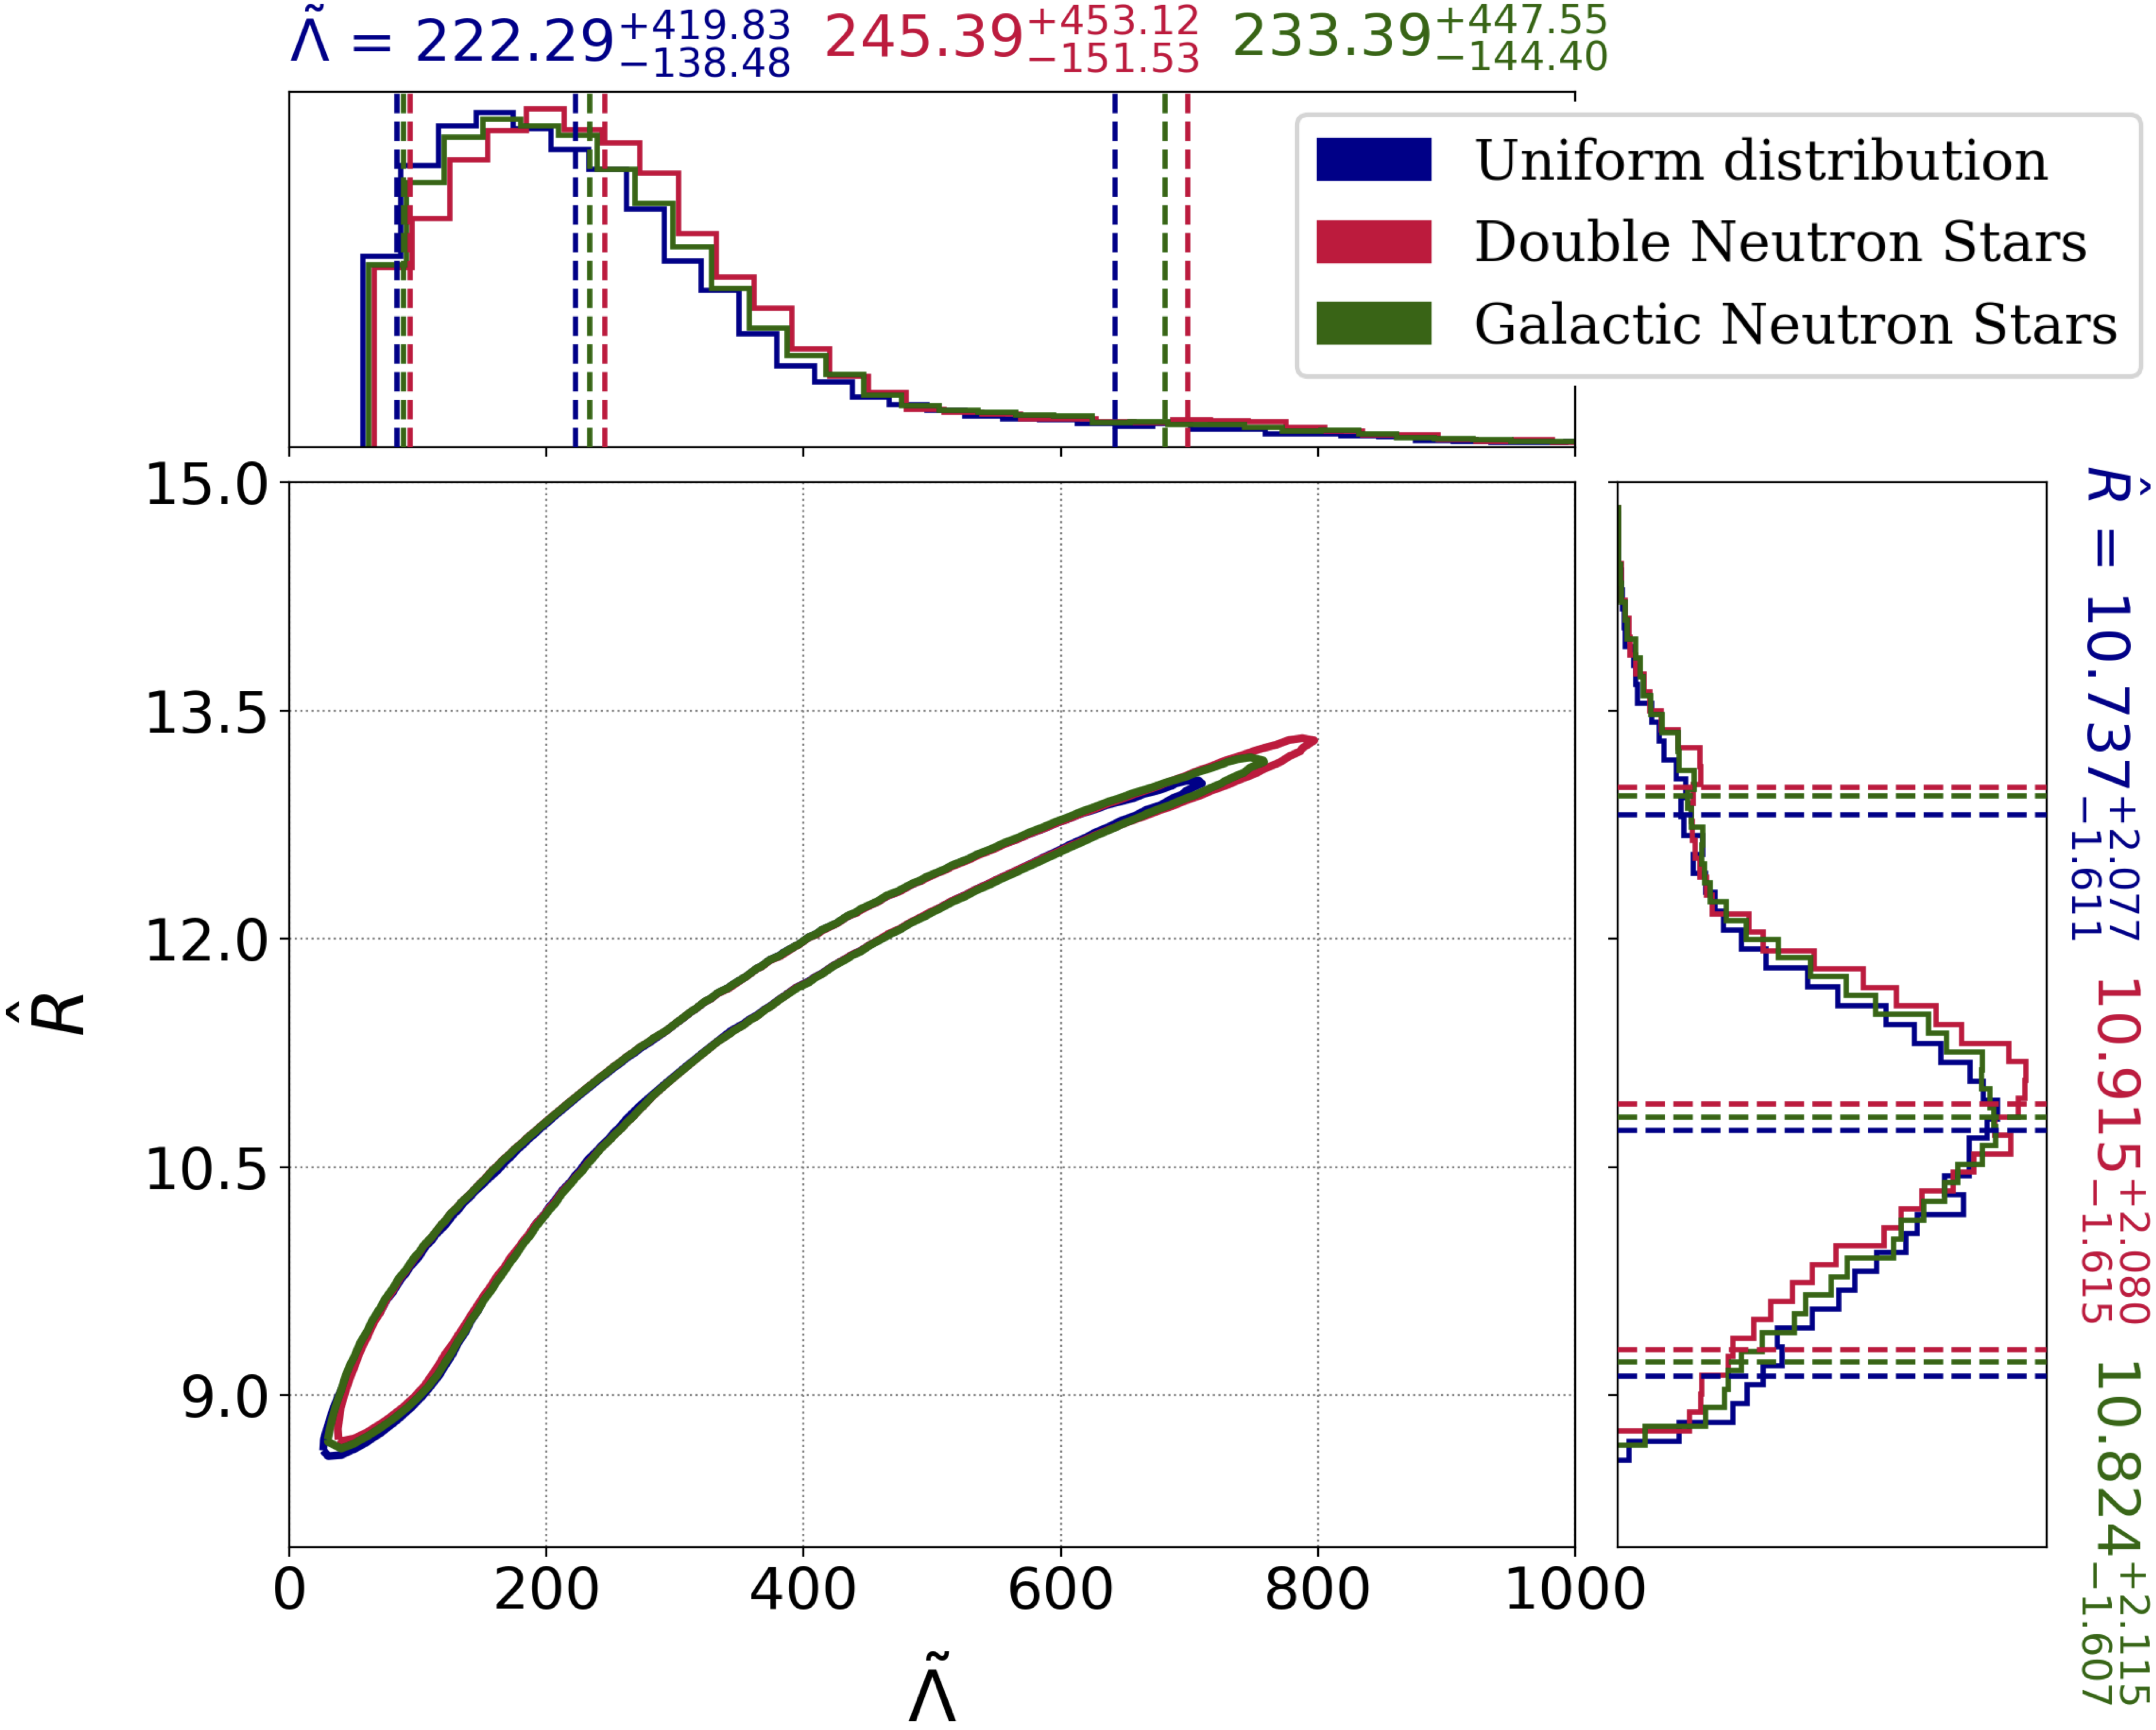
\includegraphics[width=\textwidth]{Figures/common-radius/Radius_lambda_bothspins.png}
  \caption{The 90\% credible region of the posterior probability for the common radius $\hat{R}$ and binary tidal deformability $\tilde\Lambda$ with the common EOS constraint for the three mass priors. The posteriors for the individual parameters are shown with dotted lines at  the 5$\%$, 50$\%$ and 95$\%$ percentiles. The values of $\tilde\Lambda$, and hence $\hat{R}$ forbidden by causality have been excluded from the posteriors. 
\label{fig:radius_lambda}%
%\vspace*{-0.5cm}%
}
\end{figure}

\section{Discussion}

Using Bayesian parameter estimation, we have measured the tidal deformability and common radius of the neutron stars in GW170817. Table~\ref{tab:summary_table} summarizes our findings.  To compare to Ref.~\cite{TheLIGOScientific:2017qsa}, which reports a 90\% upper limit on $\tilde\Lambda \le 800$ under the assumption of a uniform prior on $\tilde\Lambda$, we integrate the posterior for $\tilde{\Lambda}$ to obtain 90\% upper limits on $\tilde{\Lambda}$.   For the common EOS analyses, these are $485$, $521$, and $516$ for the uniform, double neutron star, and Galactic neutron star component mass priors, respectively. We find that, in comparison to the unconstrained analysis, the common EOS assumption significantly reduces the median value and 90\% confidence upper bound of $\tilde\Lambda$ by about 28\% and 19\%, respectively, for all three mass priors. The difference between our common EOS results for the three mass priors is consistent with the physics of the gravitational waveform. At constant $\mathcal{M}$, decreasing $q$ causes the binary to inspiral more quickly \cite{Hannam:2013uu}. At constant $\mathcal{M}$ and constant $q$, increasing $\tilde\Lambda$ also causes the binary to inspiral more quickly, so there is a mild degeneracy between $q$ and $\tilde\Lambda$. The uniform mass prior allows the largest range of mass ratios, so we can fit the data with a larger $q$ and smaller $\tilde\Lambda$. The double neutron star mass prior allows the smallest range of mass ratios, and so, a larger $\tilde\Lambda$ is required to fit the data, with the Galactic neutron star mass prior lying between these two cases. 

\begin{table}[t]\label{tab:parameters}
\setlength{\tabcolsep}{3.8pt}
\centering\begin{tabular}{lcccc} 
\hline
\rule{0pt}{3ex}%
Mass prior \quad & \quad $\tilde{\Lambda}$ \quad & \quad $\hat{R}$ (km) \quad & \quad $\tilde{\Lambda}_{90\%}$\quad \\\hline
\rule{0pt}{3ex}%
Uniform & 222$^{+420}_{-138}$ & 10.7$^{+2.1}_{-1.6}\pm 0.2$ & $< 485$\\
Double neutron star & 245$^{+453}_{-151}$ & 10.9$^{+2.1}_{-1.6}\pm 0.2$ & $< 521$ \\
Galactic neutron star & 
233$^{+448}_{-144}$ & 10.8$^{+2.1}_{-1.6}\pm 0.2$ & $< 516$ \\
\hline
\end{tabular}
\caption{Results from parameter estimation analyses using three different mass prior choices with the common EOS constraint, and applying the causal minimum constraint to $\Lambda(m)$. We show 90$\%$ credible intervals for $\tilde{\Lambda}$, 90$\%$ credible intervals and systematic errors for $\hat{R}$, and the 90\% upper limits on $\tilde\Lambda$.%
\vspace*{-0.5cm}%
}
\label{tab:summary_table}
\end{table}
Nevertheless, considering all analyses we performed with different mass prior choices, we find a relatively robust measurement of the common neutron star radius with a mean value $\langle \large \hat R \rangle$ = 10.8 km bounded above by $\hat R < 13.2$~km and below by $\hat R > 8.9$~km. Nuclear theory and experiment currently predict a somewhat smaller range by 2 km but with approximately the same centroid as our results~\cite{Lattimer:2012nd,Lattimer:2012xj}. A minimum radius 10.5--11 km is strongly supported by neutron matter theory~\cite{Gandolfi:2011xu,Lynn:2015jua,Drischler:2015eba}, the unitary gas~\cite{Kolomeitsev:2016sjl}, and most nuclear experiments~\cite{Lattimer:2012nd,Lattimer:2012xj,Tews:2012fj}. The only major nuclear experiment that could indicate radii much larger than 13 km is the PREX neutron skin measurement, but this has published error bars much larger than previous analyses based on antiproton data, charge radii of mirror nuclei, and dipole resonances. 
Our results are consistent with photospheric radius expansion measurements of x-ray binaries which obtain $R \approx 10$--$12$~km~\cite{Ozel:2016oaf,Steiner:2010fz,Degenaar:2018lle}. Reference~\cite{Guillot:2014lla} found from an analysis of five neutron stars in quiescent low-mass x-ray binaries a common neutron star radius $9.4\pm1.2$ km, but systematic effects including uncertainties in interstellar absorption and the neutron stars' atmospheric compositions are large. Other analyses have inferred $12\pm0.7$~\cite{Lattimer:2013hma} and $12.3\pm1.8$ km~\cite{Shaw:2018wxh} for the radii of $1.4M_\odot$ quiescent sources. 

We have found that the relation $q^{7.48} < \Lambda_1/\Lambda_2 < q^{5.76}$, in fact, completely bounds the uncertainty for the range of $\mathcal{M}$ relevant to GW170817, assuming $m_2 > 1M_\odot$ \cite{Zhao:2018nyf} and that no strong first-order phase transitions occur near the nuclear saturation density (i.e., the case in which $m_1$ is a hybrid star and $m_2$ is not). Analyses using this prescription instead of the $q^6$ correlation produce insignificant differences in our results. Since models with the common EOS assumption are highly favored over those without this assumption, our results support the absence of a strong first-order phase transition in this mass range.

We have shown that, for binary neutron star mergers consistent with observed double neutron star systems~\cite{Tauris:2017omb}, assuming a common EOS implies that $\Lambda_1 / \Lambda_2 \simeq q^6$. We find evidence from GW170817 that favors the common EOS interpretation compared to uncorrelated deformabilities. Although previous studies have suggested that measurement of the tidal deformability is sensitive to the choice of mass prior \cite{Agathos:2015uaa}, we find that varying the mass priors does not significantly influence our conclusions suggesting that our results are robust to the choice of mass prior. Our results support the conclusion that we find the first evidence for finite size effects using gravitational-wave observations. 

Recently, the LIGO/Virgo collaborations have placed new constraints on the radii of the neutron stars using GW170817~\cite{Abbott:2018exr}. The most direct comparison is between our uniform mass prior result ($\hat R = 10.7^{+2.1}_{-1.6} \pm 0.2$) and the LIGO/Virgo method that uses equation-of-state-insensitive relations~\cite{Yagi:2016qmr,Chatziioannou:2018vzf} ($R_1 = 10.8^{+2.0}_{-1.7}$ and $R_2 = 10.7^{+2.1}_{-1.5}$~km). This result validates our approximation $R_1=R_2$ used to motivate the prescription $\Lambda_1=q^6\Lambda_2$, and Eqs.~(\ref{eq:lambda_t1}, \ref{eq:lambda_t2}). Our statistical errors are comparable to the error reported by LIGO/Virgo. Systematic errors from EOS physics of $\pm 0.2$~km are added as conservative bounds to our statistical errors, broadening our measurement error, whereas Ref.~\cite{Abbott:2018exr} marginalized over these errors in the analysis. Reference~\cite{Abbott:2018exr} also investigates a method of directly measuring the parameters of the EOS which results in smaller measurement errors. Investigation of these differences between our analysis and the latter approach will be pursued in a future paper. 

Observations of future binary neutron star mergers will allow further constraints to be placed on the deformability and radius, especially if these binaries have chirp masses similar to GW170817 as radio observations suggest. As more observations improve our knowledge of the neutron star mass distribution, more precise mass-deformability correlations can be used to further constrain the star's radius.




\Chapter{Prospects for Precise Equation of State Measurements from Advanced LIGO and Cosmic Explorer}
\label{ch:eos-meas}
Neutron star mergers probe the nature of matter at densities and temperatures far beyond those available in the laboratory. 
The observation of GW170817 confirmed that gravitational waves can yield meaningful insights into the structure of neutron stars, and hence on the equation of state of matter above nuclear density~\cite{TheLIGOScientific:2017qsa,De:2018uhw,Fattoyev:2017jql,Tews:2018iwm,Margalit:2017dij,Annala:2017llu,Raithel:2018ncd}. Combining gravitational-wave and electromagnetic observations of the first neutron star merger with nuclear theory and numerical simulations has already shed new light on the equation of state of dense matter~\cite{Capano:2019eae,Dietrich:2020efo,AlMamun21}.
The ability of multi-messenger observations of merging neutron stars to
explore nuclear physics is determined by: the signal-to-noise ratio of the observed
gravitational-wave signals; the fidelity of the waveforms used 
to model gravitational-wave signals; the ability to model and extract 
information from electromagnetic counterparts; and
theoretical modeling of hot and cold dense nuclear matter and its 
connection to the observed quantities. In this chapter, we focus on the impact that the signal-to-noise
ratio of the signal has on the ability to measure the neutron star equation of state with current and future gravitational-wave detectors.

Gravitational-wave observations of binary neutron star mergers measure the nuclear equation of state through the star's tidal deformability $\Lambda$ which is imprinted on the phasing of the inspiral waveform. This measurement of $\Lambda$ is equivalent to a measurement of the neutron star radius, and hence the nuclear equation of state which connects these two quantities for a given mass. Previous studies have shown that Advanced LIGO will be able to measure the radius of a 1.4\msun~neutron star $R_{1.4}$ to better than 10\% precision with the first few tens of binary neutron star signals. However many plausible equations of state produce similar radii for a range of masses, so that distinguishing between them would require measurement precision better than 2\%. In this work we assess the ability of both Advanced LIGO and the proposed third-generation detector Cosmic Explorer, to make a precise measurement of the equation of state from a large population of simulated binary neutron star signals, for several equations of state that span the plausible range. We perform full Bayesian parameter estimation on all simulated signals and produce a combined measurement of $R_{1.4}$. We find that with 321 signals Advanced LIGO is able to measure $R_{1.4}$ to better than 2\% across the entire range of plausible equations of state, although the probability of seeing so many signals in the next decade is low. On the other hand we find that with one year of observation, Cosmic Explorer will be able to measure $R_{1.4}$ to within 0.6\% for a soft equation of state, and to within 0.15\% for a moderately stiff equation of state.

\section{Introduction}
The observation of the binary neutron star merger GW170817 during the second observing run of the LIGO-Virgo network provided the first constraints on the cold dense matter equation of state through gravitational waves~\cite{LIGOScientific:2017vwq}. The observations of AT2017gfo, the electromagnetic counterpart to GW170817, were also able to constrain the equation of state through estimates of the ejecta mass and velocity~\cite{Radice:2018ozg}, and by probing the fate of the merger remnant~\cite{Margalit:2019dpi}. Additional constraints have also recently come from pulsar observations and nuclear experiment: X-ray observations by the \textit{NICER} instrument of the pulsars J0740$+$6620 and J0030$+$0451 have mapped out some of the neutron star mass-radius relationship through direct radius measurements~\cite{Riley:2019yda,Riley:2021pdl,Miller:2021qha}, and in the low pressure regime the \textit{PREX-II} experiment has made precise measurements of the density dependence of the nuclear symmetry energy for lead atoms~\cite{PREX:2021umo}, which can be mapped to the higher pressures in neutron stars in order to also provide an estimate of the expected neutron star radius~\cite{Reed:2021nqk}. Recent efforts have been made to combine some of these and other disparate measurements into a generalized constraint on the equation of state, often given in terms of the radius of a 1.4\msun~neutron star $R_{1.4}$: \cite{Reed:2021nqk} combined the \textit{PREX-II} measurement and the \textit{NICER} constraints on the radius of the pulsar J0030$+$0451 to give $13.25~\mathrm{km}<R_{1.4}<14.26~\mathrm{km}$ (1$\sigma$ limits), and \cite{Al-Mamun:2020vzu} combined GW170817, quiescent low-mass X-ray binaries, photospheric radius expansion X-ray bursts, and J0030$+$0451 to find $R_{1.4}=11.83_{-0.71}^{+0.62}$~km (2$\sigma$ limits).

% P2 negative on current constraints
While great strides have been made in producing constraints on the equation of state, the prospects for improving these constraints using binary merger events still face significant challenges. GW170817 was a remarkably loud signal, with a signal-to-noise ratio of over 33, and yet the gravitational-wave observation alone was insufficient to conclusively distinguish the signal from a pair of merging black holes~\cite{LIGOScientific:2017vwq}. A second binary neutron star signal, GW190425, was observed by the LIGO-Virgo network but at a much lower signal-to-noise ratio of 13, which provided negligible information about the equation of state and also meant that no electromagnetic counterpart was identified~\cite{LIGOScientific:2020aai}. Similarly, there have been three gravitational-wave observations of probable neutron star--black hole mergers to date containing no measurable information on the equation of state, or any identifiable electromagnetic counterpart from the possible disruption of the neutron star~\cite{LIGOScientific:2020zkf,LIGOScientific:2021qlt}. Further complicating matters, the estimated merger rate of binary neutron stars in the local universe has been revised significantly lower after the completion of LIGO's third observing run~\cite{Abbott:2020gyp}, which means a correspondingly lower probability that future observing runs will produce a large set of observed signals that can be combined into a precise constraint on the equation of state.

% Add that SQM3, WFF2, and APR4 predict similar R_1.4 
Where previous works have investigated distinguishability between equation of state models, most have primarily focused on distinguishing models that differ substantially from one another. However many models exist that are consistent with current constraints but make similar predictions. As an example, the commonly used models WFF2, APR4, and SQM3, predict values for $R_{1.4}$ of 11.16, 11.32, and 11.37 kilometers, respectively. Naturally the prospect of distinguishing between these or other similar models is a much greater challenge, but this is very likely what will be required of future equation of state constraints. For the example models given, this will require measurements of $R_{1.4}$ with a precision better than 2\%.

% P3 why soft EOS is hard
The ability to measure the equation of state in gravitational-wave signals depends very sensitively on the equation of state itself, because the range of plausible models predict varying amounts of information in an inspiral waveform. Gravitational-wave signals from coalescing neutron stars carry information about the equation of state as a result of the tidal deformation that the stars' gravitational fields produce in one another. Specifically, the quadrupole moment $Q_{ij}$ of one neutron star is related to the tidal field $\mathcal{E}_{ij}$ of the other neutron star according to $Q_{ij} = -\lambda\mathcal{E}_{ij}$, where $\lambda$ is the tidal deformability of the neutron star~\cite{Flanagan:2007ix}. The tidal deformability is dependent on the equation of state and is commonly expressed in dimensionless form as
\begin{equation}
    \Lambda=\frac{2}{3}k_{2}\left(\frac{Rc^{2}}{Gm}\right)^5
\end{equation}
where $k_{2}$ is the tidal Love number. $R$ and $m$ are the radius and mass of the neutron star, respectively. The energy expended in deforming the stars results in a phase difference in the gravitational waveform as compared to a signal with non-deforming bodies. An equation of state that has a large $\Lambda$ for a given mass is said to be ``stiff", and will generally correspond to a larger radius as the neutron star is more able to hold itself up against gravity. A stiff equation of state produces a larger effect on the gravitational-wave phasing and is therefore more measurable. Conversely, a ``soft" equation of state will have a smaller $\Lambda$ and radius for a given mass, and produces a less measurable effect in a gravitational-wave signal.

% P4 lit review of forecasts
Given the difficulty of measuring the equation of state, an established method of improving constraints is to combine multiple observations in order to reduce statistical uncertainty~\cite{DelPozzo:2013ala}. Previous works have used various implementations of this method to estimate the measurability of the equation of state for a given signal population or detector network~\cite{DelPozzo:2013ala,Lackey:2014fwa,Agathos:2015uaa,Vivanco:2019qnt,Pacilio:2021jmq}. Lackey and Wade \cite{Lackey:2014fwa} combined signals in a simulated LIGO-Virgo network at design sensitivity, for several choices of equation of state. They constrain the neutron star radius across a range of masses and find that the radius can be measured to within $\pm1$ kilometer with 20 signals. Agathos {\it et al.}~\cite{Agathos:2015uaa} combined 200 signals in a LIGO-Virgo network and found that a catalog of at least 100 signals is sufficient to distinguish between soft, moderate, and stiff equations of state if one assumes perfect knowledge of the mass distribution, while 150 or more signals would be needed if the mass distribution was unknown. \cite{Vivanco:2019qnt} project that the 8 loudest signals from a population of 20 in a LIGO-Virgo network will constrain the radius of a canonical 1.4\msun neutron star to within 10\%. Pacilio {\it et al.}~\cite{Pacilio:2021jmq} combine 20 signals in both a LIGO-Virgo network and Einstein Telescope, a proposed third-generation detector. They find that LIGO-Virgo is unable to distinguish between similarly soft equations of state from a catalog of 12 used in the analysis, although Einstein Telescope can potentially make this distinction.

% P5 overview of results and method
In this chapter we build upon these previous works to produce an accurate forecast for a high precision measurement of the equation of state, using both a LIGO-Virgo network operating at design sensitivity as well as a planned third-generation detector Cosmic Explorer. We make our forecast using a population of simulated binary neutron star signals generated from astrophysically realistic parameter distributions. We produce parallel populations of these signals for three choices of equation of state that span the range of the most up-to-date constraints from gravitational-wave events, electromagnetic observations of pulsars and the kilonova AT2017gfo, and nuclear experiments. We perform full Bayesian parameter estimation for each signal in our populations to recover the intrinsic and extrinsic source parameters, and we use a collection of 2000 realistic equations of state built from nuclear theory as a prior distribution in our analysis. We produce a combined equation of state measurement across our populations by transforming each measurement to a constraint on $R_{1.4}$, the radius of a 1.4\msun~neutron star. We find that a LIGO-Virgo network is able to measure $R_{1.4}$ to within 2\% across the entire range of plausible equations of state, though a soft equation of state will require significantly more signals that are unlikely to occur within the next planned observing runs. We find also that an incorrect mass prior used by our LIGO-Virgo analysis introduces a bias in the equation of state measurement such that a combined measurement with better than 2\% precision will exclude the true equation of state at high confidence. We find that Cosmic Explorer is able to achieve better than 0.6\% precision on $R_{1.4}$ with signals representing one year of observations for even the softest equation of state in our analysis. We find that in our Cosmic Explorer analysis an incorrect mass prior did introduce a bias, although it was not large enough to strongly exclude the true equation of state even with the much smaller statistical uncertainty on the measurement.

% P6
The rest of this chapter is organized as follows: Section~\ref{sec:population} describes the simulated binary neutron star signals included in our analysis. In Section~\ref{sec:eos} we give background information on equation of state information in gravitational-wave inspiral signals and describe the equations of state used in this analysis. Section~\ref{sec:eos_meas_pe} gives details about our parameter estimation analysis including the method of combining measurements. Section~\ref{sec:eos_meas_results} presents the results of our analysis including constraints for each of our chosen equations of state. Finally, we conclude in Section~\ref{sec:eos_meas_conclusion}.

\section{Simulated signals}\label{sec:population}

To simulate measurement scenarios for a LIGO-Virgo network and Cosmic Explorer, we generate a population of simulated binary neutron star merger signals and project them onto the corresponding detectors. For LIGO-Virgo we simulate a three-detector network representing the LIGO Hanford, LIGO Livingston~\cite{TheLIGOScientific:2016agk,Buikema:2020dlj}, and Virgo~\cite{TheVirgo:2014hva} detectors. Each LIGO-Virgo detector is simulated at its design sensitivity by injecting simulated signals into Gaussian noise colored by the design power spectral density for each detector~\cite{Aasi:2013wya}. Cosmic Explorer is still in its design phase and does not have a final configuration or site location determined yet, although potential sites in the United States include locations in Utah or Idaho. For simplicity we use a hypothetical Cosmic Explorer detector at the same location and orientation as the LIGO Hanford detector. We choose the 40 kilometer arm length configuration optimized for detection of coalescing binaries for our analysis, and signals are injected into Gaussian noise colored by the corresponding design power spectral density~\cite{CE:NoiseCurves}.

% parameter distributions
Following the prescription of \cite{Agathos:2015uaa} we generate our simulated binary neutron star mergers using astrophysically motivated distributions for the source parameters. The collection of electromagnetic observations of known galactic pulsars has found their mass distribution to be well described by a Gaussian centered near 1.4\msun. However the gravitational wave observations of GW190425 and two of the neutron star--black hole signals show evidence for a greater number of high-mass neutron stars in the range $1.7-1.9$\msun. To account for both possibilities and to investigate the effect of a different mass distribution on the ability to measure the equation of state, we generate our population for two choices of mass distribution. For our primary population, source-frame component masses are drawn from a Gaussian distribution with mean $\mu_{m}=1.4$\msun~and standard deviation $\sigma_{m}=0.05$\msun. A secondary population has source-frame component masses drawn uniformly in the range $1-2$\msun. In all cases, component spins along the axis of orbital angular momentum are drawn from a Gaussian distribution with zero-mean and standard deviation $\sigma_{\chi}=0.02$. Sky locations are distributed uniformly across the sky, and the inclination and orientation of the binary systems is distributed uniformly on the sphere. For signals analyzed with the LIGO-Virgo network, distances are drawn uniformly in volume in the range [20, 585] Mpc, where the upper bound is the largest distance at which an optimally oriented binary merger with equal masses of 2\msun~would produce a single detector signal-to-noise ratio of 8. Simulated signals are then pre-filtered via a network matched-filter signal-to-noise calculation to select the subset with signal-to-noise $\rho_{\mathrm{mf}}>13.85$, which is equivalent to a signal-to-noise of 8 in each detector. The resulting LIGO-Virgo population contains 321 signals with signal-to-noise ratios that range from about 10 to 73 for the Gaussian-mass case, and 312 signals with signal-to-noise 10 to 65 for the uniform-mass case. For signals analyzed with Cosmic Explorer, distances are drawn uniformly in volume in the interval [20, 1100] Mpc, with the upper bound determined similarly to the LIGO-Virgo case except requiring $\rho_{\mathrm{mf}}>100$. The Cosmic Explorer population contains 335 signals with signal-to-noise ranging from about 97 to 790. Except where otherwise noted, stated results will be for the primary population.

We replicate our populations for three different equations of state, which are chosen to span the range allowed by the most comprehensive set of observations and constraints currently available. Each sub-population is generated using a single equation of state, and every neutron star within a sub-population has its tidal deformability determined by the equation of state and its mass. Our choices of equation of state are discussed in greater detail in Section~\ref{sec:eos}.
% state approximant used
All simulated signals are generated using the \texttt{IMRPhenomD\_NRTidal} waveform approximant~\cite{Husa:2015iqa,Khan:2015jqa,Dietrich:2017aum}, which is a frequency domain waveform available in LALSuite~\cite{2020ascl.soft12021L}. The waveform uses a phenomenological model tuned to numerical relativity data, and it includes contributions to the gravitational-wave phase due to the tidal deformation of the neutron stars.

\section{Equation of state in gravitational waves}\label{sec:eos}

A general frequency-domain gravitational waveform can be expressed
\begin{equation}
    h(f)=\mathcal{A}f^{-7/6}\exp[i(\psi_{pp}+\psi_{tidal})]
\end{equation}
where $\mathcal{A}$ is the waveform amplitude, $\psi_{pp}$ is the point-particle contribution to the phasing, and $\psi_{tidal}$ is the contribution to the phasing from tidal effects. At leading order, the tidal phasing is determined by the \emph{effective} tidal deformability $\tilde\Lambda$, defined as
\begin{equation}
    \tilde\Lambda=\frac{16}{13}\frac{(12q+1)\Lambda_{1}+(12+q)q^{4}\Lambda_{2}}{(1+q)^{5}}
\end{equation}
where $q=m_{2}/m_{1}\leq1$ is the mass ratio. Thus the leading order tidal phasing in a gravitational waveform is
\begin{equation}\label{eq:tidal_phase}
    \psi_{tidal} \propto \tilde\Lambda f^{5/3}.
\end{equation}
This means a gravitational-wave signal allows a measurement of the amount of deformation occurring during an inspiral, and thus of the equation of state of the dense matter comprising the interior of the neutron star.
As is clear from Equation~\ref{eq:tidal_phase} the tidal effect in a gravitational waveform is larger for higher frequencies, and it has previously been found that it only becomes measurable for $f\gtrsim400$ Hz~\cite{Harry:2018hke}. Both the LIGO-Virgo and proposed Cosmic Explorer detectors have decreased sensitivity at these higher frequencies where the tidal information exists, due to fundamental limitations of the laser interferometer design~\cite{Caves:1981hw}. This makes the measurement of tidal information in gravitational-wave signals inherently challenging, and therefore differences in measurability between soft and stiff equations of state can be significant.

To illustrate the issue, in Figure~\ref{fig:tidal_phase} we show the match between gravitational waveforms with tidal information included versus corresponding waveforms with no tides, where the match is measured as the noise-weighted overlap between the two waveforms. We calculate the match for different combinations of $\tilde\Lambda$ and neutron star mass $m$ for the case of an equal-mass binary. We plot also the functional $m-\Lambda$ relationship for two equations of state representing the soft and stiff ends of the plausible range. The measurability of the tidal information is equivalent to the degree of mismatch as compared to a non-tidal waveform. Both equations of state pass through regions of differing match owing to the mass dependence of the tidal deformability, but the stiff equation of state consistently lies in regions with substantially lower match implying a greater measurability. This is especially true for neutron star masses below about 1.6\msun.

\begin{figure}[b]
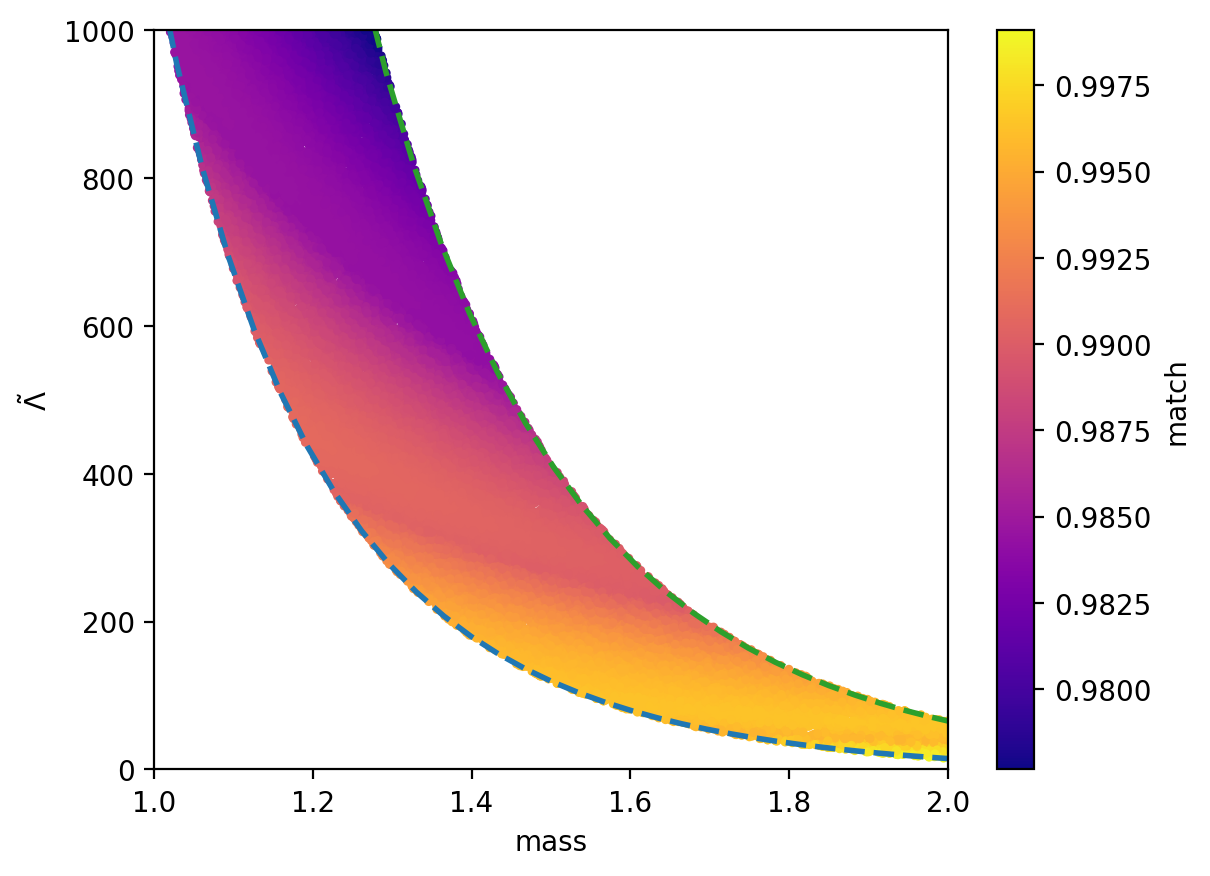
\includegraphics[width=\textwidth]{Figures/eos-meas/eos_match.png}
\caption{Match between gravitational waveforms for equal mass binaries with and without tidal deformability included. The match is calculated as the noise-weighted overlap between the two waveforms in the frequency range $20-2048$ Hz using the Advanced LIGO design sensitivity noise curve \texttt{aLIGODesignSensitivityP1200087}. Waveforms are generated using masses ranging from $1-2$\msun, and for the waveform including tidal deformability we use values of $\tilde\Lambda=\Lambda_{1}=\Lambda_{2}$ that span the range of plausible values between the soft (lower curve) and stiff (upper curve) equations of state selected for our analysis.}
\label{fig:tidal_phase}
\end{figure}

To explore the effect of a stiff or soft equation of state on our ability to place precise constraints, we select for our analysis three equations of state that span the full plausible range. We require that each equation of state support a maximum neutron star mass of 2\msun. For simplicity, we do not include any equations of state that contain a phase transition of the dense matter. The equations of state are selected from a set of 2000 that are constructed from nuclear chiral effective field theory, which is calibrated to nuclear experiments up to the nuclear saturation density. From soft to stiff, our chosen equations of state are labeled EOS 487, EOS 895, and EOS 1250, and in Figure~\ref{fig:eos_with_constraints} we show their location in the $R_{1.4}-\Lambda_{1.4}$ plane along with a selection of recent equation of state constraints from electromagnetic and gravitational-wave observations to date. Also plotted are the pairs of ($R_{1.4}$, $\Lambda_{1.4}$) values from the entire set of 2000 equations of state used in our analysis as a prior distribution for the parameter estimation, which we discuss in greater detail in Section~\ref{sec:eos_meas_pe}.

\begin{figure}[ht]
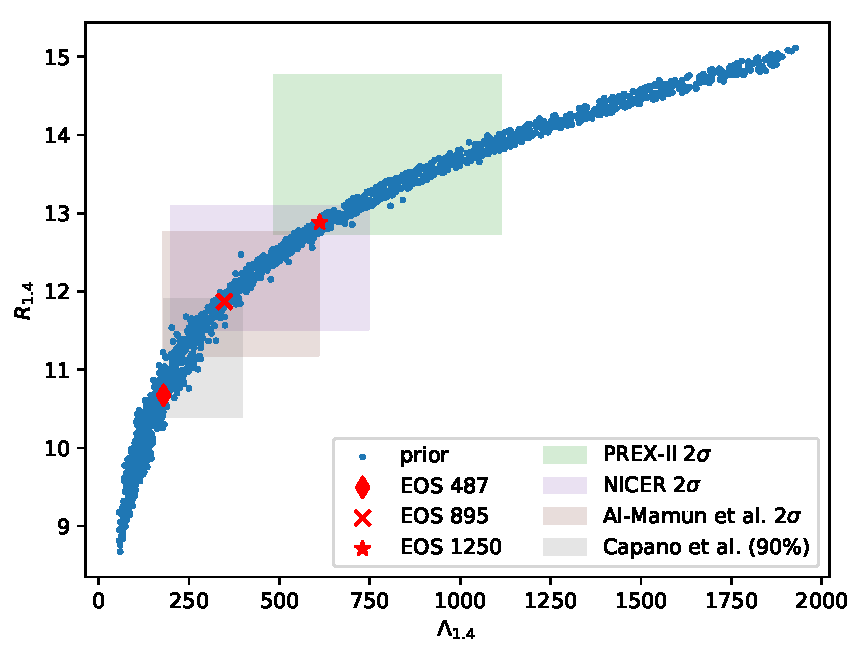
\includegraphics[width=\textwidth]{Figures/eos-meas/nsat_radius_vs_lambda.pdf}
\caption{
The radius in kilometers and dimensionless tidal deformability of a 1.4\msun\ neutron star, denoted $R_{1.4}$ and $\Lambda_{1.4}$, for the equations of state used in this work. The soft, medium, and stiff equations of state whose measurability we assess, EOS 487, EOS 895, and EOS 1250, are shown as a red diamond, red cross, and red star, respectively. The ($\Lambda_{1.4}, R_{1.4}$) coordinates for the 2000 equations of state used as a prior distribution in our analysis are shown in blue. Shaded regions represent a selection of constraints on the equation of state from gravitational-wave and electromagnetic observations, and nuclear experiment. The constraints span a significant range with potentially some tension between them. The three equations of state we investigate in this work are chosen to span the majority of the range covered by these constraints.
}
\label{fig:eos_with_constraints}
\end{figure}

\section{Parameter estimation}\label{sec:eos_meas_pe}

% Bayesian inference boilerplate
In general, under the assumption of Gaussian noise characterized by a power spectral density $S(f)$, the likelihood of obtaining detector data $d$ given the presence of a gravitational waveform $h(\theta)$ is
\begin{equation}
    \mathcal{L}(d|\theta)\propto\exp\left[-\frac{1}{2}\left<d-h(\theta)|d-h(\theta)\right>\right],
\end{equation}
where
\begin{equation}
    \left<a|b\right>=4\mathfrak{R}\int_{f_{\mathrm{min}}}^{f_{\mathrm{max}}}\frac{\tilde{a}^{*}(f)\tilde{b}(f)}{S(f)}df
\end{equation}
is the noise-weighted inner product~\cite{Finn:1992xs,Chernoff:1993th} and $\theta= \left\{ \theta_{1},\theta_{2},\ldots,\theta_{n} \right\}$ is the set of intrinsic and extrinsic parameters defining the waveform.
In evaluating this likelihood, we can obtain estimates of the gravitational-wave parameters $\theta$ through the joint posterior probability distribution
\begin{equation}
    p(\theta|d)\propto\mathcal{L}(d|\theta)p(\theta),
\end{equation}
where $p(\theta)$ is the assumed prior probability distribution of the parameters. Then the marginal posterior probability distribution for an individual parameter is obtained by integrating $p(\theta|d)$ over all nuisance parameters. For instance, the marginalized posterior distribution for $\theta_{1}$ is
\begin{equation}
    p(\theta_{1}|d)=\int p(\theta|d)~\mathrm{d}\theta_{2}\mathrm{d}\theta_{3}\ldots\mathrm{d}\theta_{n}.
\end{equation}

We use \textit{PyCBC Inference}~\cite{Biwer_2019} with the parallel-tempered version of the \texttt{emcee} sampler~\cite{Foreman_Mackey_2013,Vousden_2015,2010CAMCS...5...65G} to sample the parameter space and produce marginalized posterior distributions for the source parameters. To help speed convergence we employ the relative likelihood model available in \textit{PyCBC Inference} which uses an approximation to the full resolution likelihood near its peak in order to reduce run-time, and has been shown to produce comparable parameter estimates to non-relative models~\cite{Cornish:2010kf,Zackay:2018qdy,Finstad:2020sok}. For signals analyzed in the LIGO-Virgo network we include frequencies above a low-frequency cutoff of 20 Hz, and for Cosmic Explorer signals we use frequencies above 7 Hz. All signals are analyzed up to a high frequency cutoff of 2048 Hz.
% describe priors
We sample in source-frame component masses, component spins along the direction of the orbital angular momentum, sky location, distance, geocentric time of coalescence, inclination, polarization angle, and equation of state. For each parameter we use a prior distribution that matches the corresponding population distribution with the exception of the equation of state, where our prior distribution is made of a collection of 2000 equations of state built from nuclear theory and designed to be roughly uniform in $R_{1.4}$ over the interval $9-15$ kilometers. Each equation of state provides a mapping between mass, radius, and tidal deformability for a neutron star. At each iteration, a single equation of state is drawn and used to determine the tidal deformabilities of both neutron stars based on their source-frame masses. In generating a template waveform for the likelihood, source-frame masses are first converted to the detector frame through scaling by a factor of $(1+z)$, where $z$ is the cosmological redshift at the sampled distance assuming a flat $\Lambda$CDM cosmology. All template waveforms are generated using the \texttt{IMRPhenomD\_NRTidal} waveform in order to match the simulated signals and avoid any systematic errors arising from different implementations across waveform families.

%\subsection{Event combination}

Multiple signals $s_{1},s_{2},\ldots,s_{N}$ are considered independent of one another and thus the posterior distributions for a given parameter $\theta_{k}$ can be combined straightforwardly across all signals~\cite{DelPozzo:2013ala,Agathos:2015uaa}
\begin{equation}
    p(\theta_{k}|s_{1},s_{2},\ldots,s_{N})=p(\theta_{k})^{1-N}\prod_{i=1}^{N} p(\theta_{k}|s_{i})
\end{equation}
where we have assumed the prior $p(\theta_{k})$ is the same for all signals. 

\section{Results}\label{sec:eos_meas_results}

In order to combine measurements across an entire population, we transform the posteriors of the equation of state for all signals to posteriors of a common parameter, $R_{1.4}$. Then each signal we analyze constitutes an independent measurement of the same physical quantity, and we can combine posterior distributions across many events following the procedure outlined in the previous section. To simulate a scenario of cumulatively combining each new signal as it occurs, we combine $R_{1.4}$ posteriors one at a time to track the radius constraint (as measured by the 90\% credible interval width) as a function of the number of signals included. This also allows for a straightforward conversion to constraint over time, given a merger rate and detector network sensitivity.

% aLIGO default results
For the 321 signals in our LIGO-Virgo network analysis the combined $R_{1.4}$ constraint is shown in Figure~\ref{fig:hlv_combined} for each of the three equations of state we used. As expected, we find a hierarchy in the constraints from the three different equations of state, with a stiffer equation of state leading to a better final precision as a result of the more measurable tidal information in the signals. After combining all signals from EOS 1250, the 90\% credible interval on $R_{1.4}$ is approximately 90 meters. For the moderately stiff EOS 895 the final 90\% credible interval width is a slightly larger 130 meters. The softest equation of state in our analysis, EOS 487, produced the weakest constraint with a final 90\% credible interval of 200 meters. These credible intervals correspond to measurement precision on the true $R_{1.4}$ in each population of 0.7\%, 1.1\%, and 1.9\% respectively. 

\begin{figure}[ht]
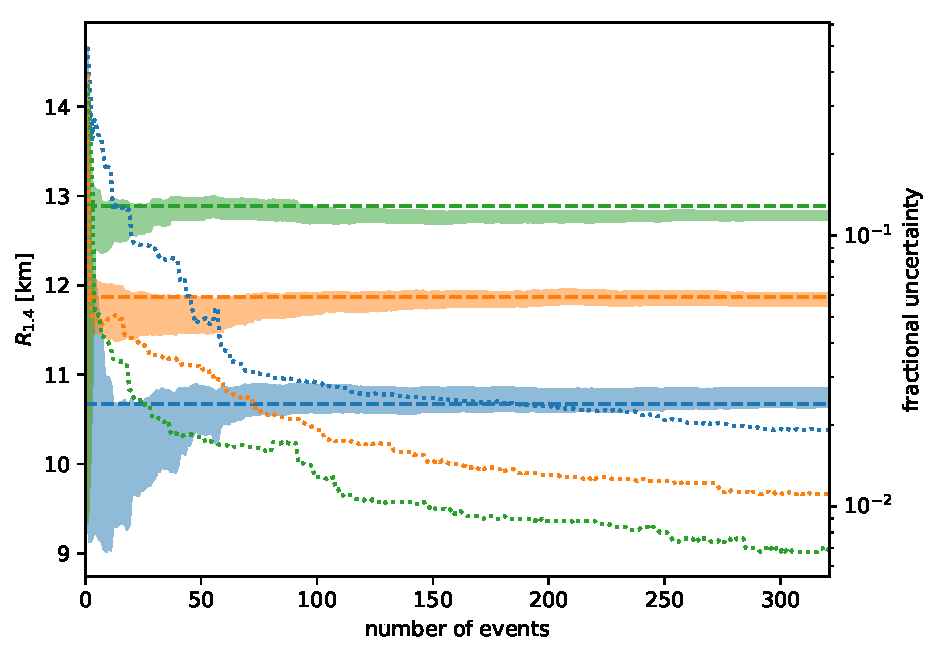
\includegraphics[width=\textwidth]{Figures/eos-meas/final_pop_hlv_combined_radius_3eos_gaussian_prior_seed0_bw0p3.pdf}
\caption{Combined $R_{1.4}$ measurements for our Gaussian mass distributed population in the LIGO-Virgo network. Results are shown for the soft (blue), medium (orange), and stiff (green) equations of state that we used. Signals are combined one at a time to show an updating constraint on the measurement as each signal is added. Shaded regions represent the 90\% credible interval for each measurement. The true values of $R_{1.4}$ for each of the equations of state are plotted as horizontal dashed lines in the appropriate color. Dotted lines show the fractional uncertainty in the measurement at each number of signals included, measured as the ratio of the 90\% credible interval to the true value of $R_{1.4}$ for a given equation of state.}
\label{fig:hlv_combined}
\end{figure}

% aLIGO default with SNR < 30
Constraints at intermediate numbers of signals will depend on the particular order in which the signals are combined, but we attempt to determine a general threshold for 10\% precision in two ways: 1. we perform the signal combination for 10 random permutations of the order; 2. we remove all signals with signal-to-noise $\rho>30$ and combine the remainder of the population to prevent any outsize influence from anomalously loud events. With both methods we find that a 10\% precision threshold is achieved after combining roughly 50 signals. This is consistent with other works that have found a better than 10\% constraint for similar numbers of signals seen by the LIGO-Virgo network~\cite{Lackey:2014fwa,Vivanco:2019qnt}. In Figure~\ref{fig:hlv_combined_snr_lt_30} we plot the result of combining the 277  signals in the population with $\rho < 30$. The final $R_{1.4}$ constraint for each of the equations of state is a factor of roughly 1.5 larger than was found for the entire population as a consequence of removing the loudest signals.

\begin{figure}[ht]
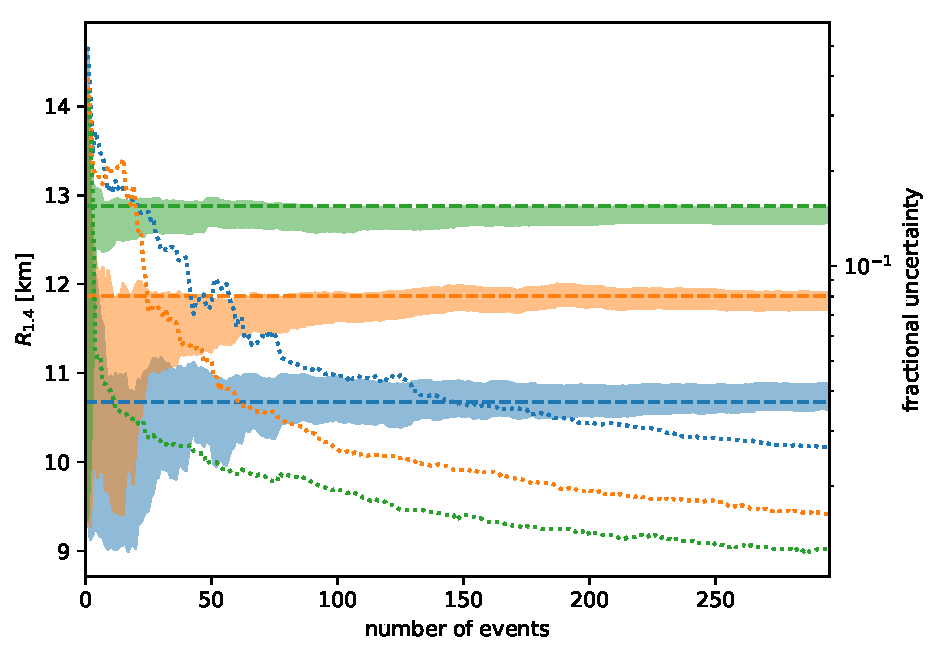
\includegraphics[width=\textwidth]{Figures/eos-meas/final_pop_hlv_combined_radius_3eos_gaussian_prior_seed0_bw0p3_snr_lt_30.pdf}
\caption{Same as Figure~\ref{fig:hlv_combined} except including only signals with signal-to-noise $\rho<30$. By removing louder signals we attempt to mitigate any potentially outsize effect on the radius constraint from signals that are unlikely to be seen by the LIGO-Virgo network. For the stiff, medium, and soft equations of state we find that a 10\% precision measurement on $R_{1.4}$ is reached after 5, 30, and 50 signals, respectively.}
\label{fig:hlv_combined_snr_lt_30}
\end{figure}

% aLIGO uniform (wrong) prior
In previous works it has been shown that imperfect knowledge of the mass distribution of neutron stars can introduce a bias into the equation of state measurement, owing to the mass dependence of the tidal deformability~\cite{Agathos:2015uaa,Wysocki:2020myz}. To investigate the implications of this effect in the context of precision equation of state measurements, we repeat our analysis on the Gaussian distributed mass population using a prior on the component masses that is uniform in the range $1-2$\msun. The combined $R_{1.4}$ constraint results from this analysis can be seen in Figure~\ref{fig:hlv_combined_uniform_prior}, where the signal ordering is the same as in Figure~\ref{fig:hlv_combined} for the sake of comparison. We find a small but significant bias toward smaller radii in our $R_{1.4}$ measurement for all three equations of state in our analysis, although the statistical uncertainties are not significantly changed. For EOS 1250 and EOS 895, we find the bias is enough to exclude the true value of $R_{1.4}$ at very high confidence after combining about 20 and 100 signals, respectively.

\begin{figure}[ht]
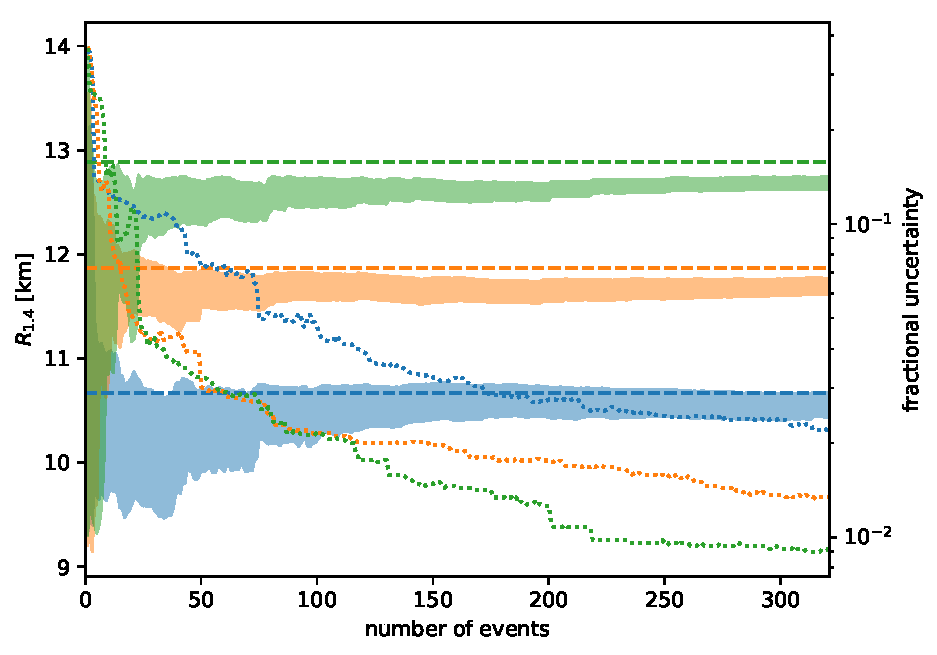
\includegraphics[width=\textwidth]{Figures/eos-meas/final_pop_hlv_combined_radius_3eos_uniform_prior_seed0_bw0p35.pdf}
\caption{Same as Figure~\ref{fig:hlv_combined} except we recover all signals with a uniform prior on the source-frame component masses from $1-2$\msun. This incorrect choice of mass prior introduces a bias in the equation of state measurement, leading to systematically lower estimates of $R_{1.4}$. We find that for EOS 1250 and EOS 895 the bias causes the true equation of state to be ruled out at high confidence after about 20 and 100 signals, respectively.}
\label{fig:hlv_combined_uniform_prior}
\end{figure}

% aLIGO uniform population
We investigate also the effect on a precision equation of state constraint from a neutron star mass distribution with greater representation of higher mass stars, since larger masses correspond to smaller $\Lambda$. To do this we perform our analysis on a population that is drawn uniformly in neutron star masses from $1-2$\msun. The combined $R_{1.4}$ constraint results are shown in Figure~\ref{fig:hlv_combined_uniform_pop}. We find for each equation of state we analyze the $R_{1.4}$ constraint is essentially unchanged from the Gaussian distributed population analysis, with final measurement precisions ranging from $1-2\%$.

\begin{figure}[ht]
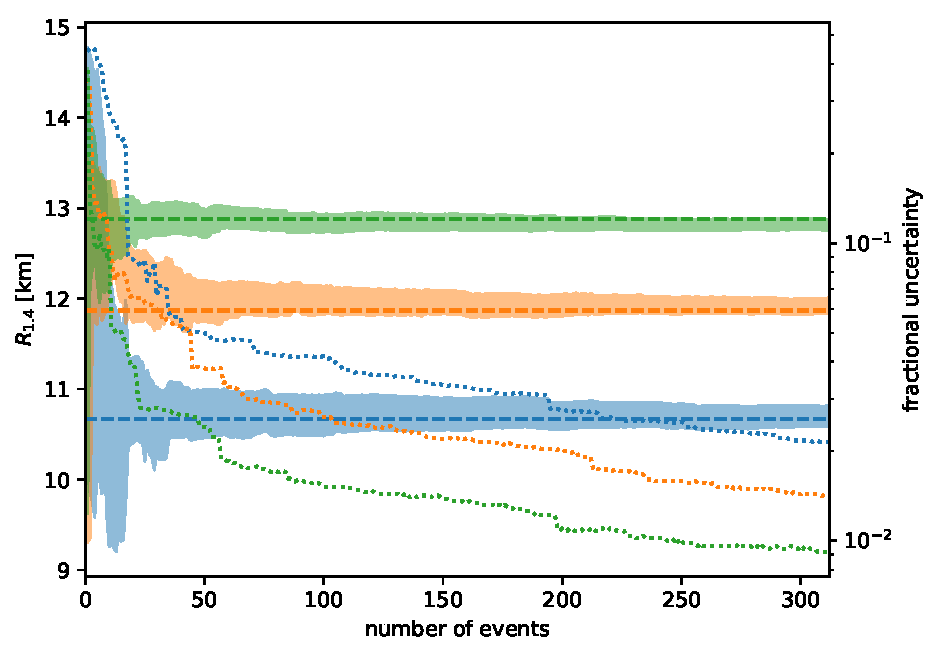
\includegraphics[width=\textwidth]{Figures/eos-meas/final_pop_hlv_combined_radius_3eos_uniform_prior_uniform_pop_seed3_bw0p3_312events.pdf}
\caption{
Combined $R_{1.4}$ measurements for our uniform mass population in the LIGO-Virgo network. Source-frame component masses are drawn from $1-2$\msun\ to represent a population with more high-mass neutron stars. All signals are recovered with a uniform mass prior from $1-2$\msun\ and signals are combined following the same procedure as the Gaussian mass population. We find the combined equation of state measurements from the uniform mass population are essentially unchanged from the Gaussian mass population, with precision on the measurement of $R_{1.4}$ ranging from $1-2\%$. 
}
\label{fig:hlv_combined_uniform_pop}
\end{figure}

% aLIGO probability of seeing events
While our LIGO-Virgo analysis includes hundreds of binary neutron star signals to produce a combined constraint, it is not at all certain that the merger rate and detector sensitivity will produce so many signals. To convert our signal-number forecast to a potential time horizon, we estimate the probability of seeing different numbers of events, assuming any population of mergers in the local universe will follow the universal analytic signal-to-noise distribution described in \cite{Chen:2014yla}. We calculate this probability as a function of the total number of events, and we convert that to number of years at the projected sensitivity for the upcoming fourth LIGO observing run (O4). We use the median binary neutron star merger rate estimate $\mathcal{R}=320~\mathrm{Gpc}^{-3}\mathrm{yr}^{-1}$ from \cite{Abbott:2020gyp}, the projected O4 search volume $VT=0.016~\mathrm{Gpc}^{3}\mathrm{yr}$ from \cite{Aasi:2013wya}, and we assume a detection threshold network signal-to-noise $\rho_{t}=9$. The calculated probabilities of seeing 10, 25, and 50 events with $\rho > 10$, consistent with the signals we include in this work, can be seen in Figure~\ref{fig:prob_of_events}. We note that O4 is expected to last approximately one year, though we calculate probabilities beyond that timeline to allow for any delays in the planned detector upgrades and to provide a lower limit for future observing runs that are expected to operate with improved sensitivity. We find that while 10 binary neutron star signals with $\rho>10$ will almost certainly be seen in just 3 years of observation at O4 sensitivity, it will take over 12 years at this sensitivity to have any significant probability of seeing 50 signals.

\begin{figure}[ht]
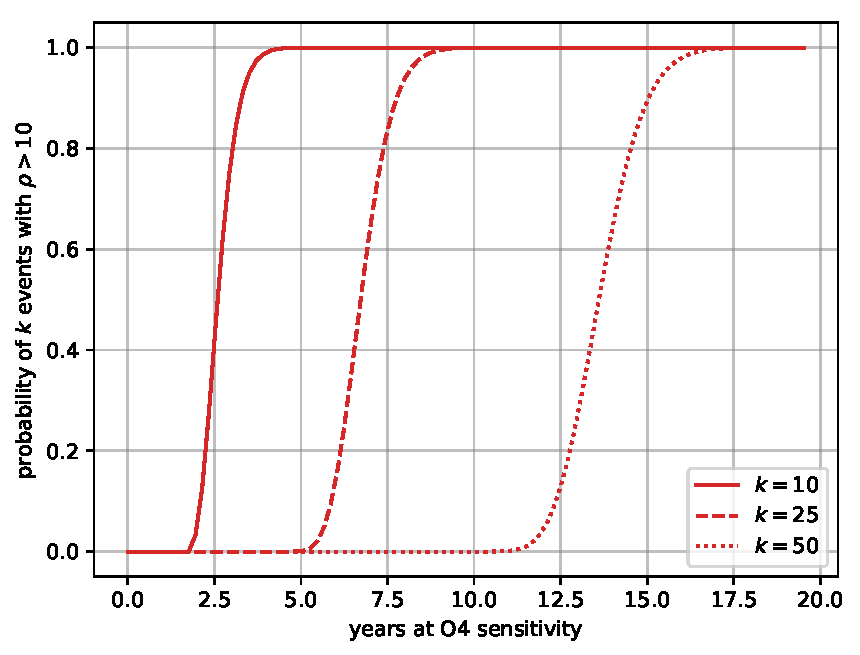
\includegraphics[width=\textwidth]{Figures/eos-meas/probability_over_time_snr10.pdf}
\caption{Probability of seeing 10, 25, and 50 events with signal-to-noise $\rho>10$ over time, assuming the population of merging binary neutron stars in the local universe follows the universal signal-to-noise distribution described in~\cite{Chen:2014yla}. The probabilities for 10, 25, and 50 events are shown as solid, dashed, and dotted lines, respectively. We use the median binary neutron star merger rate estimate from \cite{Abbott:2020gyp} and the projected sensitive volume for the upcoming fourth observing run (O4) of the Advanced LIGO network~\cite{Aasi:2013wya} to plot probabilities against number of years at O4 sensitivity. We assume a detection threshold network signal-to-noise ratio of 9.}
\label{fig:prob_of_events}
\end{figure}

Planned upgrades are expected to substantially increase detector sensitivity for the fifth observing run and beyond, though no official estimate of the search volume has yet been published. An improved network sensitivity would effectively shift the probability curves in Figure~\ref{fig:prob_of_events} leftward by the factor of improvement in search volume, though we note that even an order of magnitude improvement would likely result in at most 50 signals in several years of observation under the assumptions made here.

% CE default result
Finally, we explore the ability of Cosmic Explorer to precisely measure the equation of state. The extreme sensitivity of the Cosmic Explorer design means that it is expected to be sensitive to the complete population of merging binaries out to a redshift of $z=1$~\cite{CEHS}. This means that given current merger rate estimates, Cosmic Explorer will likely see hundreds of binary neutron star signals with $\rho>100$ in a single year of observation, and our simulated population of 335 signals is approximately representative of that set. The combined $R_{1.4}$ constraint for EOS 487 and EOS 895 are shown in Figure~\ref{fig:ce_combined}. We find that for both equations of state a 10\% precision threshold is achieved almost immediately, with the precision improving to 0.6\% and 0.15\% after combining all signals for EOS 487 and EOS 895, respectively. We also note that these constraint projections are likely slight overestimates, as there will be many more signals with $\rho<100$ seen in one year of observation that would still contain measurable tidal information. While the combined equation of state measurement will almost certainly be dominated by the louder signals we consider here, it is possible that quieter signals will contribute to improve the constraint somewhat.

\begin{figure}[ht]
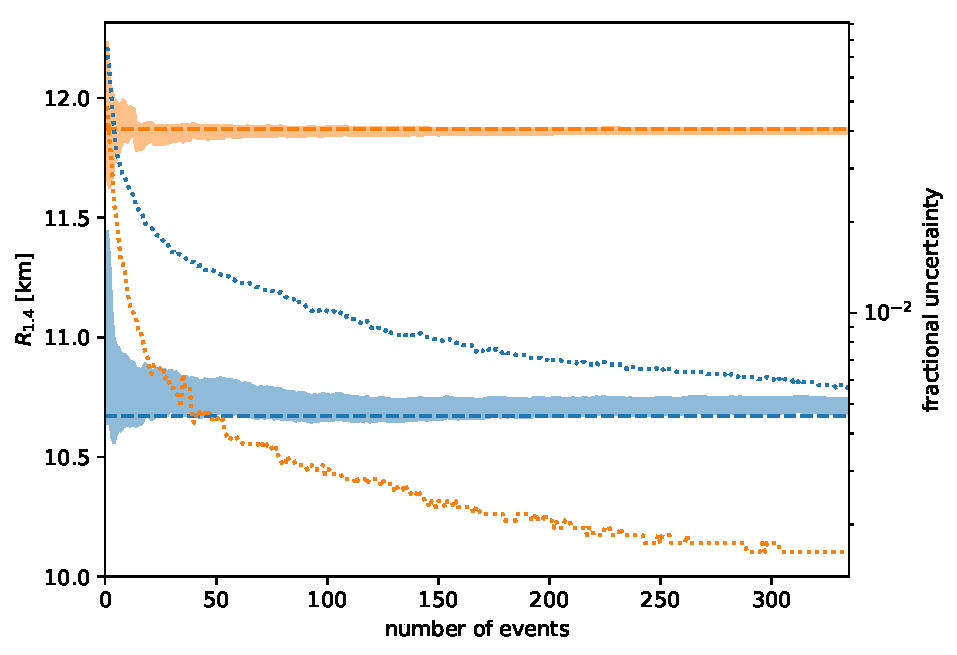
\includegraphics[width=\textwidth]{Figures/eos-meas/final_pop_ce_combined_radius_3eos_gaussian_prior_seed1_bw0p3.pdf}
\caption{
Combined $R_{1.4}$ measurements for our Gaussian mass distributed population in Cosmic Explorer, which is representative of the signals expected in one year of observation. Results are shown for the soft (blue) and medium (orange) equations of state in our analysis. As in Fig.~\ref{fig:hlv_combined} the horizontal dashed lines indicate the true value of $R_{1.4}$ for each equation of state, and the dotted lines show the calculated fractional uncertainty which is defined as the ratio of the 90\% credible interval to the true value of $R_{1.4}$. We find that for both equations of state, a 10\% precision threshold on the measurement of $R_{1.4}$ is achieved almost immediately, consistent with the third-generation detector result from~\cite{Pacilio:2021jmq}. The measurement precision improves to 0.6\% and 0.15\% for the soft and medium equations of state, respectively, after all signals are combined.
}
\label{fig:ce_combined}
\end{figure}

% CE uniform (wrong) prior result
We also check whether the Cosmic Explorer constraints are robust to an incorrect choice of mass prior by repeating the analysis using a uniform mass prior from $1-2$\msun. Systematic biases from an incorrect choice of prior are smaller for louder signals, so we expect that our population of Cosmic Explorer signals will suffer less from this effect. Figure~\ref{fig:ce_combined_uniform} shows the combined $R_{1.4}$ constraints from this analysis for the medium and soft equations of state we investigated, where again the ordering has been preserved from Figure~\ref{fig:ce_combined} to allow easy comparison. We find there is again a bias toward smaller radii for both EOS 487 and EOS 895, though it is much smaller in absolute terms than that seen in the LIGO-Virgo analysis. Still, the correspondingly smaller statistical uncertainties on our combined measurements make it so the true $R_{1.4}$ values lie right at the upper boundary of the 90\% credible interval for both equations of state, emphasizing the need for a good estimate of the neutron star mass distribution even for Cosmic Explorer. As was the case in our LIGO-Virgo analysis, we find the statistical uncertainties on the combined measurements are largely unchanged from the Gaussian mass prior analysis.

\begin{figure}[ht]
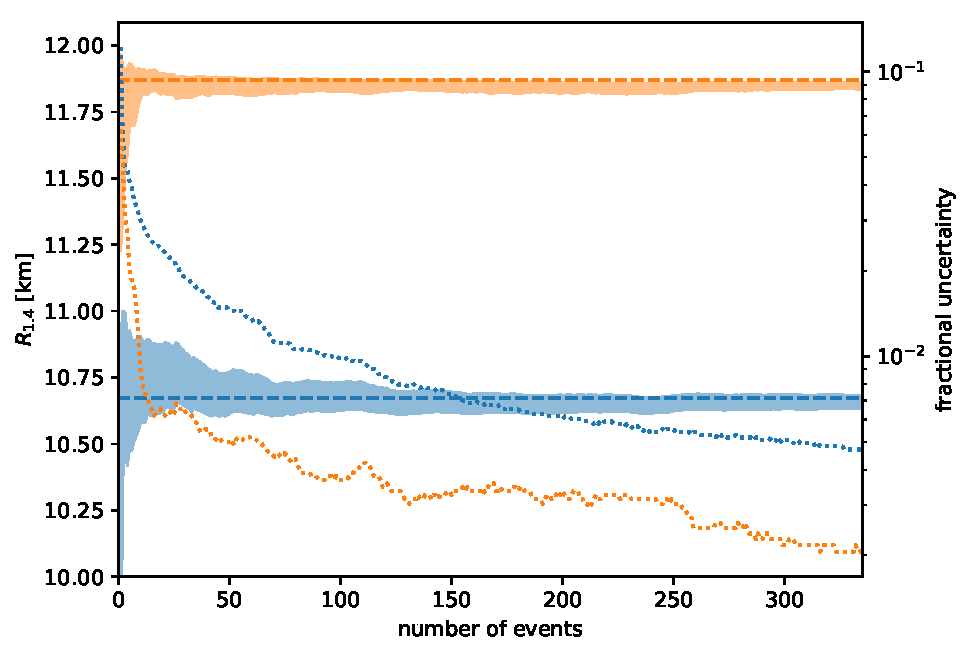
\includegraphics[width=\textwidth]{Figures/eos-meas/final_pop_ce_combined_radius_3eos_uniform_prior_seed1_bw0p3.pdf}
\caption{Same as Figure~\ref{fig:ce_combined} except we recover signals using a uniform mass prior from $1-2$\msun. The ordering of signals has been preserved from the Gaussian prior analysis for comparison, and it can be seen that the combined constraints for both equations of state is again biased toward smaller radii as a result of the incorrect mass prior. The bias is smaller than what was seen in our LIGO-Virgo analysis as a result of the much louder signals in the Cosmic Explorer population, however the true values for both equations of state are still found at the edge of their respective 90\% credible interval because of the correspondingly smaller statistical uncertainties on these measurements.}
\label{fig:ce_combined_uniform}
\end{figure}

\section{Conclusion}\label{sec:eos_meas_conclusion}
We  presented an updated forecast using more plausible equations of state for  binary neutron star mergers seen  by a LIGO-Virgo network, and new results for the proposed Cosmic Explorer detector. We use the most up-to-date estimates for the range of plausible equations of state and of the merger rate in the local universe. We find that Advanced LIGO will constrain $R_{1.4}$ to within 10\% at 90\% confidence with the first 50 signals, largely consistent with previous works, and we show that this projection is robust to a change in the mass population of neutron stars. We also extend the projection to find that across the full range of plausible equations of state, Advanced LIGO will be able to measure $R_{1.4}$ to better than about 2\% after 321 signals, although the probability of seeing this many signals before third generation detectors become operational is potentially  very low. On the other hand we find that the much greater sensitivity of Cosmic Explorer means it will be able to measure $R_{1.4}$ to better than 0.6\% at 90\% confidence across the full range of plausible equations of state with one year of observation. This precision from Cosmic Explorer will be sufficient to distinguish even similarly soft equations of state from one another at high confidence.

% mass prior effect
As discussed by Wysocki {\it et al.}, our analysis confirms that accurate knowledge of the mass distribution of neutron stars in the population of merging binaries is vital to making an unbiased measurement of the equation of state. We find that biases due to an incorrect mass prior can be present even in measurements from a population of loud signals in a third-generation detector like Cosmic Explorer, and as such we emphasize the added importance of efforts to mitigate these biases in the context of precision equation of state measurements.





\Chapter{Conclusions}
\label{ch:conclusions}
In the current era of gravitational-wave astrophysics we are moving beyond first direct detections and first multimessenger observations, to now making routine discoveries that deepen our understanding of the compact objects in our cosmic neighborhood. The LIGO-Virgo gravitational-wave detector network has detected 52 confirmed binary merger observations so far, and the detection rate has only accelerated as improved detector sensitivity extends our reach deeper into the universe. From the two observed binary neutron star mergers, our knowledge of the dynamics of these events and of neutron star physics has grown dramatically. They have provided confirmation of binary neutron star mergers as a source of short gamma-ray bursts, and also as important sites of heavy element production through $r$-process nucleosynthesis that can help explain observed chemical abundances. They have also shown that it is possible to measure the tidal information in a gravitational-wave signal to meaningfully update our constraints on the nuclear equation of state. As the LIGO-Virgo detectors approach their design sensitivity, and as third-generation detectors begin to come online, we expect to see many more binary neutron star mergers in the coming years. We anticipate that these new detections will provide even further insights into the physics of neutron stars.

In this thesis we have studied binary neutron star mergers, through a combination of observations and computational modeling. Specifically we explore the ability of a gravitational-wave analysis to extract physical parameters of the binary system, and of the neutron stars involved in the merger. We investigate the impact of multimessenger information on a gravitational-wave analysis, and we study the measurability of the nuclear equation of state, both now and in the future.

We have presented an analysis of the binary neutron star merger GW170817 informed by electromagnetic distance measurements of its identified host galaxy, and we demonstrated that using an independent distance measurement in a gravitational-wave analysis can break the distance-inclination degeneracy to allow for much tighter constraints on the inclination angle of the binary. We find our improved measurement of the inclination supports models for a structured relativistic jet and its afterglow emission being viewed off-axis.

We have presented measurements of the tidal deformabilities and radii of the neutron stars in GW170817. Our analysis imposed a physical constraint to require that both neutron stars obey the same equation of state, and we used a prior on the leading order tidal parameter constructed to contain all physical models of the equation of state without biasing the measurement toward any particular model. We note that the methodology we employed could be adapted for the analysis of future binary neutron star merger events with similar masses. We find our results are broadly consistent with several other studies~\cite{Abbott:2018exr,Radice:2018ozg,Coughlin:2018fis,Capano:2019eae} which employed various methods to measure the tidal deformabilities and radii in their own analyses of GW170817.

We have presented a likelihood model developed for \textit{PyCBC Inference} that uses the relative binning parameter estimation technique to reduce computational cost for potential multimessenger gravitational-wave sources. We extended the work of previous implementations to make our relative likelihood model a coherent network statistic so that it can additionally measure sky locations. We validated the relative model on populations of simulated binary neutron star and simulated neutron star--black hole merger signals, and we showed that it is possible to seed the relative analysis with the best-fit template parameters from a low-latency search pipeline. We found that the parameter estimation for all signals in our simulated populations completed in less than 20 minutes, with sky localization and intrinsic parameter estimates that are comparable to analyses done with a standard non-relative likelihood.

We have presented a comprehensive study of the future prospects for a precise equation of state measurement from Advanced LIGO and Cosmic Explorer. We explored the measurability of the equation of state across the full parameter space allowed by combined constraints from astrophysical observations and nuclear experiments. We showed that a precision threshold for measurements to distinguish between substantially similar theoretical models for the equation of state is equivalent to measuring the radius of a 1.4\msun\ neutron star to better than $2\%$, and we presented a framework for combining individual equation of state measurements across entire populations to produce a combined, high-precision measurement. We found it is unlikely that Advanced LIGO will achieve $2\%$ precision in the next observing runs given current estimates of the merger rate for binary neutron stars, however Cosmic Explorer will measure the equation of state to better than $1\%$ within one year of operation. Our framework can be directly applied to any future signals from binary neutron star mergers, and we anticipate that the resulting precise knowledge of the true equation of state will be invaluable for efforts to model these merger events and their associated kilonovae.

%\appendix
%\chapter{}
%\label{}
%\input{}
\clearpage
\bibliographystyle{unsrt}
\bibliography{inc-angle-ref,common-radius-ref,rel-bin-pe-ref,eos-meas-ref,add-references}
\addcontentsline{toc}{chapter}{\numberline {Bibliography}}

\renewenvironment{thebibliography}[1]%
  {\begin{list}{\labelenumi\hss}%
     {\usecounter{enumi}\setlength{\labelwidth}{3em}%
      \setlength{\leftmargin}{5em}}}%
  {\end{list}}
\renewcommand{\bibitem}[1]{\item\label{#1}\relax}%
\renewcommand{\theenumi}{\arabic{enumi}}%
%\fi
%\clearpage
%\newpage

\setboolean{@twoside}{false}
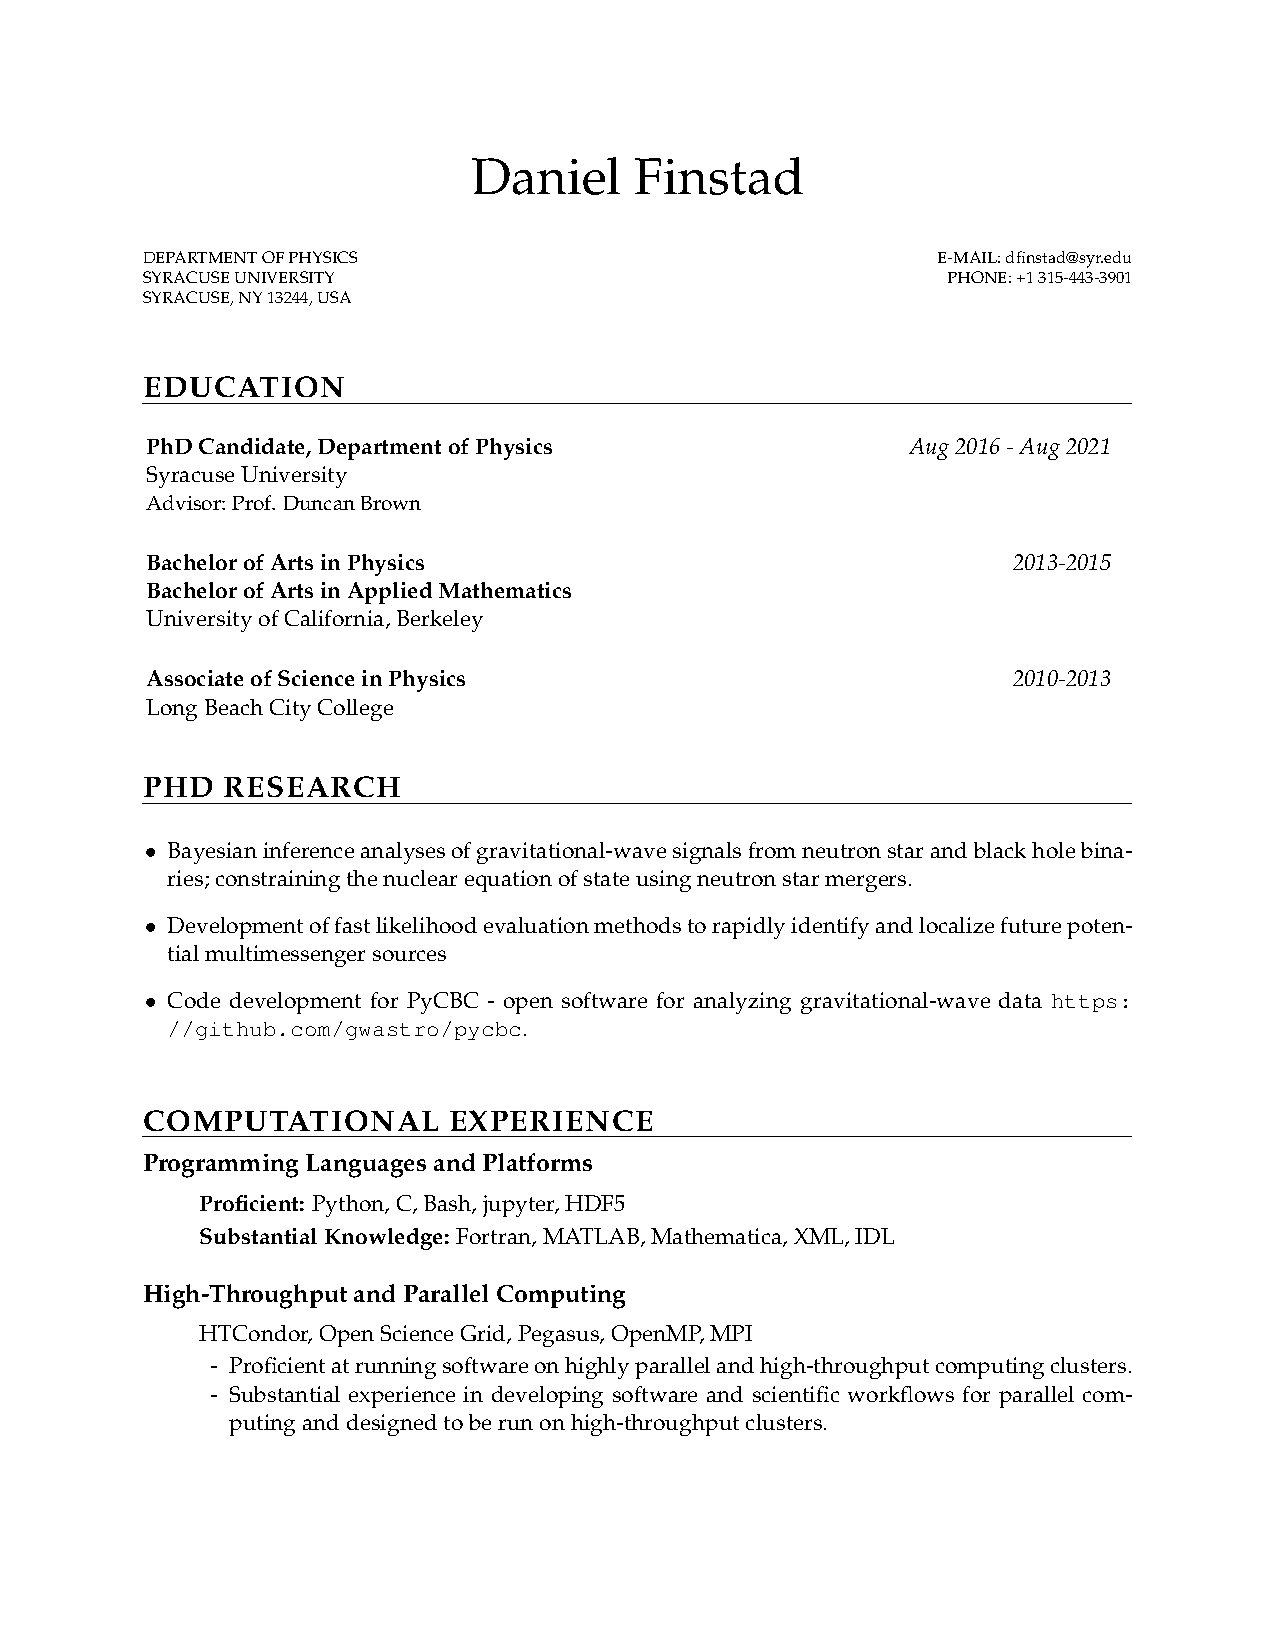
\includepdf[pages=-,pagecommand={}]{Daniel_Finstad_CV.pdf}

% The grad school requires the last page to be blank
\newpage
\thispagestyle{empty}
\end{document}
